\documentclass[a4paper,11pt,twoside]{report}
% THIS FILE SHOULD BE COMPILED BY pdfLaTeX

% ----------------------   PREAMBLE PART ------------------------------

% ------------------------ ENCODING & LANGUAGES ----------------------

\usepackage[utf8]{inputenc}
%\usepackage[MeX]{polski} % Not needed unless You have a name with polish symbols or sth
\usepackage[T1]{fontenc}
\usepackage[english, polish]{babel}
\usepackage{biblatex}
\usepackage{xcolor}
\usepackage{subcaption}
\addbibresource{references.bib}

\usepackage{amsmath, amsfonts, amsthm, latexsym} % MOSTLY MATHEMATICAL SYMBOLS

\usepackage[final]{pdfpages} % INPUTING TITLE PDF PAGE - GENERATE IT FIRST!
%\usepackage[backend=bibtex, style=verbose-trad2]{biblatex}


\usepackage{commath} % various commands which can make writing math expressions easier --- documentation available at: https://ctan.gust.org.pl/tex-archive/macros/latex/contrib/commath/commath.pdf

\usepackage[hidelinks]{hyperref} % for hyperlinks, for example, urls, references to equations, entries in a bibliography --- hidelinks option removes rectangles around hiperlinks


% ---------------- MARGINS, INDENTATION, LINESPREAD ------------------

\usepackage[inner=20mm, outer=20mm, bindingoffset=10mm, top=25mm, bottom=25mm]{geometry} % MARGINS


\linespread{1.5}
\allowdisplaybreaks         % ALLOWS BREAKING PAGE IN MATH MODE

\usepackage{indentfirst}    % IT MAKES THE FIRST PARAGRAPH INDENTED; NOT NEEDED
\setlength{\parindent}{5mm} % WIDTH OF AN INDENTATION


%---------------- RUNNING HEAD - CHAPTER NAMES, PAGE NUMBERS ETC. -------------------

\usepackage{fancyhdr}
\pagestyle{fancy}
\fancyhf{}
% PAGINATION: LEFT ALIGNMENT ON EVEN PAGES, RIGHT ALIGNMENT ON ODD PAGES 
\fancyfoot[LE,RO]{\thepage} 
% RIGHT HEADER: zawartość \rightmark do lewego, wewnętrznego (marginesu) 
\fancyhead[LO]{\sc \nouppercase{\rightmark}}
% lewa pagina: zawartość \leftmark do prawego, wewnętrznego (marginesu) 
\fancyhead[RE]{\sc \leftmark}

\renewcommand{\chaptermark}[1]{\markboth{\thechapter.\ #1}{}}

% HEAD RULE - IT'S A LINE WHICH SEPARATES HEADER AND FOOTER FROM CONTENT
\renewcommand{\headrulewidth}{0 pt} % 0 MEANS NO RULE, 0.5 MEANS FINE RULE, THE BIGGER VALUE THE THICKER RULE


\fancypagestyle{plain}{
  \fancyhf{}
  \fancyfoot[LE,RO]{\thepage}
  
  \renewcommand{\headrulewidth}{0pt}
  \renewcommand{\footrulewidth}{0.0pt}
}



% --------------------------- CHAPTER HEADERS ---------------------

\usepackage{titlesec}
\titleformat{\chapter}
  {\normalfont\Large \bfseries}
  {\thechapter.}{1ex}{\Large}

\titleformat{\section}
  {\normalfont\large\bfseries}
  {\thesection.}{1ex}{}
\titlespacing{\section}{0pt}{30pt}{20pt} 

    
\titleformat{\subsection}
  {\normalfont \bfseries}
  {\thesubsection.}{1ex}{}


% ----------------------- TABLE OF CONTENTS SETUP ---------------------------

\def\cleardoublepage{\clearpage\if@twoside
\ifodd\c@page\else\hbox{}\thispagestyle{empty}\newpage
\if@twocolumn\hbox{}\newpage\fi\fi\fi}


% THIS MAKES DOTS IN TOC FOR CHAPTERS
\usepackage{etoolbox}
\makeatletter
\patchcmd{\l@chapter}
  {\hfil}
  {\leaders\hbox{\normalfont$\m@th\mkern \@dotsep mu\hbox{.}\mkern \@dotsep mu$}\hfill}
  {}{}
\makeatother

\usepackage{titletoc}
\makeatletter
\titlecontents{chapter}% <section-type>
  [0pt]% <left>
  {}% <above-code>
  {\bfseries \thecontentslabel.\quad}% <numbered-entry-format>
  {\bfseries}% <numberless-entry-format>
  {\bfseries\leaders\hbox{\normalfont$\m@th\mkern \@dotsep mu\hbox{.}\mkern \@dotsep mu$}\hfill\contentspage}% <filler-page-format>

\titlecontents{section}
  [1em]
  {}
  {\thecontentslabel.\quad}
  {}
  {\leaders\hbox{\normalfont$\m@th\mkern \@dotsep mu\hbox{.}\mkern \@dotsep mu$}\hfill\contentspage}

\titlecontents{subsection}
  [2em]
  {}
  {\thecontentslabel.\quad}
  {}
  {\leaders\hbox{\normalfont$\m@th\mkern \@dotsep mu\hbox{.}\mkern \@dotsep mu$}\hfill\contentspage}
\makeatother



% ---------------------- TABLES AD FIGURES NUMBERING ----------------------

\renewcommand*{\thetable}{\arabic{chapter}.\arabic{table}}
\renewcommand*{\thefigure}{\arabic{chapter}.\arabic{figure}}


% ------------- DEFINING ENVIRONMENTS FOR THEOREMS, DEFINITIONS ETC. ---------------

\makeatletter
\newtheoremstyle{definition}
{3ex}%                           % Space above
{3ex}%                           % Space below
{\upshape}%                      % Body font
{}%                              % Indent amount
{\bfseries}%                     % Theorem head font
{.}%                             % Punctuation after theorem head
{.5em}%                          % Space after theorem head, ' ', or \newline
{\thmname{#1}\thmnumber{ #2}\thmnote{ (#3)}}
\makeatother

\theoremstyle{definition}
\newtheorem{theorem}{Theorem}[chapter]
\newtheorem{lemma}[theorem]{Lemma}
\newtheorem{example}[theorem]{Example}
\newtheorem{proposition}[theorem]{Proposition}
\newtheorem{corollary}[theorem]{Corollary}
\newtheorem{definition}[theorem]{Definition}
\newtheorem{remark}[theorem]{Remark}

% --------------------- END OF PREAMBLE PART (MOSTLY) --------------------------





% -------------------------- USER SETTINGS ---------------------------

\usepackage{float}
\usepackage{listings}
\usepackage{xcolor}
\usepackage{menukeys}
\usepackage{array}
\usepackage{graphicx}
\usepackage{caption}
\usepackage{subcaption}

\lstdefinelanguage{json}{
    basicstyle=\normalfont\ttfamily,
    numbers=left,
    numberstyle=\scriptsize,
    stepnumber=1,
    numbersep=8pt,
    showstringspaces=false,
    breaklines=true,
    frame=lines,
    backgroundcolor=\color[rgb]{0.95, 0.95, 0.95},
    stringstyle=\color[rgb]{0.25,0.5,0.35},
    keywordstyle=\color[rgb]{0.5,0.0,0.35},
    commentstyle=\color[rgb]{0.5,0.5,0.5},
    string=[s]{"}{"},
    comment=[l]{//},
    morecomment=[s]{/*}{*/},
    tabsize=2,
    keywords={},
}

\newcommand{\tytul}{Proceduralne generowanie świata i wyzwania związane z renderowaniem w przestrzeniach nieeuklidesowych}
\renewcommand{\title}{Procedural world generation and the challenges of rendering in non-Euclidean spaces}
\newcommand{\type}{Engineer} % Master OR Engineer
\newcommand{\supervisor}{Paweł Kotowski, Ph.D.} % TITLE AND NAME OF THE SUPERVISOR
\newcommand{\todo}[1]{\textbf{\textcolor{red}{TODO: #1}}}


\begin{document}
\sloppy
\selectlanguage{english}


\includepdf[pages=-]{title_page} % THIS INPUTS THE TITLE PAGE

\null\thispagestyle{empty}\newpage

% ------------------ PAGE WITH SIGNATURES --------------------------------

%\thispagestyle{empty}\newpage
%\null
%
%\vfill
%
%\begin{center}
%\begin{tabular}[t]{ccc}
%............................................. & \hspace*{100pt} & .............................................\\
%supervisor's signature & \hspace*{100pt} & author's signature
%\end{tabular}
%\end{center}
%


% ---------------------------- ABSTRACTS -----------------------------

{  \fontsize{12}{14} \selectfont
\begin{abstract}

    \begin{center}
        \title
    \end{center}
    Procedural generation, as a method used in creating video games, has experienced a significant increase in popularity in recent years.
    It has been employed extensively in acclaimed titles such as \textit{Minecraft} and \textit{No Man's Sky} to create virtually infinite worlds that the player is free to interact with.
    On the other hand, a recent game \textit{Hyperbolica} popularized a novel idea of making the virtual worlds even more interesting by setting them in non-Euclidean spaces.
    This work describes the implementation of a video game that incorporates both of the aforementioned concepts.

    In the game, we use and expand on the technique of transforming Euclidean space into hyperbolic or spherical space introduced by László Szirmay-Kalos and Milán Magdics in \cite{Szirmay-Kalos2022}.
    The approach allows for the use of established algorithms, developed with Euclidean geometry in mind, in other geometries.
    %This approach also simplifies the implementation of the game logic in different geometries as large parts of the implementation can be shared across the three geometries.
    Furthermore, core parts of the game logic can be shared between different geometries, which vastly simplifies the implementation.
    The approach also allows for changing the degree to which the scene is visually curved in hyperbolic geometry at runtime.

    The procedural terrain generation in the game is based on the marching cubes algorithm with Perlin noise used for generating the underlying scalar field.

    The game also includes several classic game features, such as terrain editing, character animations, day/night cycle, and many more.
    As a result, the game offers a unique experience of exploring and interacting with worlds inherently different from the one we live in. \\

    \noindent \textbf{Keywords:} Non-Euclidean Geometry, Hyperbolic Geometry, Spherical Geometry, Procedural Generation, Video Games, OpenGL, C\#
    \question{Should keywords start with capital letters?}
\end{abstract}
}

\null\thispagestyle{empty}\newpage


{\selectlanguage{polish} \fontsize{12}{14}\selectfont
\begin{abstract}

    \begin{center}
        \tytul
    \end{center}
    Proceduralne generowanie świata jest techniką zdobywającą rosnącą popularność przy tworzeniu gier komputerowych.
    Zostało ono wykorzystane z powodzeniem m. in. w takich produkcjach jak \textit{Minecraft} czy \textit{No Man's Sky}.
    Z drugiej strony za przyczyną gier takich jak \textit{Hyperbolica}, szersze zainteresowanie zyskała kwestia osadzania gier komputerowych w przestrzeniach nieeuklidesowych.
    Niniejsza praca opisuje implementację gry komputerowej, która łączy oba te podejścia.

    W grze zastosowano, z pewnymi modyfikacjami, metodę przekształcania przestrzeni euklidesowej w przestrzeń hiperboliczną lub sferyczną, zaproponowaną przez László Szirmay-Kalosa i Milána Magdicsa w \cite{Szirmay-Kalos2022}.
    Wspomniane podejście pozwala na wykorzystanie znanych algorytmów, zaprojektowanych z myślą o geometrii euklidesowej w innych geometriach.
    Dodatkowo, kluczowe części logiki gry mogą być dzięki temu dzielone pomiędzy różnymi geometriami, co znacznie upraszcza implementację.
    Zastosowana metoda pozwala również na zmianę stopnia zakrzywienia sceny w czasie rzeczywistym w przestrzeni hiperbolicznej.

    Proceduralne generowanie terenu w grze opiera się na algorytmie maszerujących sześcianów (ang. \textit{marching cubes algorithm}) z polem skalarnym określonym za pomocą szumu Perlina.

    Gra zawiera również wiele klasycznych funkcjonalności, takich jak edycja terenu, animacje postaci, cykl dnia i nocy oraz wiele innych.
    W rezultacie gra oferuje unikalne doświadczenie eksploracji i interakcji z światami fundamentalnie różnymi od tego, w którym żyjemy. \\

    \noindent \textbf{Słowa kluczowe:} geometria nieeuklidesowa, geometria hiperboliczna, geometria sferyczna, proceduralne generowanie terenu, gry komputerowe, OpenGL, C\#
\end{abstract}
}


%% --------------------------- DECLARATIONS ------------------------------------
%
%%
%%	IT IS NECESSARY OT ATTACH FILLED-OUT AUTORSHIP DEECLRATION. SCAN (IN PDF FORMAT) NEEDS TO BE PLACED IN scans FOLDER AND IT SHOULD BE CALLED, FOR EXAMPLE, DECLARATION_OF_AUTORSHIP.PDF. IF THE FILENAME OR FILEPATH IS DIFFERENT, THE FILEPATH IN THE NEXT COMMAND HAS TO BE ADJUSTED ACCORDINGLY.
%%
%%	command attacging the declarations of autorship
%%
%\includepdf[pages=-]{scans/declaration-of-autorship}
%\null\thispagestyle{empty}\newpage
%
%% optional declaration
%%
%%	command attaching the declaataration on granting a license
%%
%\includepdf[pages=-]{scans/declaration-on-granting-a-license}
%%
%%	.tex corresponding to the above PDF files are present in the 3. declarations folder 
%
\null\thispagestyle{empty}\newpage
% ------------------- TABLE OF CONTENTS ---------------------
% \selectlanguage{english} - for English
\pagenumbering{gobble}
\tableofcontents
\thispagestyle{empty}
\newpage % IF YOU HAVE EVEN QUANTITY OD PAGES OF TOC, THEN REMOVE IT OR ADD \null\newpage FOR DOUBLE BLANK PAGE BEFORE INTRODUCTION


% -------------------- THE BODY OF THE THESIS --------------------------------

\null\thispagestyle{empty}\newpage
\pagestyle{fancy}
\pagenumbering{arabic}
\setcounter{page}{11}

\chapter{Introduction}\label{ch:introduction}
\markboth{}{Introduction}
\addcontentsline{toc}{chapter}{Introduction}

What is the thesis about? What is the content of it? What is the Author's contribution to it?
\par
WARNING!  In a diploma thesis which is a team project: Description of the work division in the team, including the scope of each co-author’s contribution to the practical part (Team Programming Project) and the descriptive part of the diploma thesis.
\par

Lorem ipsum dolor sit amet, consetetur sadipscing elitr, sed diam nonumyeirmod tempor invidunt ut labore et dolore magna aliquyam erat, sed diamvoluptua. At vero eos et accusam et justo duo dolores et ea rebum. Stet clita kasd gubergren, no sea takimata sanctus est Lorem ipsum dolor sit amet. Lorem ipsum dolor sit amet, consetetur sadipscing elitr, sed diam nonumyeirmod tempor invidunt ut labore et dolore magna aliquyam erat, sed diamvoluptua. At vero eos et accusam et justo duo dolores et ea rebum. Stet clita kasd gubergren, no sea takimata sanctus est Lorem ipsum dolor sit amet.
\todo{What should be included in "Specyfikacja Funkcjonalna"? Just the user stories or maybe the whole deliverable 1?}
\chapter{Theoretical foundations}
\section{Non-Euclidean geometry} \label{sec:non_euclidean_geometry}

The \textit{Euclidean} geometry is based on a set of five postulates originally given by Euclid.
The postulates read as follows \cite{Weisstein-Postulates}:
\begin{enumerate}
    \item A straight line segment can be drawn joining any two points.
    \item Any straight line segment can be extended indefinitely in a straight line.
    \item Given any straight line segment, a circle can be drawn having the segment as the radius and one endpoint as the center.
    \item All right angles are congruent.
    \item Given any straight line and a point not on it, there exists one and only one straight line that passes through that point and never intersects the first line, no matter how far they are extended. \cite{Weisstein-Parallel}
\end{enumerate}
The fifth postulate, also called the \textit{parallel postulate}, has been for hundreds of years a subject of debate if it can be proven from the former four postulates.
It was discovered, however, that the negation of the parallel postulate doesn't lead to a contradiction \cite{Parallel-Postulate}.
The postulate can be negated in one of two ways.
\begin{itemize}
    \item Given any straight line and a point not on it, there exist \textbf{at least two straight lines} that pass through that point and never intersect the first line, no matter how far they are extended.
    \item Given any straight line and a point not on it, there exists \textbf{no straight line} that passes through that point and never intersects the first line; in other words, there are no parallel lines, since any two lines must intersect.
\end{itemize}

When the parallel postulate is replaced with the first statement, we obtain a new geometry, called the \textit{hyperbolic geometry}.
Similarly, replacing it with the second statement yields the \textit{spherical geometry}.
These geometries are collectively referred to as \textit{non-Euclidean geometries}.

\subsection{Analytic description}
To describe the non-Euclidean geometries analytically, we will follow the approach given by \cite{Szirmay-Kalos2022}.
This approach allows us to view the points of a 3-dimensional non-Euclidean space as a subset of the 4-dimensional \textit{embedding space}.
Since imagining the fourth dimension is not something particularly easy, we will be decreasing the dimensionality whenever we give examples.

The elliptic space can be modeled as a unit 3-sphere, \textit{embedded} in a 4-dimensional Euclidean space.
By saying that a space is embedded in another, we mean that the embedded space inherits the distance from the embedding space.
In this case, the spherical distance, given by $ds^2 = dx^2 + dy^2 + dz^2 + dw^2$ is derived from the Euclidean distance.
This is similar to how we may model the 2-dimensional elliptic space as a sphere, where lines are identified with great circles.
The inner product of two vectors $u$ and $v$ in the Euclidean space is given by
$$ \langle u, v \rangle_E  = u_xv_x + u_yv_y + u_zv_z + u_wv_w.$$
Thus, we can define that a point $p$ belongs to the elliptic geometry if
$$ \langle p, p \rangle_E = 1.$$

The model that we use for the hyperbolic geometry is the so-called \textit{hyperboloid model}.
In this model, points $p$ of the hyperbolic space satisfy the equation
$$p_x^2 + p_y^2 + p_z^2 - p_w^2 = -1,$$
with $p_w > 0$.
The set of these points creates the upper sheet of a hyperboloid, which could be visualized as shown in \autoref{fig:hyperboloid} if the embedding space was Euclidean.
\begin{figure}[h]
    \centering
    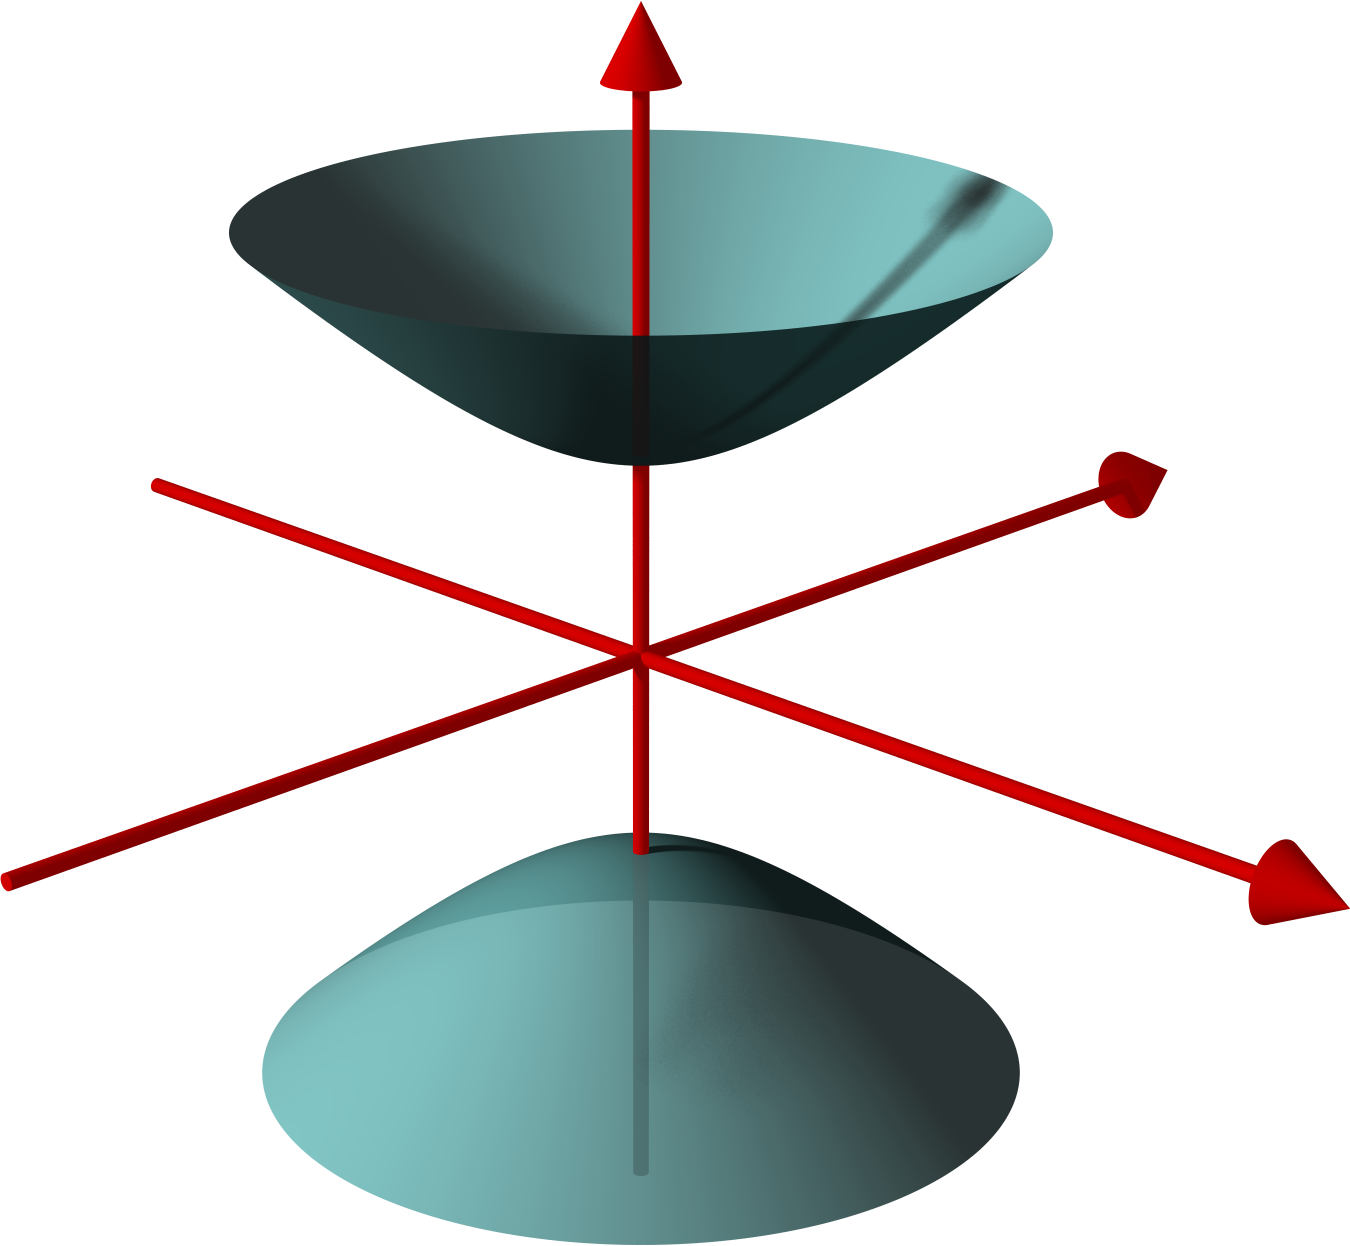
\includegraphics[width=0.4\textwidth]{chapters/theoretical_foundations/sections/non-eudlidean-spaces/resources/hyperboloid.png}
    \caption{2-dimensional hyperboloid embedded in Euclidean space}
    \label{fig:hyperboloid}
\end{figure}
However, the hyperbolic space is not embedded in the Euclidean space, but in the \textit{Minkowski space} instead.
In the Minkowski space, the inner product of vectors $u$, $v$ is given by the Lorentzian inner product:
$$\langle u, v \rangle_L = u_xv_x + u_yv_y + u_zv_z - u_wv_w.$$
Thus, the points $p$ belonging to the hyperbolic geometry satisfy the equation
$$\langle p, p \rangle_L = -1.$$
It could be interpreted that they are located on a sphere with a radius of imaginary length $\sqrt{-1}$ (and hence are equidistant from the origin).

To build a unified framework for discussing both types of geometries, we introduce the notion of \textit{sign of curvature}, $\mathcal{L}$, that attains the value $+1$ for spherical, and $-1$ for hyperbolic space.
We also define the generalized inner product
\begin{equation} \label{eq:gen-inner-prod}
    \langle u, v \rangle = u_xv_x + u_yv_y + u_zv_z + \mathcal{L}u_wv_w.
\end{equation}


\subsection{Transformations}
We will now define transformations that can be used in non-Euclidean geometries.

\subsubsection{Reflection}
A vector $v_R$ obtained from reflecting vector $v$ on vector $m$, see \autoref{fig:reflection}, can be defined as
\begin{figure}[h]
    \centering
    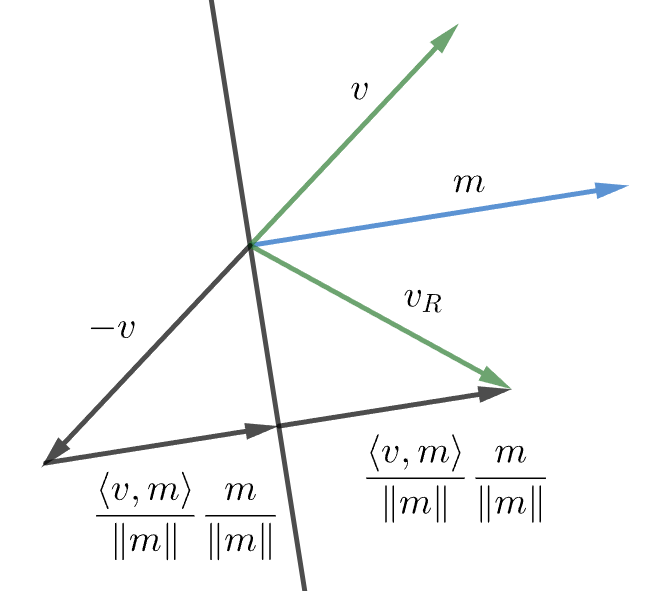
\includegraphics[width=0.4\textwidth]{chapters/theoretical_foundations/sections/non-eudlidean-spaces/resources/reflection.png}
    \caption{Reflection of $v$ on vector $m$}
    \label{fig:reflection}
\end{figure}
$$v_R = 2 \frac{\langle v, m \rangle}{\lVert m \rVert}\frac{m}{\lVert m \rVert} - v = 2\frac{\langle v, m\rangle}{\langle m,m\rangle}m - v.$$
It can be verified that this definition satisfies the intuitive conditions of a reflection:
\begin{itemize}
    \item The reflected vector $v_R$ lies in the plane spanned by $v$ and $m$,
    \item The transformation is an isometry, i.e. $\lVert u - v \rVert = \lVert u_R - v_R \rVert$.
\end{itemize}
We should also note that given a point $p$ in the geometry, i.e. satisfying $\langle p, p \rangle = \mathcal{L}$, its reflection, $p'$, is also in the geometry.

\subsubsection{Translation}
Just like in Euclidean space, we can define translation in terms of an even number of reflections.
More specifically, the translation will be defined by specifying two points: \textit{geometry origin}, $g = (0, 0, 0, 1)$ and \textit{translation target}, $q$, which is the point that the geometry origin is translated to.
Now we can define that the translation is the composition of two reflections: one on the vector $m_1 = g$ and the second one on the vector $m_2 = g + q$, which is halfway between $g$ and $q$.
Applying the first reflection to an arbitrary point $p$ gives a point
$$p' = 2 \frac{\langle p, g \rangle}{\langle g, g \rangle}g - p = 2p_w g - p,$$
and the second reflection applied to $p'$ yields a point
\begin{equation} \label{eq:translation}
    p'' = 2 \frac{\langle p', g + q \rangle}{\langle g + q, g + q \rangle}(g + q) - p'
    = 2 p_w q + p - \frac{p_w + \mathcal{L}\langle p, q \rangle}{1 + q_w}(g + q).
\end{equation}
The effect of applying translation to an arbitrary point $a$ is shown in \autoref{fig:translation}.\\
\begin{figure}[h]
    \centering
    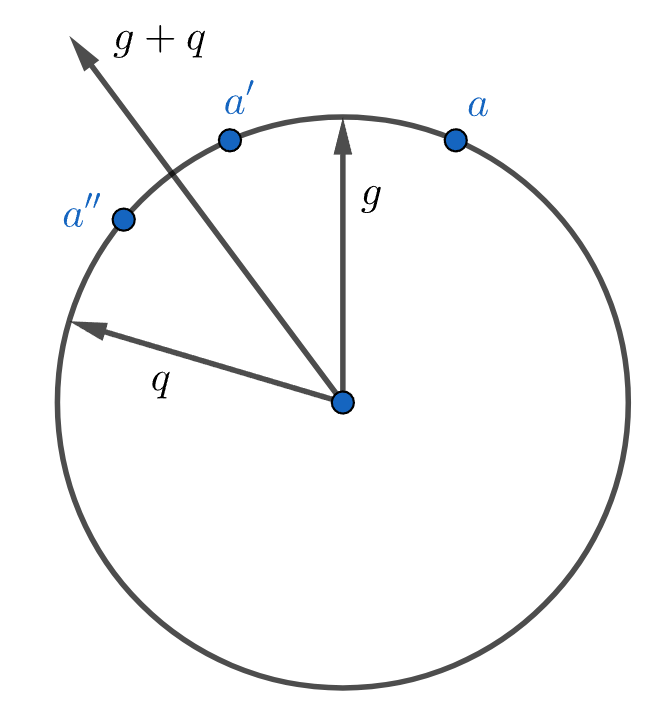
\includegraphics[width=0.4\textwidth]{chapters/theoretical_foundations/sections/non-eudlidean-spaces/resources/translation.png}
    \caption{Translation of a point $a$}
    \label{fig:translation}
\end{figure}
It can be verified that the geometry origin $g$ is indeed translated to point $g'' = q$.
We can evaluate the formula for the basis vectors $i = (1, 0, 0, 0)$, $j = (0, 1, 0, 0)$, $k = (0, 0, 1, 0)$, and $l = (0, 0, 0, 1)$ obtaining the translation matrix
\begin{equation} \label{eq:translation-matrix}
    T(q) = \begin{bmatrix}
        1 - \mathcal{L}\frac{q_x^2}{1 + q_w} & -\mathcal{L}\frac{q_x q_y}{1 + q_w}  & -\mathcal{L}\frac{q_x q_z}{1 + q_w}  & -\mathcal{L} q_x \\
        -\mathcal{L}\frac{q_y q_x}{1 + q_w}  & 1 - \mathcal{L}\frac{q_y^2}{1 + q_w} & -\mathcal{L}\frac{q_y q_z}{1 + q_w}  & -\mathcal{L} q_y \\
        -\mathcal{L}\frac{q_z q_x}{1 + q_w}  & -\mathcal{L}\frac{q_z q_y}{1 + q_w}  & 1 - \mathcal{L}\frac{q_z^2}{1 + q_w} & -\mathcal{L} q_z \\
        q_x                                  & q_y                                  & q_z                                  & q_w
    \end{bmatrix}
\end{equation}
It can be seen that the translation is an isometry since the row vectors of the matrix are orthonormal.

\subsubsection{Rotation}
It can be shown that a rotation about an axis through the origin is the same as the Euclidean rotation about the same axis \cite{Philips-Mark-Gunn1992}.

\subsubsection{Camera transformation}
% The camera transformation is defined in terms of the \textit{camera position} $e$, \textit{gaze direction} $g$, and the \textit{view-up vector} $t$.
% The camera position is a location that the camera "sees from", the gaze direction is a vector in the direction the camera is looking, and the view-up vector is a vector that points "to the sky".
% Using these vectors we can define the \textit{view space}, i.e. the camera's local coordinate system with the camera at the geometry origin and basis vectors $i'$, $j'$, and $k'$ defined as follows:
% \begin{equation*}
%     \begin{split}
%         k' = -\frac{g}{\lVert g \rVert}                    \\
%         i' = \frac{t \times k'}{\lVert t \times k' \rVert} \\
%         j' = k' \times i'
%     \end{split}
% \end{equation*}

The camera transformation allows us to describe the scene from the viewer's perspective.
The transformation is defined in terms of the \textit{eye position} $e$, and three orthonormal vectors in the tangent space of the eye:
\begin{enumerate}
    \item the right direction $i'$,
    \item the up direction $j'$, and
    \item the negative view direction $k'$.
\end{enumerate}
An example in \autoref{fig:tangent-space} shows the tangent space of the eye, with the $e$ vector marked green, $-k'$ marked blue, and $i'$ marked orange.\\
\begin{figure}[h]
    \centering
    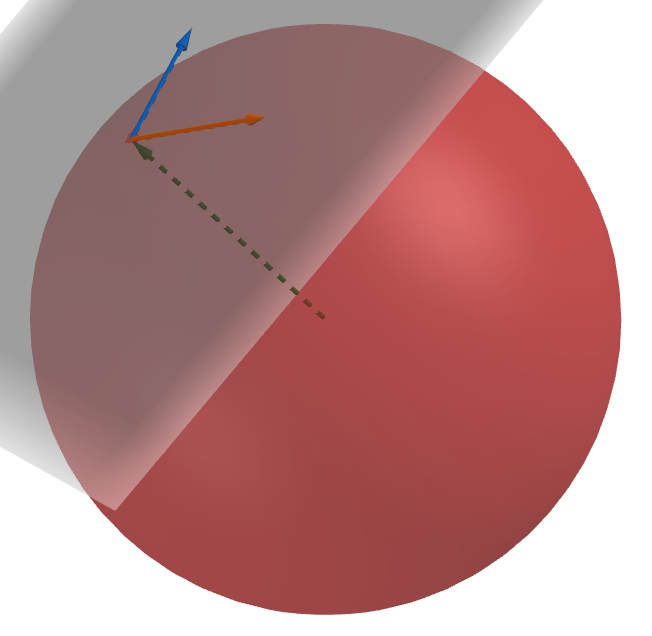
\includegraphics[width=0.4\textwidth]{chapters/theoretical_foundations/sections/non-eudlidean-spaces/resources/tangent-space.png}
    \caption{Tangent space of the camera}
    \label{fig:tangent-space}
\end{figure}
The transformation can be described by the matrix
\begin{equation} \label{eq:view-matrix}
    V =
    \begin{bmatrix}
        i'_x            & j'_x            & k'_x            & \mathcal{L}e_x \\
        i'_y            & j'_y            & k'_y            & \mathcal{L}e_y \\
        i'_z            & j'_z            & k'_z            & \mathcal{L}e_z \\
        \mathcal{L}i'_w & \mathcal{L}j'_w & \mathcal{L}l'_w & e_w
    \end{bmatrix}
\end{equation}
As the result of the transformation, the eye position is mapped to the geometry origin $g$.
Furthermore, the vectors $i'$, $j'$, and $k'$ are mapped to $i$, $j$, and $k$, respectively.

\subsubsection{Perspective transformation}
The perspective transformation is described using a projection matrix $P$.
The projection matrix we use in spherical geometry is identical to the one used in the \textit{Unity} implementation of \cite{Szirmay-Kalos2022} (see \url{https://github.com/mmagdics/noneuclideanunity}).
It is parameterized by the \textit{near plane distance} $n$, \textit{far plane distance} $f$, \textit{aspect ratio} ASP, and \textit{field of view} FOV:
\begin{equation*}
    P =
    \begin{bmatrix}
        s_x & 0   & 0  & 0  \\
        0   & s_y & 0  & 0  \\
        0   & 0   & 0  & -1 \\
        0   & 0   & -n & 0
    \end{bmatrix},
\end{equation*}
where $s_x = 2n / (r - l)$, $s_y = 2n / (t - b)$, and $r$, $l$, $t$, $b$ are defined in terms of $u = f \tan(\mathrm{FOV})$:
\begin{equation*}
    r = u \cdot \mathrm{ASP}, \,
    l = -u \cdot \mathrm{ASP}, \,
    t = u, \,
    b =  -u.
\end{equation*}
For hyperbolic and Euclidean geometries, the standard projection matrix is used.

\subsubsection*{Porting objects}
The positions of objects in the scene are specified in a 3-dimensional Euclidean space.
They are then "transported" or \textit{ported} to a non-Euclidean space of choice.
One possible mapping that could be used for this purpose is called the exponential map.
For a given point $p$ in the 3-dimensional Euclidean space with coordinates $(x, y, z)$ the mapping to elliptic geometry is given by
\begin{equation} \label{eq:elliptic-porting}
    \mathcal{P}_E(p) = (p / d \sin(d), \cos(d)),
\end{equation}
and for hyperbolic space, it is given by
\begin{equation*}
    \mathcal{P}_H(p) = (p / d \sinh(d), \cosh(d)),
\end{equation*}
where $d = \lVert p \rVert$.
The effect of porting a 1-dimensional point $p$ onto a 1-dimensional elliptic space can be seen in \autoref{fig:exp-map}.
\begin{figure}[h]
    \centering
    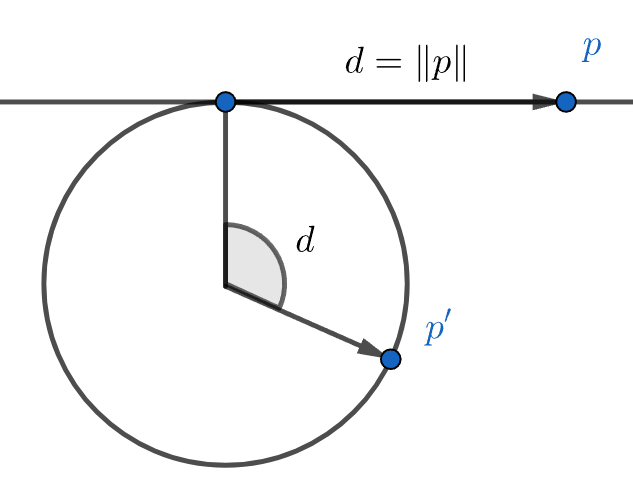
\includegraphics[width=0.4\textwidth]{chapters/theoretical_foundations/sections/non-eudlidean-spaces/resources/exp-map.png}
    \caption{Exponential map}
    \label{fig:exp-map}
\end{figure}

\subsubsection*{Porting vectors}
A vector $v$ starting at a point $p$ can be ported to non-Euclidean space by translating it to a point $\mathcal{P}(p)$.
Hence the ported vector $v'$ is given by
\begin{equation} \label{eq:porting-vector}
    v' = (v, 0) T(\mathcal{P}(p)),
\end{equation}
where $T$ is the translation matrix \ref{eq:translation-matrix}.
\subsection{Practical considerations} % based on scripts/distortions_calc.py
There are two ways we could implement placing objects in the scene:
\begin{enumerate}
    \item Port the object to non-Euclidean geometry and then use the translation given by \autoref{eq:translation},
    \item Translate the object using ordinary Euclidean translation and then port it to non-Euclidean geometry.
\end{enumerate}
The first option is undesirable, as it may significantly change the relative positions of objects in the scene.
To see why, let's consider two copies of a 2-dimensional rectangle that we will first port to the spherical geometry, and then translate using the non-Euclidean translation.
The rectangle with vertices $a = (-0.5, -0.7)$, $b = (0.5, -0.7)$, $c = (0.5, 0.5)$, $d = (-0.5, 0.5)$ is ported to spherical geometry using \autoref{eq:elliptic-porting}.
As a result, we obtain points on a unit sphere:
\begin{equation*}
    \begin{split}
         & \mathcal{P}(a) = (-0.441, -0.617, 0.652) \\
         & \mathcal{P}(b) = (0.441, -0.617, 0.652)  \\
         & \mathcal{P}(c) = (0.459, 0.459, 0.760)   \\
         & \mathcal{P}(d) = (-0.459, 0.459, 0.760)
    \end{split}
\end{equation*}
If we were to translate the first copy of the rectangle to point $t_1 = (0.5, 0.5)$ and the second copy to $t _2 = (1.5, 1.7)$ in Euclidean geometry, the two copies should meet at the point $(1, 1)$.

When we perform the translation to point $t_1$ (the corresponding translation target is obtained by porting $t_1$ using \autoref{eq:elliptic-porting}, i.e. the translation target is $q_1 = \mathcal{P}(t_1)$), we get the following vertices:
\begin{equation*}
    \begin{split}
         & T_{q_1}\mathcal{P}(a) =  (-0.014, -0.190, 0.982) \\
         & T_{q_1}\mathcal{P}(b) = (0.761, -0.296, 0.577)   \\
         & T_{q_1}\mathcal{P}(c) = (0.698, 0.698, 0.156)    \\
         & T_{q_1}\mathcal{P}(d) = (-0.110, 0.809, 0.578)
    \end{split}
\end{equation*}
The translation to $t_2$ (with $q_2 = \mathcal{P}(t_2)$) gives
\begin{equation*}
    \begin{split}
         & T_{q_2}\mathcal{P}(a) = (0.709, 0.686, 0.160)   \\
         & T_{q_2}\mathcal{P}(b) = (0.957, -0.031, -0.287) \\
         & T_{q_2}\mathcal{P}(c) = (0.141, 0.099, -0.985)  \\
         & T_{q_2}\mathcal{P}(d) = (-0.117, 0.847, -0.519)
    \end{split}
\end{equation*}
Even though we would expect the third vertex of the first copy of the rectangle to be identical to the first vertex of the second copy, there is a difference between the two.
This effect can be seen in \autoref{fig:spherical-rectangles}.
\begin{figure}[h]
    \centering
    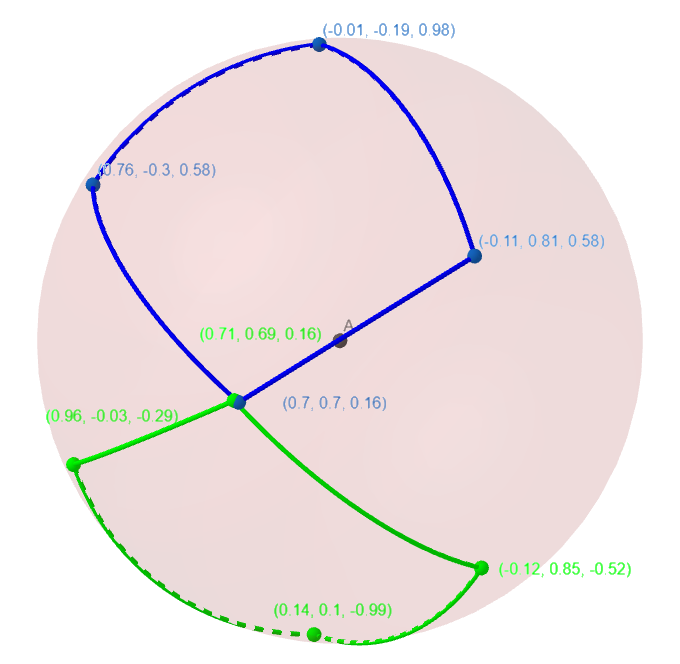
\includegraphics[width=0.6\textwidth]{chapters/theoretical_foundations/sections/non-eudlidean-spaces/resources/spherical-rectangles.png}
    \caption{Rectangles ported onto a sphere and then translated}
    \label{fig:spherical-rectangles}
\end{figure}
The effect is even more visible in the implementation. \autoref{fig:misaligned-wheel} shows how the wheels of the car get misaligned from their wheel arches.
\begin{figure}[h]
    \centering
    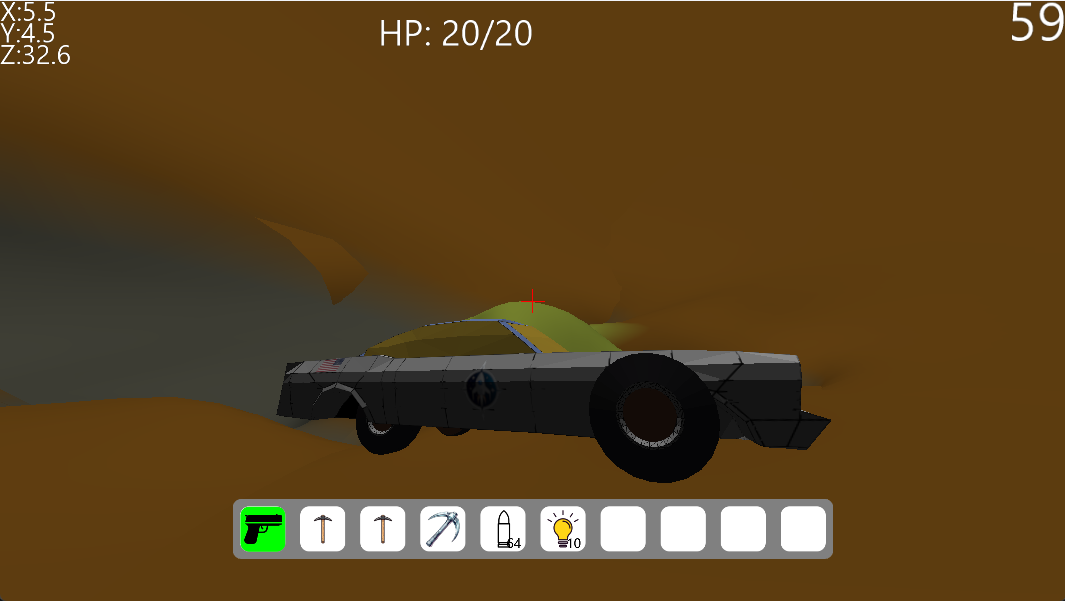
\includegraphics[width=0.6\textwidth]{chapters/theoretical_foundations/sections/non-eudlidean-spaces/resources/misaligned-wheel.png}
    \caption{Non-Euclidean translation causing a misalignment of objects}
    \label{fig:misaligned-wheel}
\end{figure}

The second option isn't unfortunately free of distortions as well.
For example, consider two identical squares of side length $0.5$.
The first one with the bottom-left corner at the point $(0,0)$ and the second one with the corresponding corner at $(0.5, 0.5)$.
After porting to spherical geometry using the \autoref{eq:elliptic-porting}, we get squares with side lengths (listed counter-clockwise starting at the bottom edge):
\begin{equation*}
    0.500, \,
    0.479, \,
    0.479, \,
    0.500
\end{equation*}
for the first square and with side lengths
\begin{equation*}
    0.480, \,
    0.425, \,
    0.425, \,
    0.480
\end{equation*}
for the second square.
The side lengths of the square have been calculated as the lengths of geodesics\footnote{This is the "great-circle distance" equal to $2 \arcsin{(c / 2)}$, where $c$ is the chord length.} between the square's vertices.
As we can see, the side lengths of the ported square are no longer equal to each other, and the distortion increases as the square is farther away from the origin.
This effect can be seen in \autoref{fig:bending-car}.
\begin{figure}[h]
    \centering
    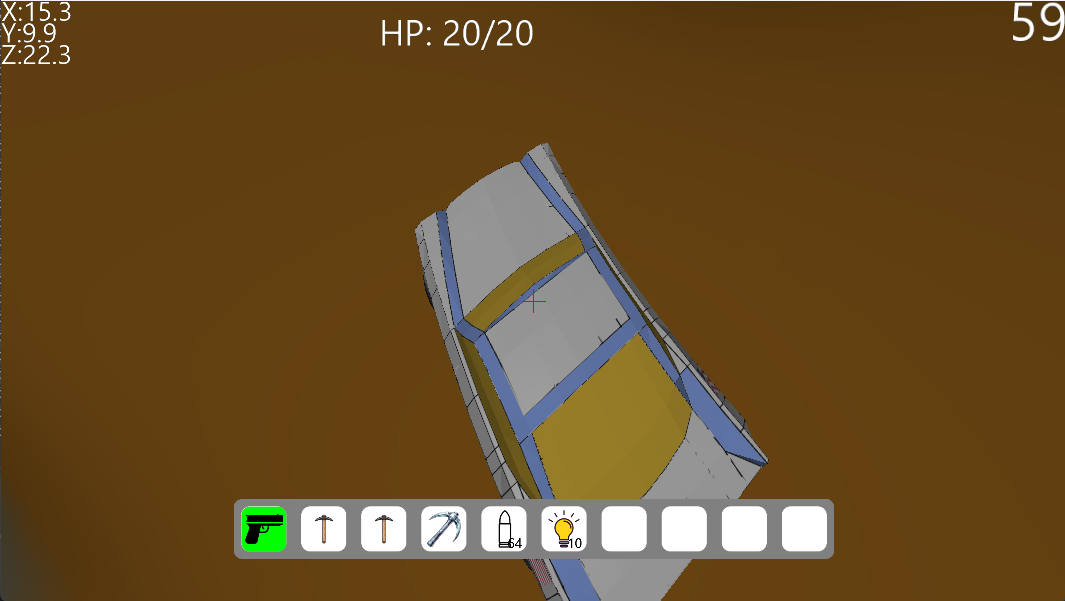
\includegraphics[width=0.6\textwidth]{chapters/theoretical_foundations/sections/non-eudlidean-spaces/resources/bending-car.png}
    \caption{Distrotions caused by porting to spherical space}
    \label{fig:bending-car}
\end{figure}

To minimize the distortions in spherical space we employed the following method.
Due to the periodic nature of the porting given by \autoref{eq:elliptic-porting}, the scene has to be confined inside a 3-dimensional ball of radius $2\pi$.
Since the distortions increase as an object is farther from the origin, we decided to split the scene into two physical regions -- balls of radius $\pi$.
Points $p$ in the first ball (centered at the origin) are mapped to spherical geometry using the mapping
\begin{equation} \label{eq:spherical-port-1}
    \mathcal{P}_{E,1}(p) = (p / \lVert p\rVert \sin(\lVert p\rVert), \cos(\lVert p\rVert))
\end{equation}
and points $p$ in the second ball (which is centered at a point $c$) using the formula
\begin{equation}\label{eq:spherical-port-2}
    \mathcal{P}_{E,2}(p) = (p' / \lVert p' \rVert \sin(\lVert p' \rVert), -\cos(\lVert p'\rVert)),
\end{equation}
where $p' = p - c$.
In the 2-dimensional case, the regions become disks with radii of length $\pi$, and the effect of using \autoref{eq:spherical-port-1} and \autoref{eq:spherical-port-2} can be visualized as "wrapping" the first disk on the upper half of a unit sphere, and "wrapping" the second one on the lower half of the sphere.

Dealing with distortions in hyperbolic space requires a more drastic approach because the scene we wished to port was potentially infinite.
The main goal was to keep the distortions as small as possible near the camera.
To achieve this, the camera position is fixed at some point close to the origin, e.g. $(0, 1, 0)$.
The movement of the camera is then simulated by moving all of the objects in the scene in the direction opposite to the camera's movement direction.
\subsection{Teleporation in spherical space} \label{sub:teleportation}
Even though splitting the scene into two regions in spherical geometry allows us to minimize distortions significantly, it introduces a wide range of other problems.
The most important one has to do with moving objects and the camera from one region to the other; we call this process \textit{teleportation}.

Teleportation is schematically shown in \autoref{fig:teleportation}.
\begin{figure}[h]
    \centering
    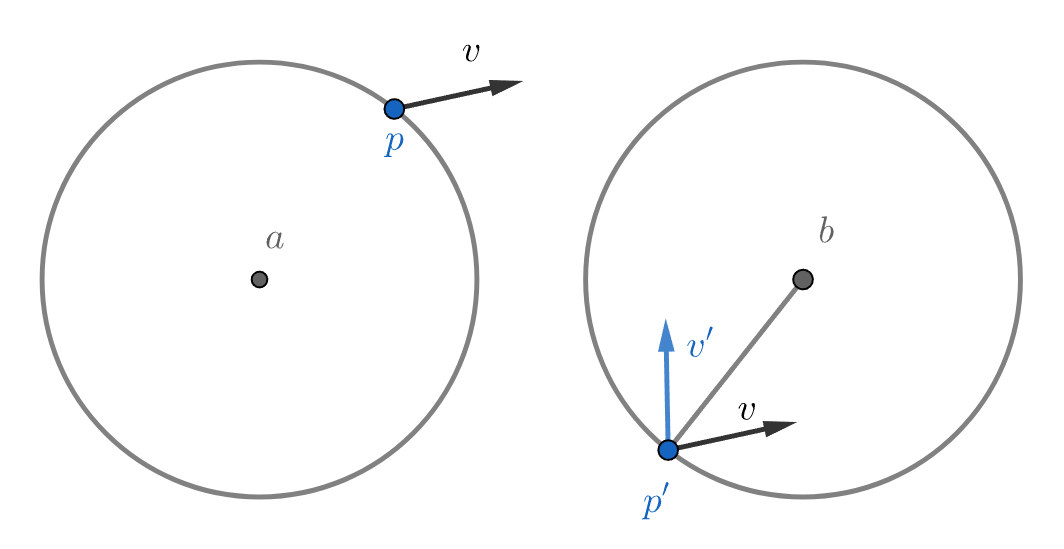
\includegraphics[width=0.6\textwidth]{chapters/theoretical_foundations/sections/non-eudlidean-spaces/resources/teleportation.png}
    \caption{Teleportation between two regions}
    \label{fig:teleportation}
\end{figure}
In this 2-dimensional example, an object leaves the first region (centered at $a$) at the point $p$ and is teleported to the second region (centered at $b$), appearing at a location given by the point $p'$:
\begin{equation*}
    p' = b + R_{xz}(p - a),
\end{equation*}
where $R_{xz}(p)$ denotes reflection of a point $p$ across the origin.
The velocity vector $v$ of the object is mapped to vector $v'$ which is the reflection of $v$ on a vector $p - a$.

The teleportation in the 3-dimensional case can be defined in a very similar manner.
There are only two differences.
The first one is that $R_{xz}(p)$ now denotes a reflection on the unit vector $\hat{y}$ (assuming positive $y$ direction coincides with the "up" direction for the scene).
The second difference is that $v'$ is now the reflection of $v$ through a plane through the origin orthogonal to $(p - a) \times \hat{y}$.

To account for the point reflection $R_{xz}$, the porting given by \autoref{eq:spherical-port-2} has to be modified by replacing $p'$ with $R_{xz}(p')$.

Setting up the view transformation in the second region also comes with its own set of challenges.
The standard way of obtaining the vectors $i'$, $j'$, and $k'$ for the view matrix \ref{eq:view-matrix} is as follows.
We first port the camera position to non-Euclidean space (in the case of the second region, we use \autoref{eq:spherical-port-2}), and then use the \autoref{eq:porting-vector} to port its right, up, and front vectors.
The problem with this approach is that the translation matrix \ref{eq:translation-matrix} is defined in terms of translating the geometry origin $g = (0, 0, 0, 1)$ and not $(0, 0, 0, -1)$.
This means that if the translation target $q$ is close to $(0, 0, 0, -1)$, $T(q)$ can map a point $p$ with $p_w < 0$ to a new point $p'$ with $p'_w > 0$ because
\begin{equation*}
    p'_w = -q_x p_x - q_y p_y - q_z p_z + q_w p_w \approx q_w p_w > 0.
\end{equation*}
The matrix isn't even defined for translation targets with $q_w = -1$.

To solve this problem, we derived a translation matrix $T_2(q)$ which we use for translations in the second region.
It is defined analogously to $T(q)$ given by \autoref{eq:translation-matrix}, but in the context of $T_2$, the translation target $q$ is the point that the point $(0, 0, 0, -1)$ is translated to.
The matrix is given by
\begin{equation}
    T_2(q) = \begin{bmatrix}
        1 - \frac{q_x^2}{1 - q_w} & -\frac{q_x q_y}{1 - q_w}  & -\frac{q_x q_z}{1 - q_w}  & q_x  \\
        -\frac{q_y q_x}{1 - q_w}  & 1 - \frac{q_y^2}{1 - q_w} & -\frac{q_y q_z}{1 - q_w}  & q_y  \\
        -\frac{q_z q_x}{1 - q_w}  & -\frac{q_z q_y}{1 - q_w}  & 1 - \frac{q_z^2}{1 - q_w} & q_z  \\
        -q_x                      & -q_y                      & -q_z                      & -q_w
    \end{bmatrix}.
\end{equation}
Using the fact that $q$ is in the spherical geometry, i.e. $\langle q, q \rangle_E = 1$, it can be verified that the row vectors of the matrix are orthonormal, thus the matrix describes an isometry.
Moreover, $T_2((0, 0, 0, -1))$ is the identity matrix as expected.
\section{Marching Cubes} \label{sec:theory_theory_marching_cubes}
One of the requirements for our project was to incorporate terrain generation.
Numerous algorithms exist for this purpose, and the chosen algorithm for our project is known as marching cubes.
This algorithm was selected due to its simplicity, versatility, and standardization.
Marching cubes is a relatively straightforward algorithm that can be easily modified to suit different requirements, as explained in detail in \autoref{sec:system_architecture_terrain_generation}.
Furthermore, it is widely used in various applications and is well-documented, making its understanding and implementation easier.

The concept of marching cubes was first introduced by William E. Lorensen and Harvey E. Cline in 1987 \cite{Marching-Cubes}.
The fundamental idea behind this algorithm is to generate a mesh from a scalar field.
An isolevel is chosen, 0 being the most common choice and the one we used.
Points with values greater than the isolevel are considered to be "above" the surface, while points with values lower than the isolevel are considered to be "below" the surface.
The world is divided into cubes, and for each cube, the algorithm determines which of its vertices are above and below the surface.
Based on this information, a mesh is created to separate the vertices above the surface from those below it.
An example of this process is illustrated in \autoref{fig:cube_example}, where $v0$ is below the surface, while the remaining vertices are above it.
It is important to note that the same effect would be achieved if $v0$ were above the surface and the other vertices were below it.

\todo{Can we use images found online? If so how do we cite them?}
\begin{figure}[H]
    \centering
    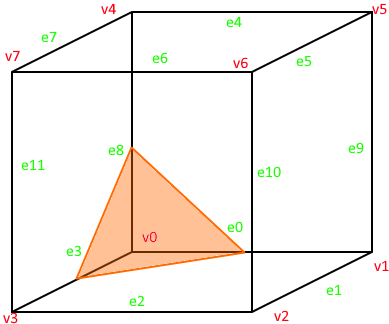
\includegraphics[width=0.5\textwidth]{chapters/theoretical_foundations/sections/marching_cubes/resources/cube-example.png}
    \caption["Marching" cubes with only $v0$ below the surface.]{"Marching" cubes with only $v0$ below the surface. Source: \url{https://polycoding.net/marching-cubes/}}
    \label{fig:cube_example}
\end{figure}

Each cube consists of 8 vertices, and each vertex is classified as either above or below the surface, resulting in a total of 256 possible combinations.
However, there are only 15 unique combinations, all of them depicted in \autoref{fig:marching_cubes_configurations}, with the remaining combinations being rotations and reflections of these 15 cases.
For each of these unique combinations, a precomputed table is utilized to generate the corresponding mesh.
This table provides information about which edges of the cube are intersected by the surface and how to connect them.

\begin{figure}[H]
    \centering
    
\includegraphics[width=0.8\textwidth]{chapters/theoretical_foundations/sections/marching_cubes/resources/marching-cubes-configurations.png}
    \caption[Unique marching cubes configurations]{Unique marching cubes configurations. Source: \url{https://polycoding.net/marching-cubes/}}
    \label{fig:marching_cubes_configurations}
\end{figure}

\chapter{System Architecture} \label{ch:system_architecture}
This section describes the system architecture of the game.
\section{Terrain} \label{sec:system_architecture_terrain}
The terrain was designed to be randomly generated so that the player can have a new, unique map every time they play.
The second important part of the design was making sure that the player could edit the terrain in any way they wanted.
As described in \autoref{sec:theory_theory_marching_cubes} the marching cubes algorithm was chosen as the base of the terrain generation process.
This section will describe how we used this algorithm to generate the terrain and allow the player to edit it.

The algorithm consists of the following steps:
\begin{itemize}
    \item Define the scalar field function.
    \item Divide the world into chunks.
    \item Generate the mesh.
\end{itemize}

Each of these steps will be described in detail in this section.

\subsection{Scalar Field} \label{subsec:scalar_field}
The first step in the terrain generation is to generate a scalar field which is a function that takes a point in 3D space and returns a value.
What is important is that this function always returns the same value for the same point.
Another important property is that the function should return close values for close points.
Our function returns values for points that have integer coordinates.

Having these properties in mind we decided to use the Perlin noise function.
Perlin noise first introduced by Ken Perlin in 1983 \cite{Perlin-Noise} is often used in computer graphics and in particular in procedural terrain generation.
It is a pseudo-random function that returns values for any point in 3D space.
\question{Should we explain how the Perlin noise function works? Our implementation does not add anything to it.}
However, unlike some random functions, it returns similar values for similar points.
This makes it ideal for this game.

The Perlin noise function is used to generate a value for each point in the scalar field.
This value is then modified based on 5 parameters: octaves, initial frequency, frequency multiplier, initial amplitude and amplitude multiplier.
How these parameters affect the terrain can be seen in \autoref{fig:argument_comparison}.
These parameters are generated based on the seed of the world from 5 different sets of options which gives the game 5 terrains.
However, we need more than just the value for each point and a normal vector.
Each point is also assigned a type based on the position that is later used to determine the type of the block which in turn determines its color.

\newpage
\begin{figure}[h]
    \centering
    \begin{subfigure}{0.45\textwidth}
        \centering
        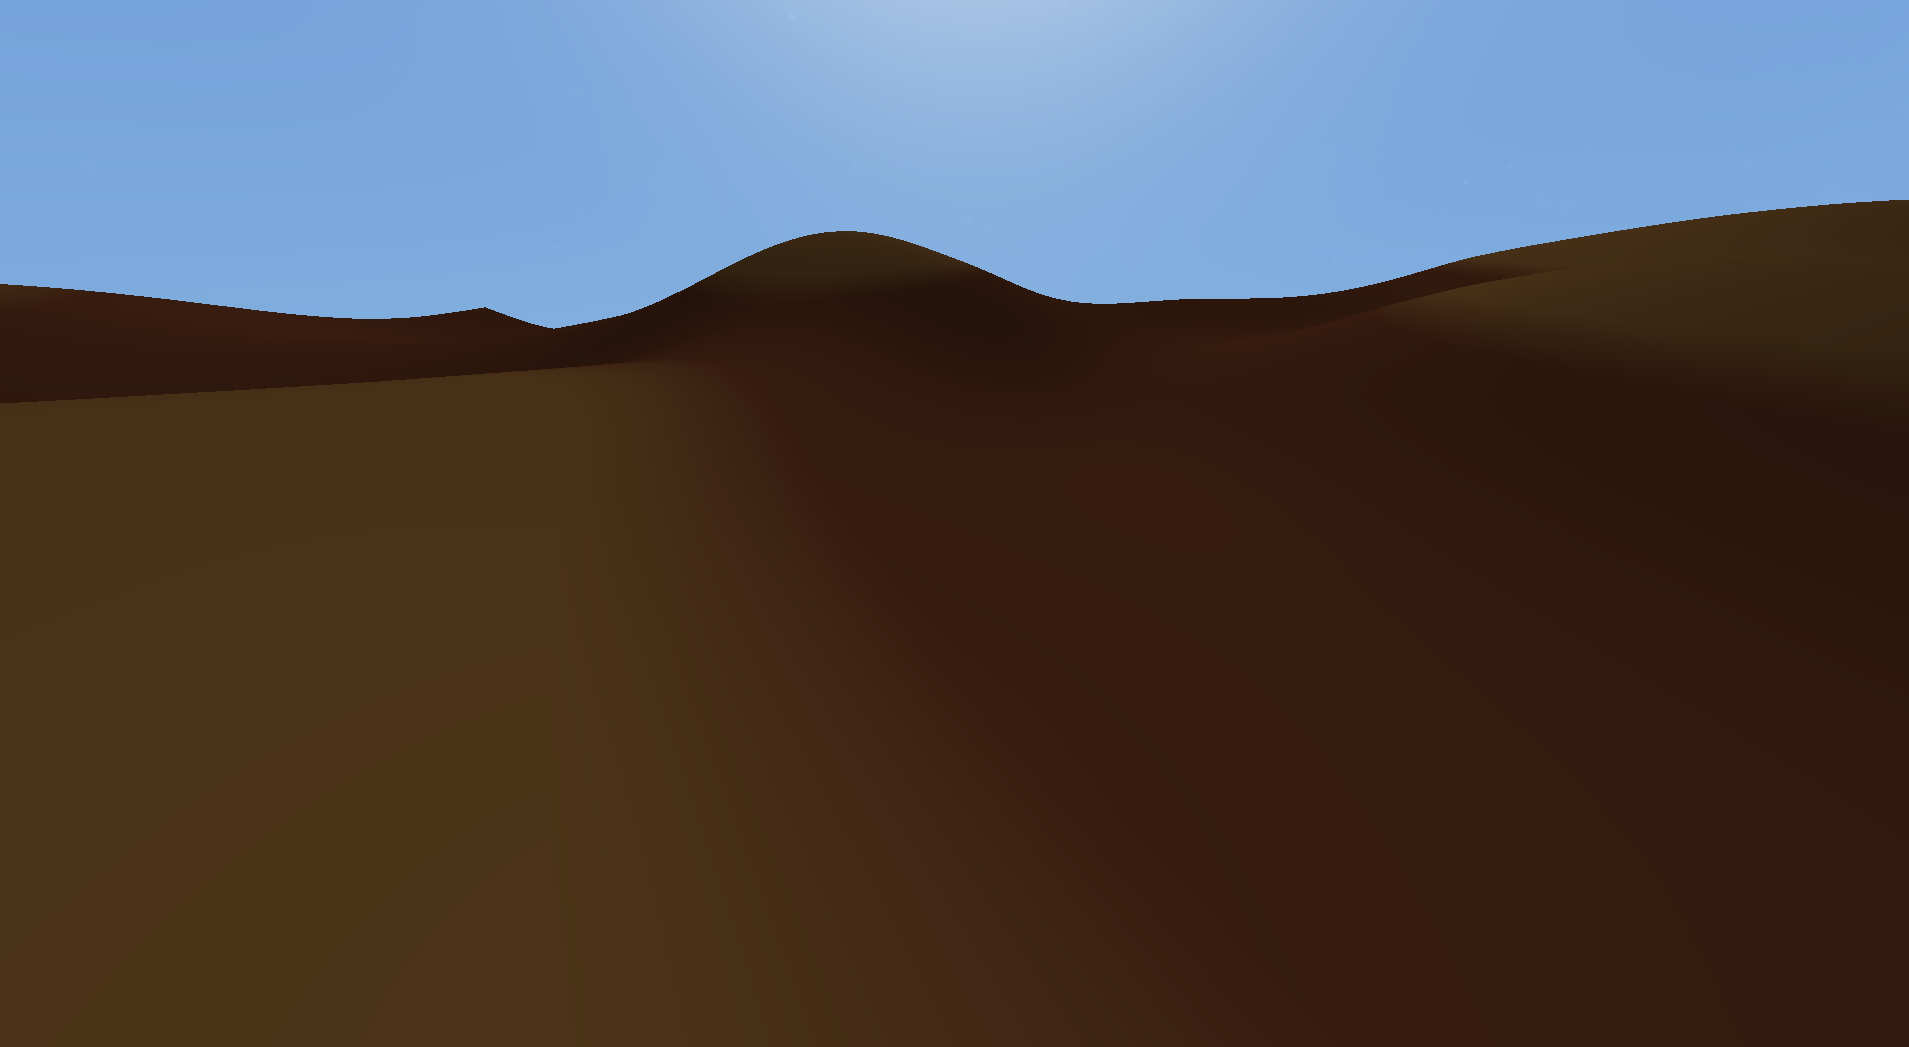
\includegraphics[width=0.8\textwidth]{chapters/system_architecture/sections/terrain/resources/octaves-1.png}
        \caption{Small octaves (1).}
    \end{subfigure}
    \hfill
    \begin{subfigure}{0.45\textwidth}
        \centering
        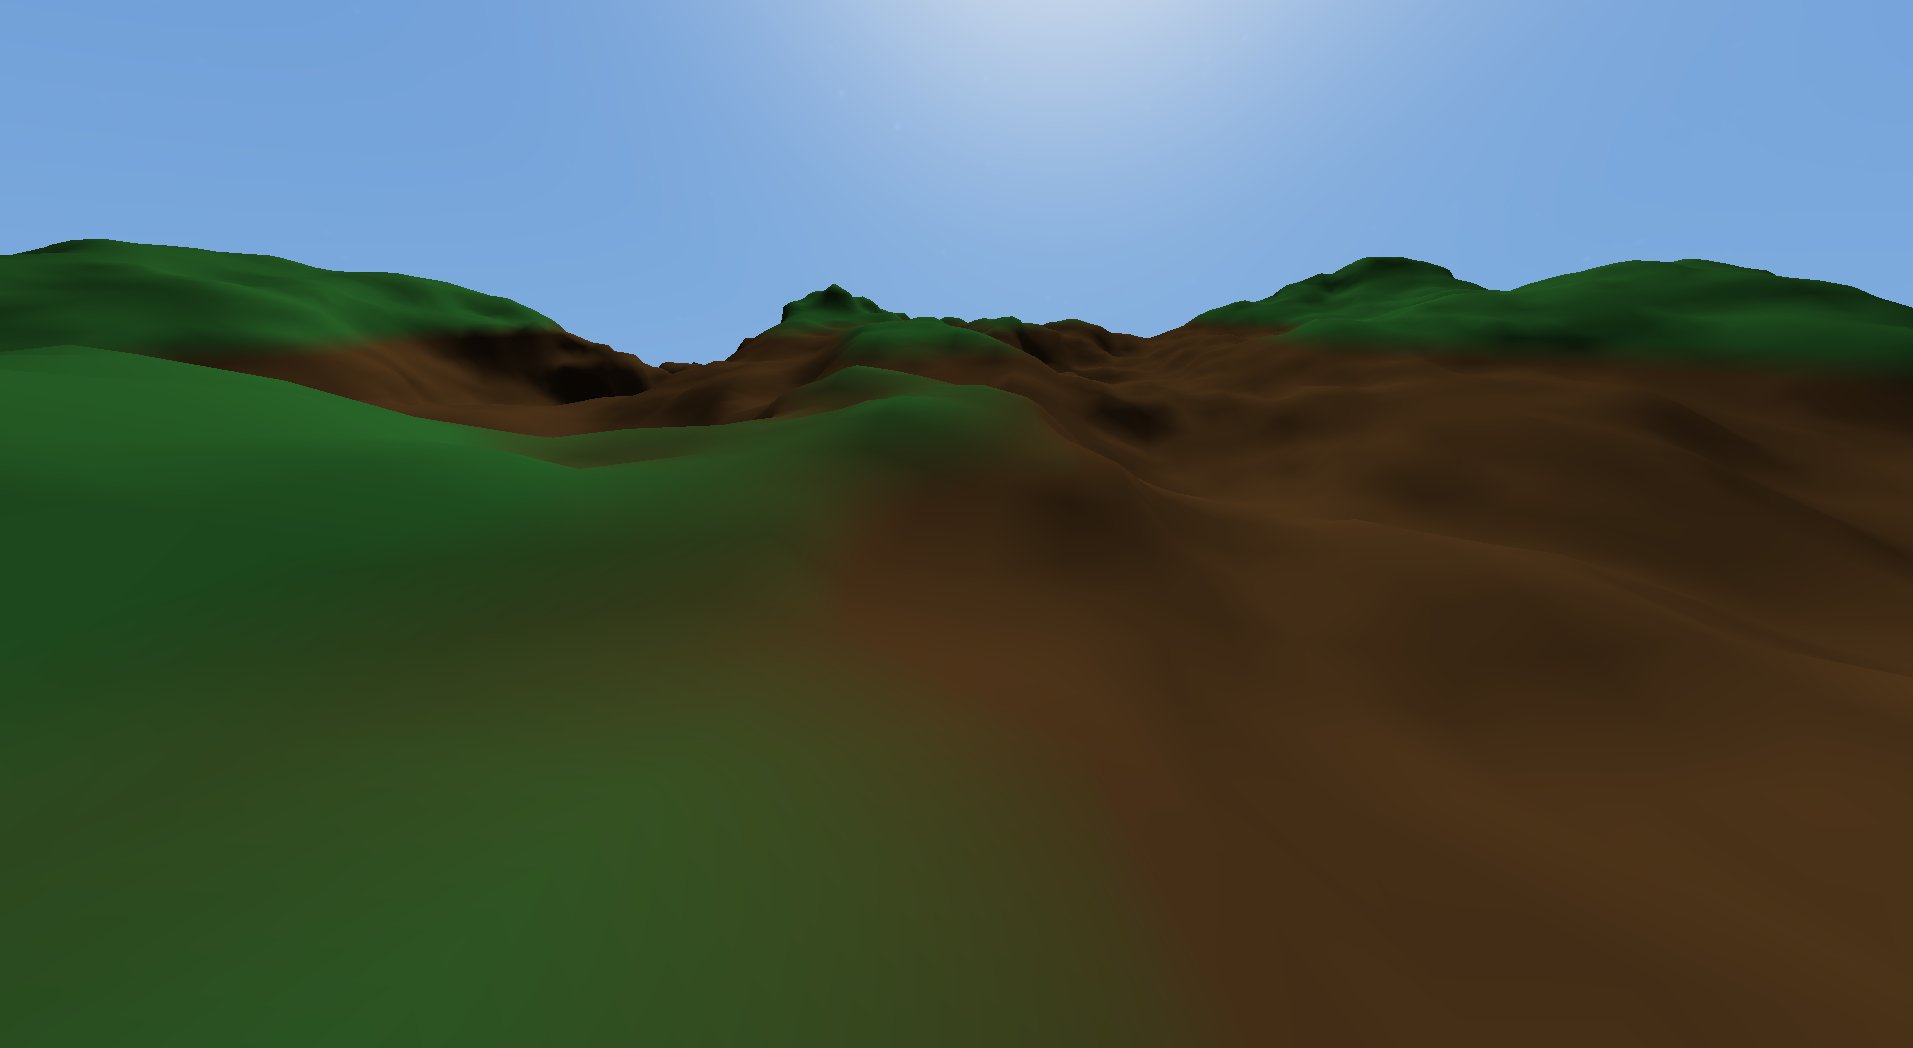
\includegraphics[width=0.8\textwidth]{chapters/system_architecture/sections/terrain/resources/octaves-5.png}
        \caption{Big octaves (5).}
    \end{subfigure}

    \centering
    \begin{subfigure}{0.45\textwidth}
        \centering
        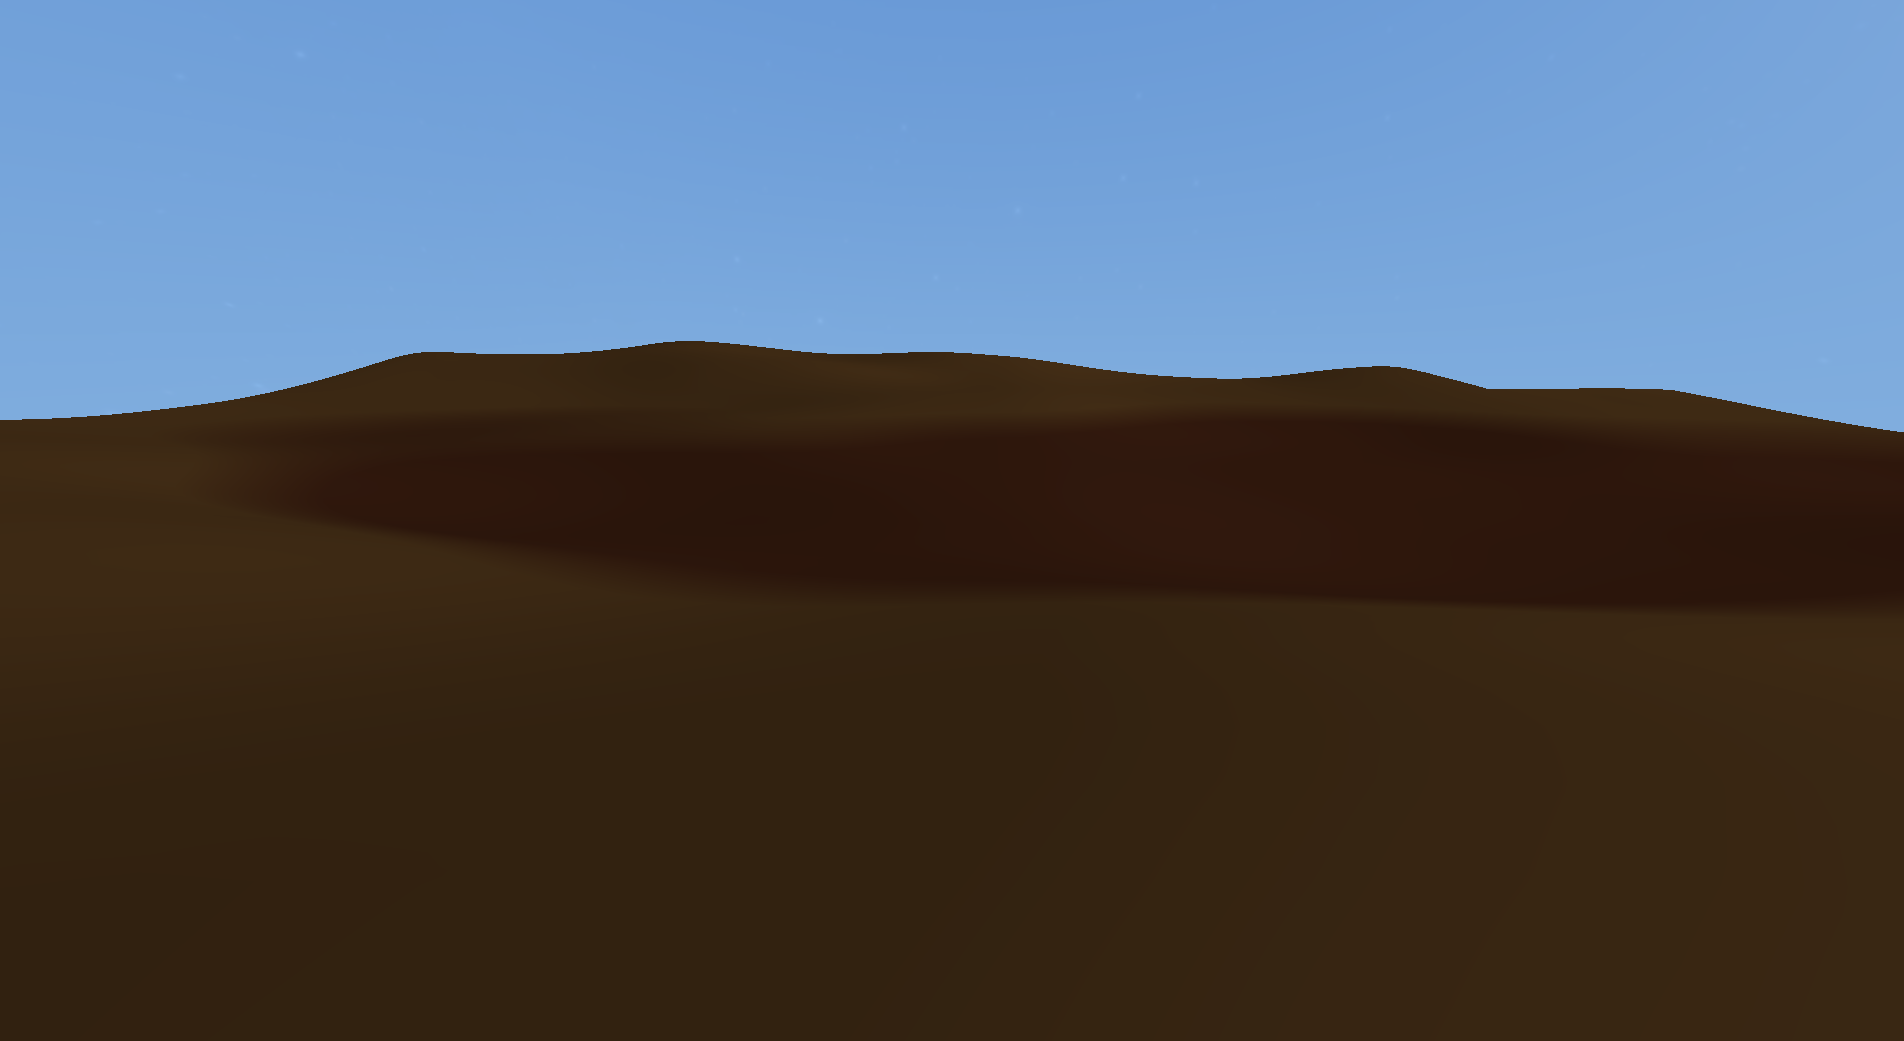
\includegraphics[width=0.8\textwidth]{chapters/system_architecture/sections/terrain/resources/initial-freq-0.1.png}
        \caption{Small initial frequency (1).}
    \end{subfigure}
    \hfill
    \begin{subfigure}{0.45\textwidth}
        \centering
        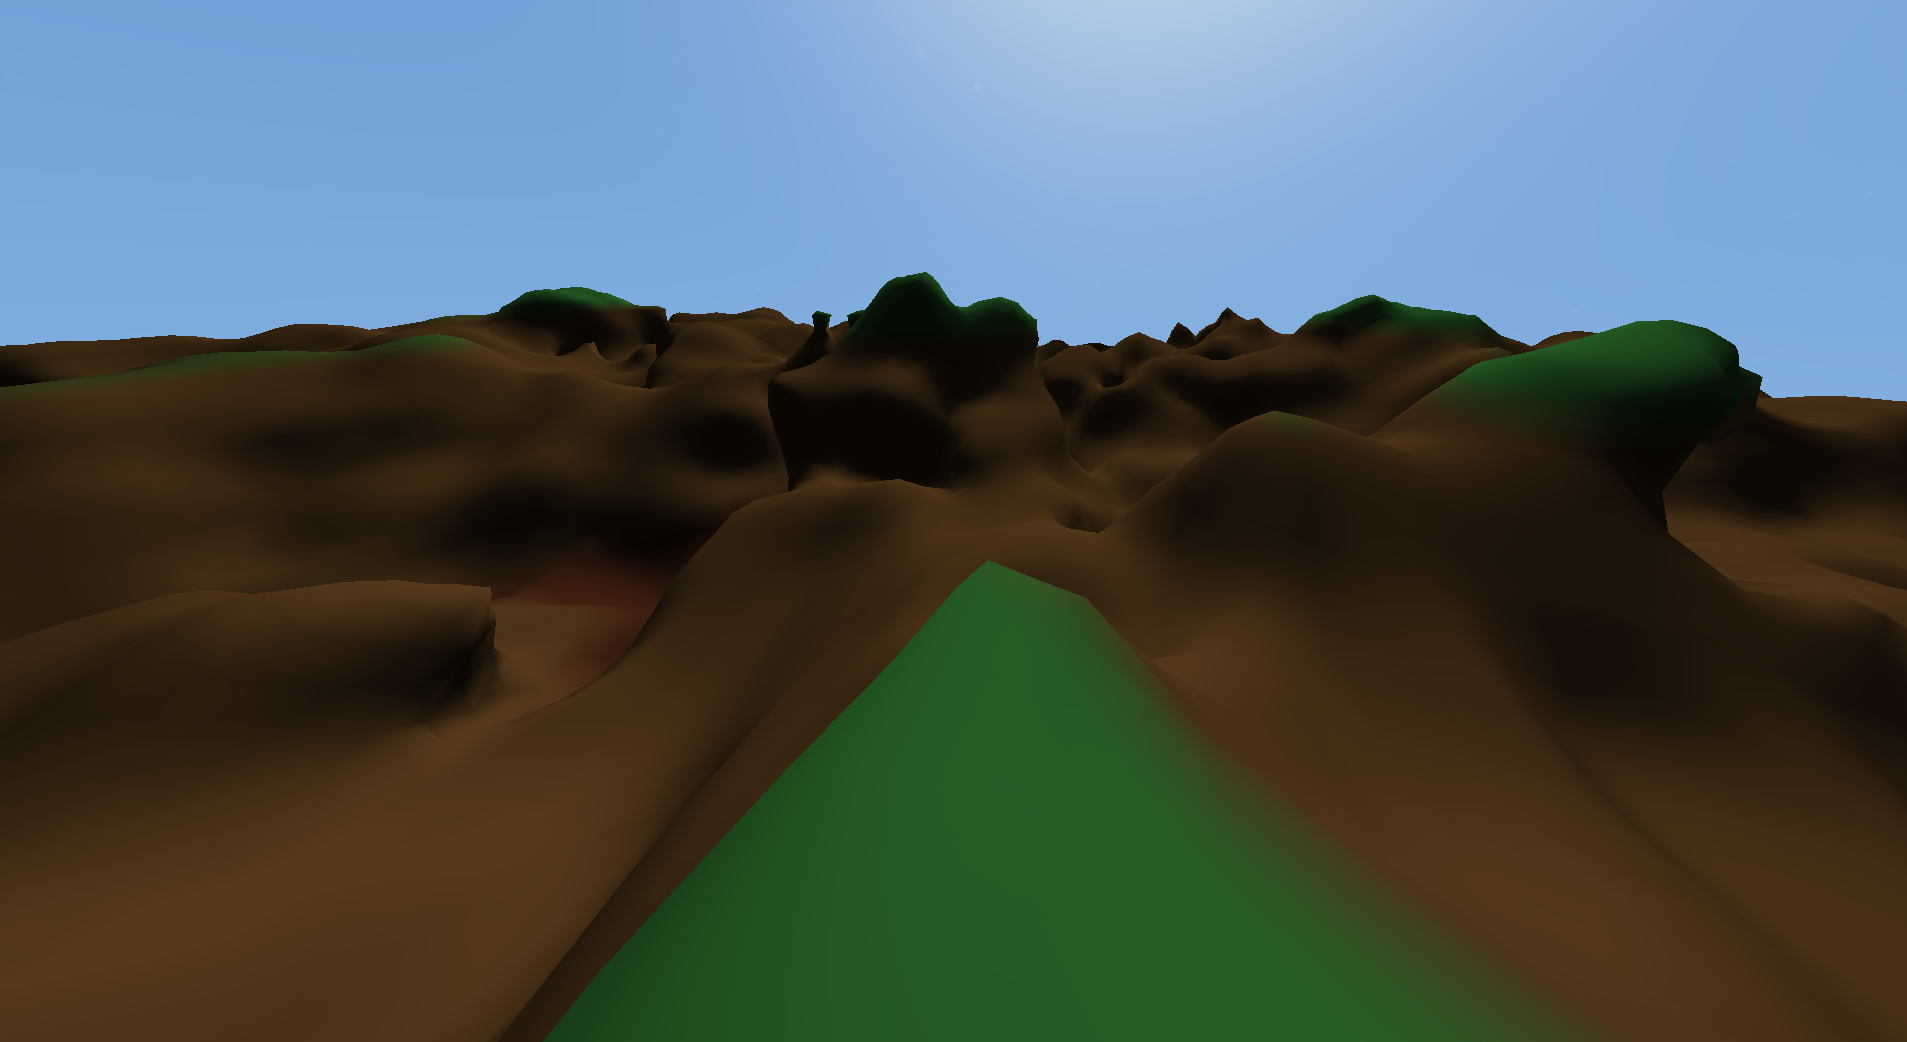
\includegraphics[width=0.8\textwidth]{chapters/system_architecture/sections/terrain/resources/initial-freq-0.5.png}
        \caption{Big initial frequency (0.5).}
    \end{subfigure}

    \centering
    \begin{subfigure}{0.45\textwidth}
        \centering
        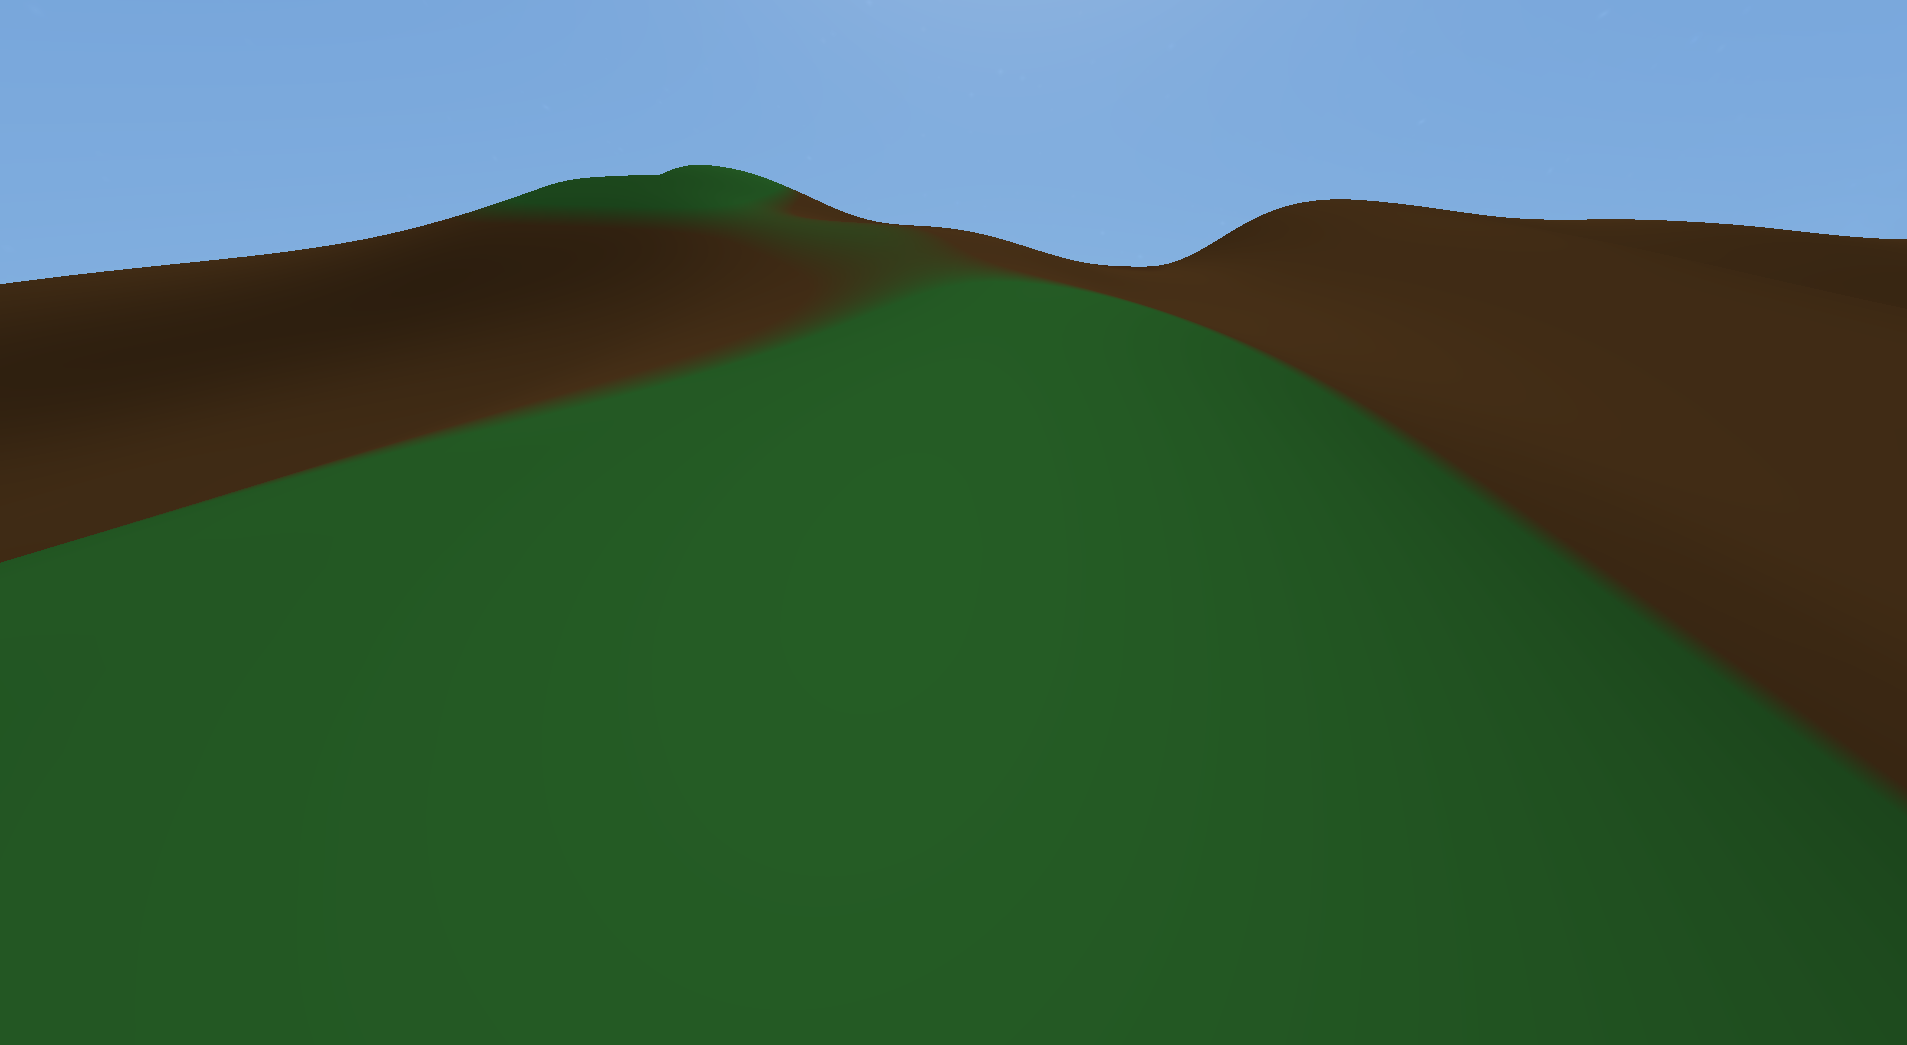
\includegraphics[width=0.8\textwidth]{chapters/system_architecture/sections/terrain/resources/freq-mul-0.5.png}
        \caption{Small frequency multiplier (0.5).}
    \end{subfigure}
    \hfill
    \begin{subfigure}{0.45\textwidth}
        \centering
        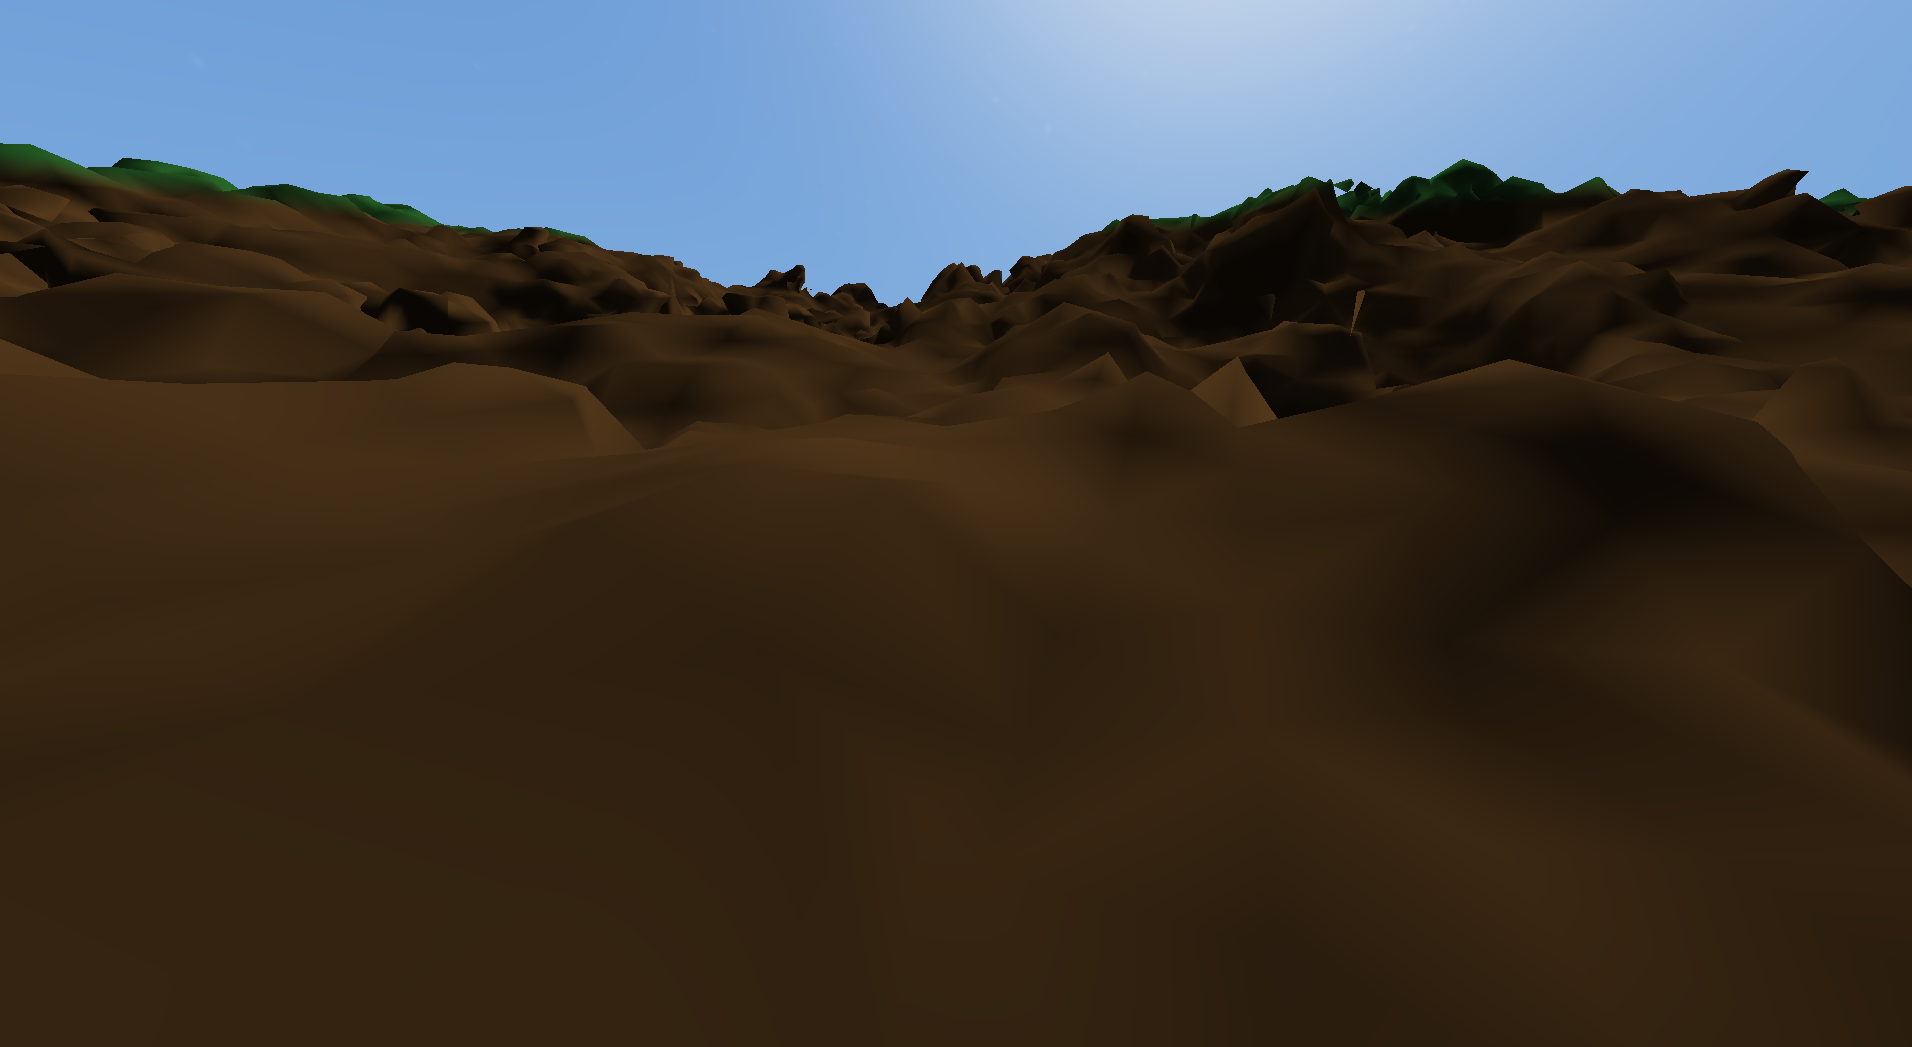
\includegraphics[width=0.8\textwidth]{chapters/system_architecture/sections/terrain/resources/freq-mul-5.png}
        \caption{Big frequency multiplier (5).}
    \end{subfigure}

    \centering
    \begin{subfigure}{0.45\textwidth}
        \centering
        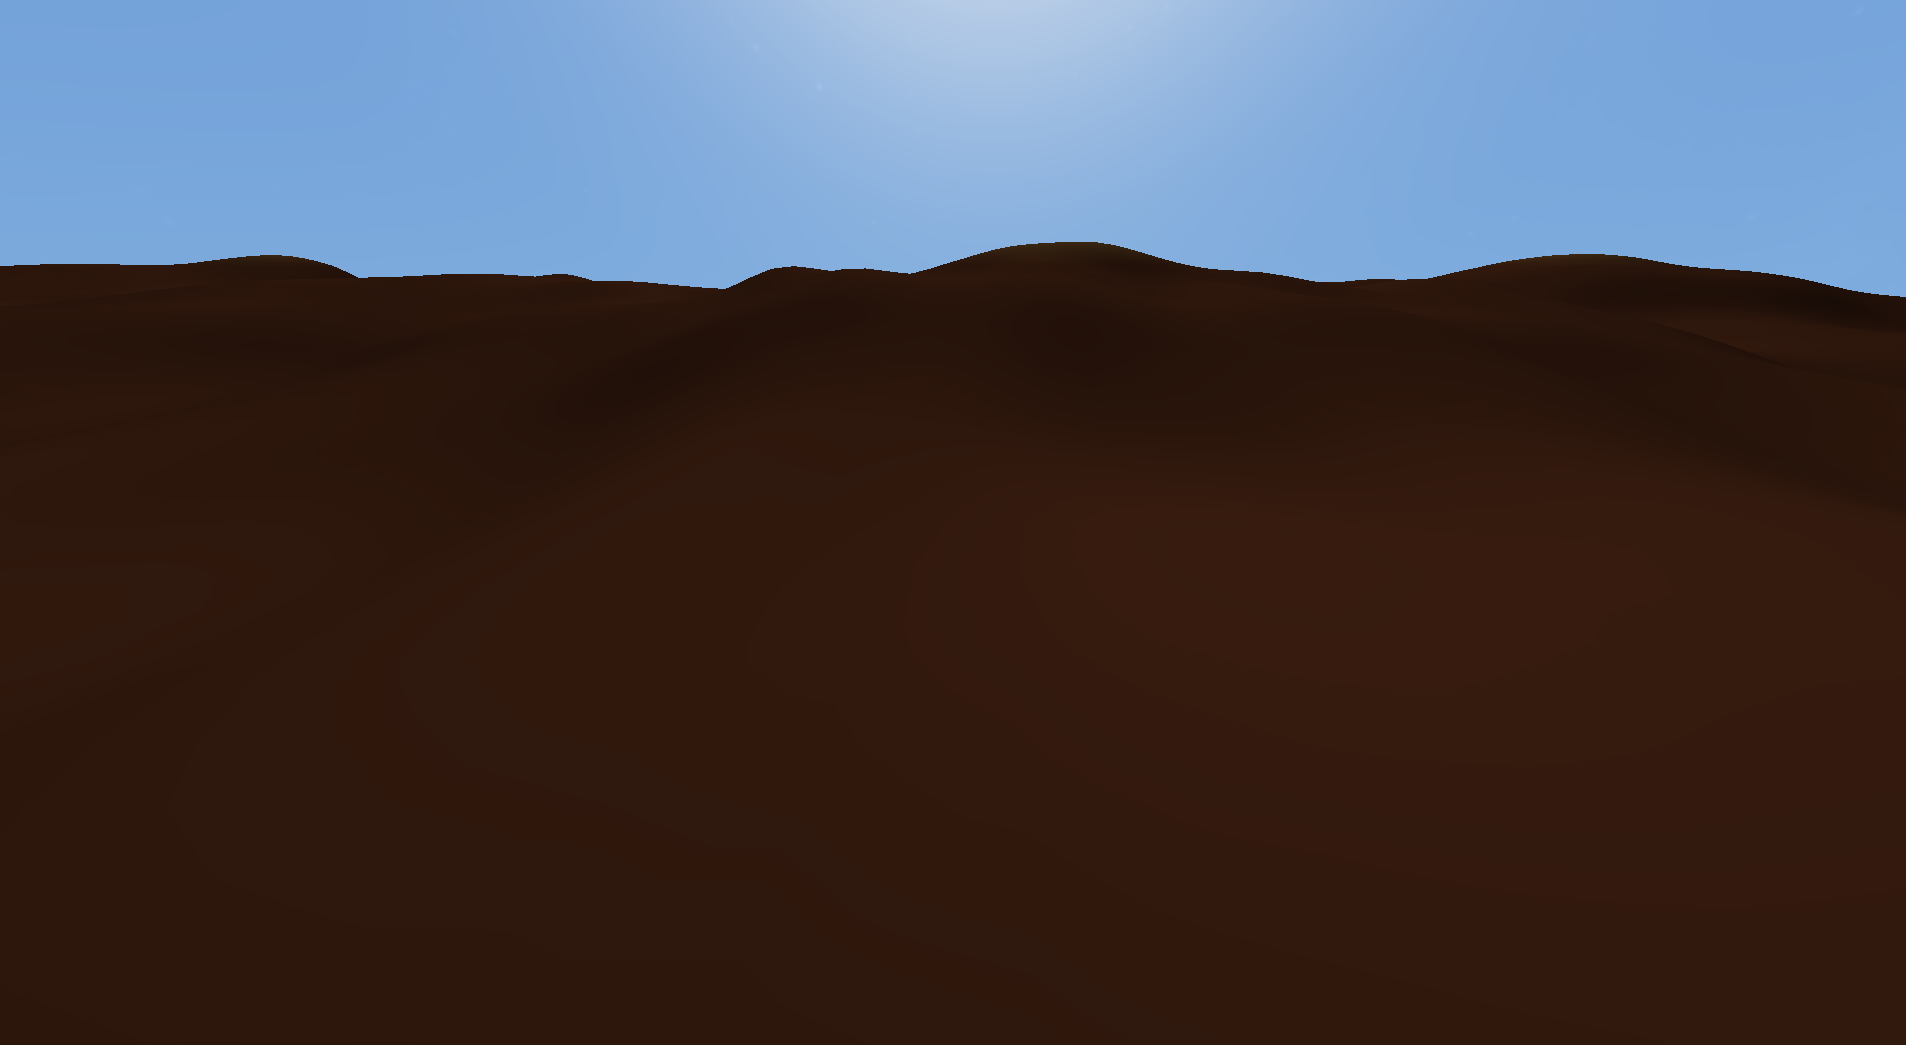
\includegraphics[width=0.8\textwidth]{chapters/system_architecture/sections/terrain/resources/initial-amp-8.png}
        \caption{Small initial amplitude (8).}
    \end{subfigure}
    \hfill
    \begin{subfigure}{0.45\textwidth}
        \centering
        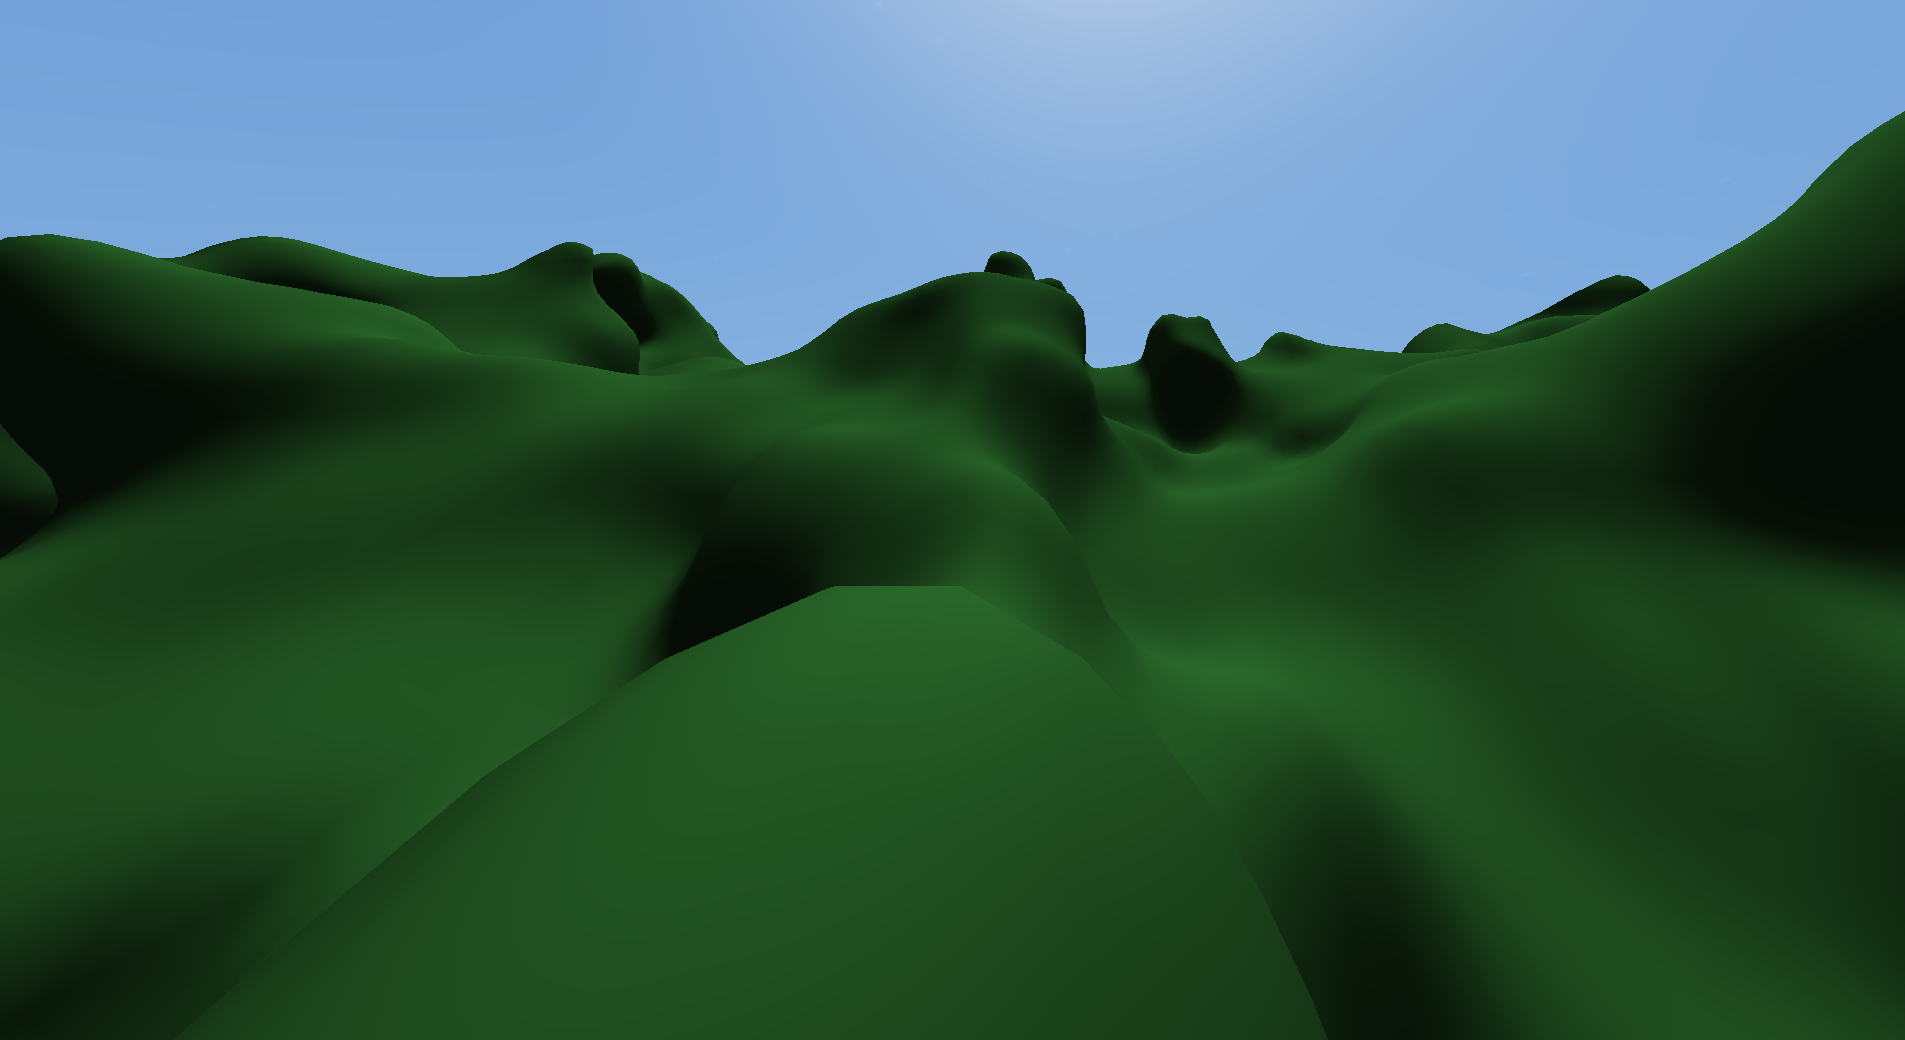
\includegraphics[width=0.8\textwidth]{chapters/system_architecture/sections/terrain/resources/initial-amp-32.png}
        \caption{Big initial amplitude (32).}
    \end{subfigure}

    \centering
    \begin{subfigure}{0.45\textwidth}
        \centering
        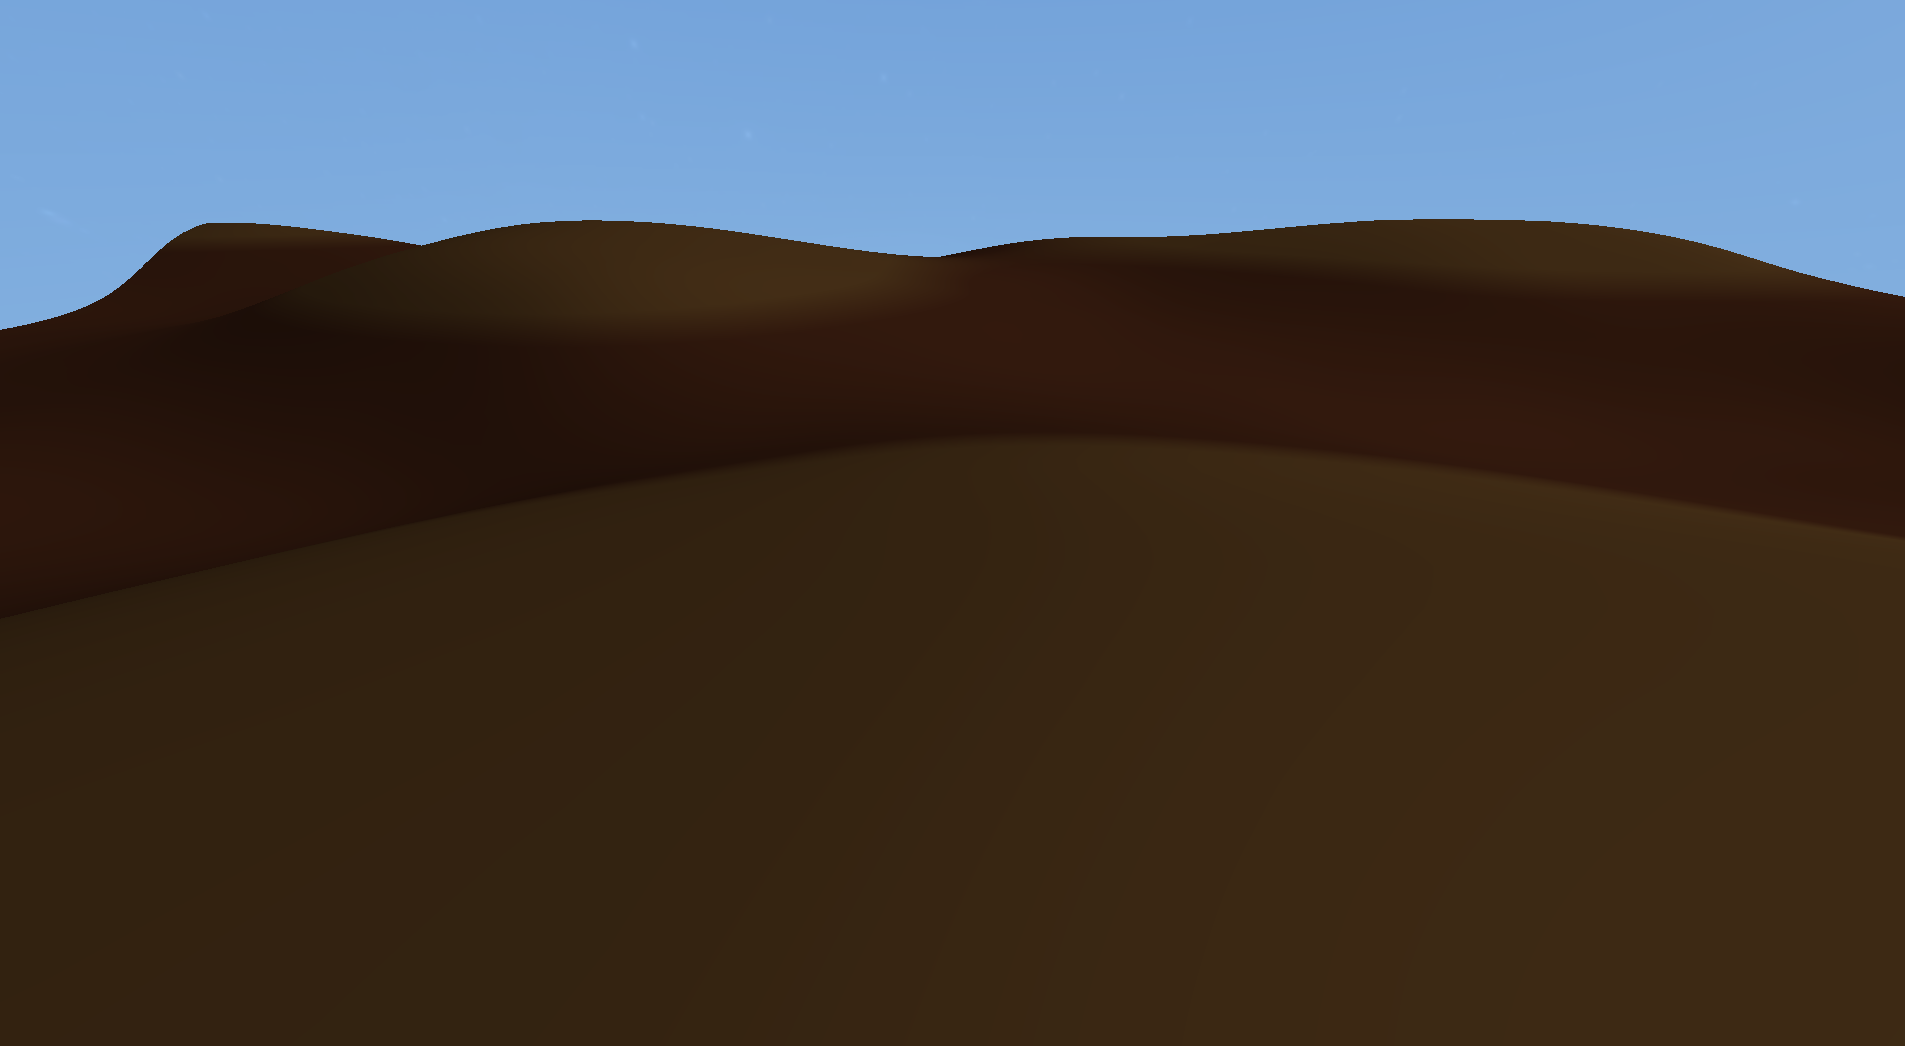
\includegraphics[width=0.8\textwidth]{chapters/system_architecture/sections/terrain/resources/amp-mul-0.1.png}
        \caption{Small amplitude multiplier (0.1).}
    \end{subfigure}
    \hfill
    \begin{subfigure}{0.45\textwidth}
        \centering
        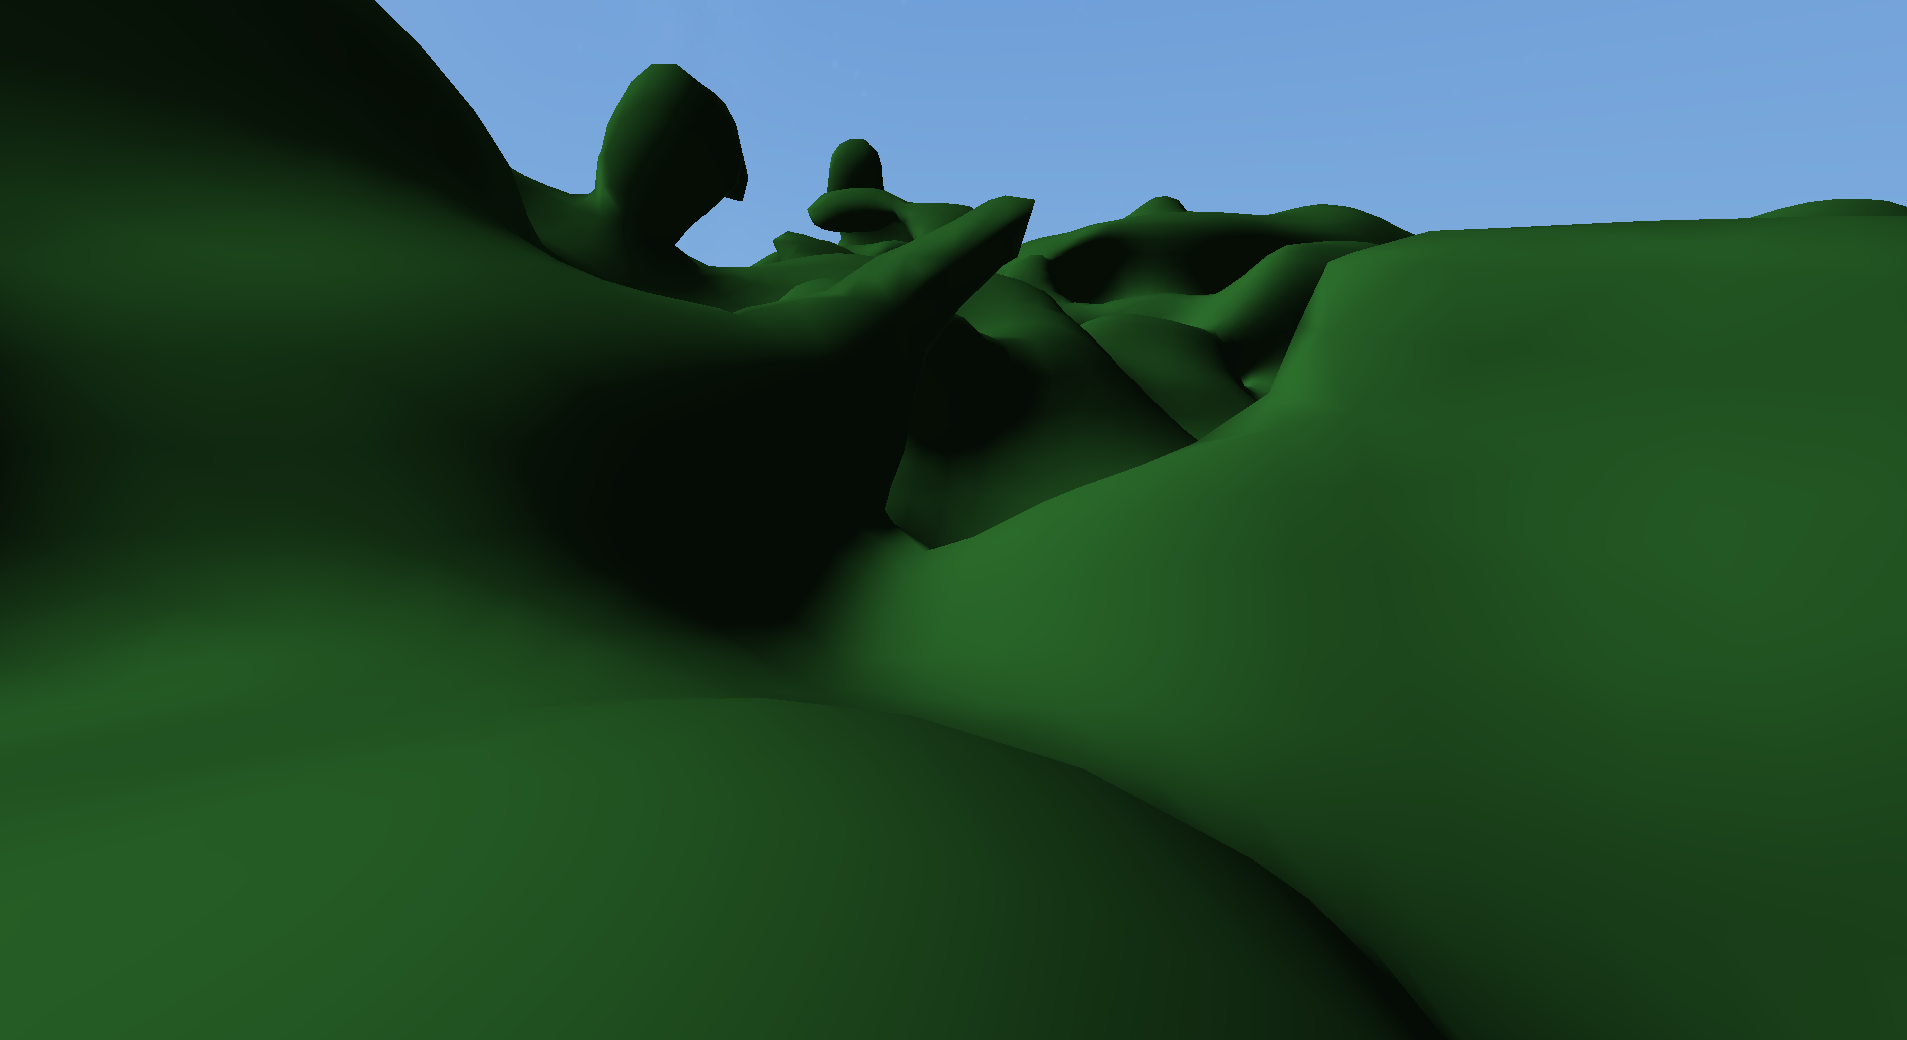
\includegraphics[width=0.8\textwidth]{chapters/system_architecture/sections/terrain/resources/amp-mul-1.png}
        \caption{Big amplitude multiplier (1).}
    \end{subfigure}

    \caption{Scalar field parameter comparison.}
    \label{fig:argument_comparison}
\end{figure}
\subsection{Chunks}
As mentioned before one of the most important things for the terrain was a way to edit it.
Editing the whole terrain at once would be very slow and not very efficient.
Thus the terrain is split into chunks - cubes with side length 16.
Each chunk is a separate object and can be edited independently.
This solution is much more efficient but it also causes some problems.

One problem is that the terrain is not continuous.
Every time we edit a chunk we need to make sure that the edges of the chunk are the same as the edges of the neighboring chunks.
This is done by making sure that when a function that updates one chunk is called it is also called with the same parameters for other affected chunks.
Without this, the terrain would have holes in it between chunks which is shown in a screenshot from an early version of the game in \autoref{fig:gaps_between_chunks}.

Another problem is that the algorithm we used for generating the terrain, described in \autoref{subsec:marching_cubes}, calculates normal vectors based on the values of the scalar field around the point at which the normal is calculated.
This means that the normal vectors at the edges of the chunks have to be calculated differently.
This is a common problem with the algorithm and it is visualized in \autoref{fig:problem_with_normals_at_chunk_edge}.
The most common solution and the one we used is extending the scalar field by one layer of points around the chunk.
This means that the chunk contains information about the scalar field outside of the chunk itself.
That way the normal vectors can be calculated the same way for all points in the chunk.

\begin{figure}[H]
    \centering
    \begin{minipage}{0.45\textwidth}
        \centering
        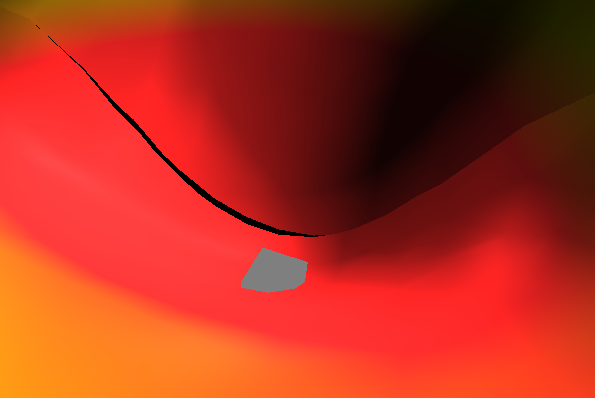
\includegraphics[width=0.8\textwidth]{chapters/system_architecture/sections/terrain/resources/chunk_edges_gaps.png}
        \caption{Gaps between chunks.}
        \label{fig:gaps_between_chunks}
    \end{minipage}\hfill
    \begin{minipage}{0.45\textwidth}
        \centering
        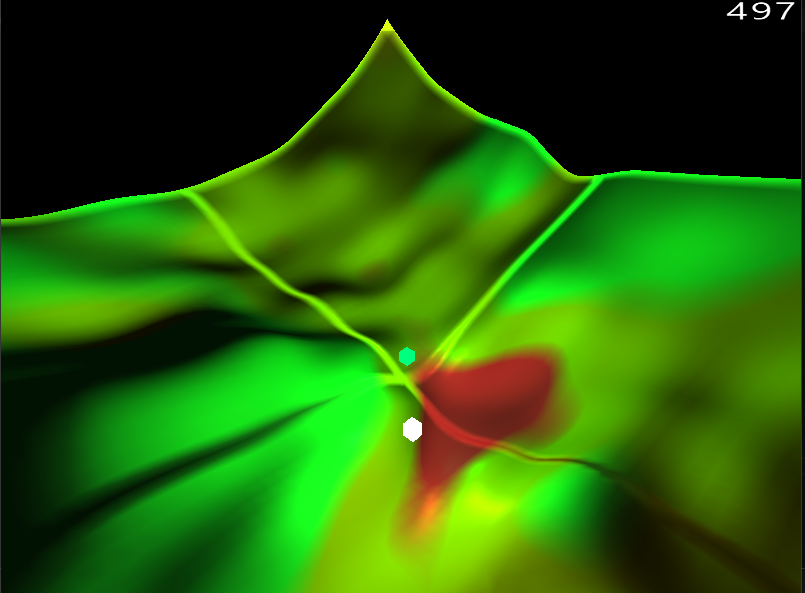
\includegraphics[width=0.8\textwidth]{chapters/system_architecture/sections/terrain/resources/chunk_edges_normals_problem.png}
        \caption{Problem with normals at chunk edges.}
        \label{fig:problem_with_normals_at_chunk_edge}
    \end{minipage}
\end{figure}

There are infinitely many chunks in the world, which is why chunks are only loaded when a player is close to them.
They are also unloaded when the player moves far enough away from them.
When that happens they are saved to disk and removed from RAM.
The same thing happens when the game is closed.
\subsection{Marching Cubes} \label{subsec:marching_cubes}
The idea of the algorithm is described in \autoref{sec:theory_theory_marching_cubes}.
This section will describe the way the algorithm was implemented in our project.

To make the mesh look smoother we interpolate the position of the vertices on the edges based on the values of the scalar field at the vertices.
This is done by using the linear interpolation given by equation \autoref{eq:linear_interpolation}.
\begin{equation}
  \label{eq:linear_interpolation}
  P = V_1 + \frac{\text{IsoLevel} - v_1}{v_2 - v_1} \times (V_2 - V_1)
\end{equation}
where $P$ is the resulting position of the vertex, $V_1$ and $V_2$ are the positions of the vertices on the edge, $v_1$ and $v_2$ are the values of the scalar field at the vertices and IsoLevel is the isolevel of the mesh.
  
This gives us a mesh.
To make the impression of a light reflecting off a smooth surface we also need to calculate the normal vectors for each vertex.
The normal vectors for each vertex of the scalar field are calculated using \autoref{eq:normal_vector}
\begin{equation}
    \label{eq:normal_vector}
    n(x, y, z) = \begin{bmatrix}
        s(x + 1, y, z) - s(x - 1, y, z) \\
        s(x, y + 1, z) - s(x, y - 1, z) \\
        s(x, y, z + 1) - s(x, y, z - 1)
      \end{bmatrix}
\end{equation}
where $s(x, y, z)$ is the scalar field function and $n$ is the normal vector.
These vectors are used to calculate the mesh normals using the same interpolation used for the mesh \autoref{eq:linear_interpolation}.

The last part of creating the mesh is assigning the colors to each vertex.
Each vertex of the scalar field is assigned a type which is described in \autoref{subsec:scalar_field}.
Each type has a color assigned to it.
The color of each vertex of the mesh is calculated by interpolating the colors of the vertices of the scalar field using \autoref{eq:linear_interpolation}.


\subsection{Editing terrain} \label{sec:terrain_editing}
Editing terrain is done by changing the values of the scalar field.
When a chunk is first created the values of the scalar field are calculated for each point in the chunk and then saved.
This allows for the scalar field values to be edited.
When a chunk is edited the values of the scalar field are recalculated for the edited points and the points around them.
The player can choose a point to build or mine at.
Values of the scalar field close to that point are then changed based on the pickaxe the player uses and how long they mine for.
The closer the point to the chosen point the more it is affected.
A 3D Gaussian function is used to calculate exactly how much each point is affected.
The function is shown in \autoref{eq:gaussian}.

\begin{equation}
    \label{eq:gaussian}
    f(x,y,z) = e^{-a \left((p_x - c_x)^2 + (p_y - c_y)^2 + (p_z - c_z)^2\right)}
\end{equation}

In \autoref{eq:gaussian} $p_x$, $p_y$ and $p_z$ are the coordinates of the point being edited, $c_x$, $c_y$ and $c_z$ are the coordinates of the chosen point and $a$ is a constant.
Moreover, if the distance between the chosen point and the point being edited is greater than the range of the pickaxe, the point is not affected.

Once the values of the scalar field are updated the chunk is regenerated.
This is a very time-consuming process which is why it was moved to a second thread.
The communication between that thread and the main one is described in: \todo{Describe chunk worker}

\section{Chunk worker} \label{sec:chunk-worker}
The majority of the game logic is handled by a single thread.
The only two exceptions are the physics engine (external library) and the chunk management system.
The chunk management system is split between two threads: the main thread (the thread that the rest of the application is running on) and the \textit{chunk worker's} thread.
The worker's thread is concerned with operations that are either CPU-intensive or could take a long time to execute.
More specifically, the chunk worker is performing the following operations:
\begin{enumerate}
    \item loading saved chunks from disk and generating new chunks,
    \item saving chunks to disk,
    \item updating chunks.
\end{enumerate}
The system is built around the producer-consumer pattern, i.e. the main thread communicates with the worker's thread (and \textit{vice versa}) using queues.
It's important to note that depending on the stage of an operation either thread can be the \textit{producer} or the \textit{consumer}.
We will now describe the workflow for each of the operations mentioned before.

\subsection{Loading and generating chunks}
On each render frame, the main thread calls the \texttt{UpdateCurrentPosition} method.
This method, based on the camera's current position and the render distance, determines which chunks should be loaded into the game.
If a chunk isn't already loaded or isn't queued for loading, the position of the chunk is enqueued into the \texttt{chunksToLoad} queue.

The worker thread in the \texttt{LoadChunks} function dequeues the positions of the chunks to be loaded from the disk.
If a chunk is not saved on the disk, it is generated.
The loaded/generated chunk is then enqueued into the \texttt{loaded} queue.

The main thread through the \texttt{ResolveLoaded} function dequeues a chunk and performs the following actions:
\begin{enumerate}
    \item creates a vertex array object for the chunk's mesh,
    \item creates a collision surface for the chunk,
    \item adds the chunk to the list of scene's chunks for rendering.
\end{enumerate}

It's worth noting that the operations in \texttt{ResolveLoaded} function have to be performed on the main thread because they interact with OpenGL and the physics engine APIs.
\subsection{Saving chunks}
\textcolor{red}{TODO}
\subsection{updating chunks}
Terrain modification consists of two main steps:
\begin{enumerate}
    \item the scalar field for the modified chunk has to be modified, which involves iterating over a 3-dimensional array of numbers and modifying the values stored in that array using some function,
    \item a new mesh has to be generated based on the new values of the scalar field.
\end{enumerate}
Since the modifications happen very often \textcolor{red}{how often (each render frame or more often?? -- yeah each render frame, there's a time accumulator in place)} and the number of operations they require is rather big (of the order of the chunk size, i.e. $16^3$) it's unfeasible to do them on the main thread without severe lags.
Thus most of the work related to terrain modification is delegated to the worker thread.

The workflow for terrain modification can be described as follows.
The main thread in the \texttt{Pickaxe.ModifyTerrain} method determines which chunks are going to be affected by the terrain modification, and adds them to a buffer \texttt{buffer}.
Once all the chunks are in \texttt{buffer}, we set the \texttt{IsProcessingBatch} flag to \texttt{true} (while set to true, no further terrain modifications will be registered) and enqueue each of them into the \texttt{modificationsToPerform} queue along with some additional information (passed in the form of an instance of \texttt{ModificationArgs} struct) necessary to perform the modification.
A very important piece of information is the \texttt{batchSize} which is the size of \texttt{buffer} (its importance will become apparent later).

The worker thread dequeues chunks from the \texttt{modificationsToPerform} queue.
It modifies the scalar field using the information passed in \texttt{ModificationArgs} and generates a new mesh based on the scalar field.
Once new vertices for the mesh are calculated, it enqueues the chunk together with \texttt{batchSize} (retrieved from \texttt{modificationArgs}) into the \texttt{updatedChunks} queue.

In the \texttt{ResolveUpdated} function the main thread dequeues the \texttt{(chunk, batchSize)} pair from the \texttt{updatedChunks} queue and adds \texttt{chunk} to the \texttt{currentBatch} list.
Once the number of chunks in \texttt{currentBatch} is equal to \texttt{batchSize} of the dequeued chunk, it means that the main thread has "received back" all of the chunks from a single modification call.
The main thread then updates the GPU buffers with the new vertices of the chunk's mesh and updates the shape of the collision surface in the physics engine.
Once the whole \texttt{currentBatch} is updated, the \texttt{IsProcessingBatch} flag is set back to false.

The reason for processing chunks in batches rather than individually is simple.
If we modify chunks one by one it may be the case that when the terrain is rendered, one chunk has already been modified, while its neighbor has not, resulting in a visible gap between the two.
This problem can be seen in \autoref{fig:gaps-between-chunks} which comes from an early stage of the game's development.
\begin{figure}[h]
    \centering
    \includegraphics[width=0.8\textwidth]{chapters/system_architecture/sections/chunk_worker/resources/gaps-between-chunks.png}
    \caption{Gaps between chunks}
    \label{fig:gaps-between-chunks}
\end{figure}

\textcolor{red}{TODO: write about the zero time stuff because it may seem like we can be losing modifications f f the workewr thread is takin g unsusually long to preocess}
\section{Two Dimensional Graphics} \label{chap:two_dimensional_graphics}
OpenGL is a low level graphics API.
It offers a set of functions to draw points, lines, and triangles.
It does not offer any functions to draw circles, ellipses, or other shapes.
That includes drawing text. 
Because of that adding the heads up display (HUD) and the Menu to the game is not as simple as we would like it to be.
In this chapter we describe how we draw 2d elements in our application.

\subsection{Textures} \label{sec:textures}
OpenGL does offer a way to draw images.
To draw an image you have to create a texture.
This texture is then passed to a shader.
You also have to create a VAO which contains vertices for a rectangle.
Each vertex has a position and a texture coordinate.
These texture coordinates are used to sample the texture using built-in shader functions.

Each image we want to draw can be represented by a texture.
For each image we want to draw, we can create a texture and pass it to the shader.
While this approach works, it is not very efficient.
Passing textures to the shader is a slow operation.
Because of that, we want to use as few textures as possible.
We can do that by combining multiple images into one.
We create Sprite Sheets which contain multiple images.
Each image in a sprite sheet (sprite) has a position and a size.
We can use this information to calculate the texture coordinates for each sprite.
We pass this information to the shader and use it to sample the correct part of the texture.
This way, we can pass a single texture to the shader and draw multiple images with it.

In our application, we have 2 sprite sheets.
The first one contains the images for the HUD.
This includes the inventory and all the items in it.
This sprite sheet is stored as a PNG file.
Sprite sheet with the inventory can be seen in \autoref{fig:inventory}.
It also has a JSON file which contains the position and size of each sprite which can be seen in \autoref{lst:inventory_sprite_sheet_json}.
The second sprite sheet contains the images of all letters and symbols used in the game.
This one is not stored in a file.
Instead, it is generated at runtime right after the program launches.
It uses SkiaSharp library to create a bitmap with all the ASCII characters.
This bitmap is then converted to a texture.
The position and size of each symbol is calculated using the font metrics.

These techniques are used to draw the HUD and the Menu.
Both of those are described in this chapter.

\begin{figure}[H]
    \centering
    \begin{minipage}{0.45\textwidth}
        \centering
        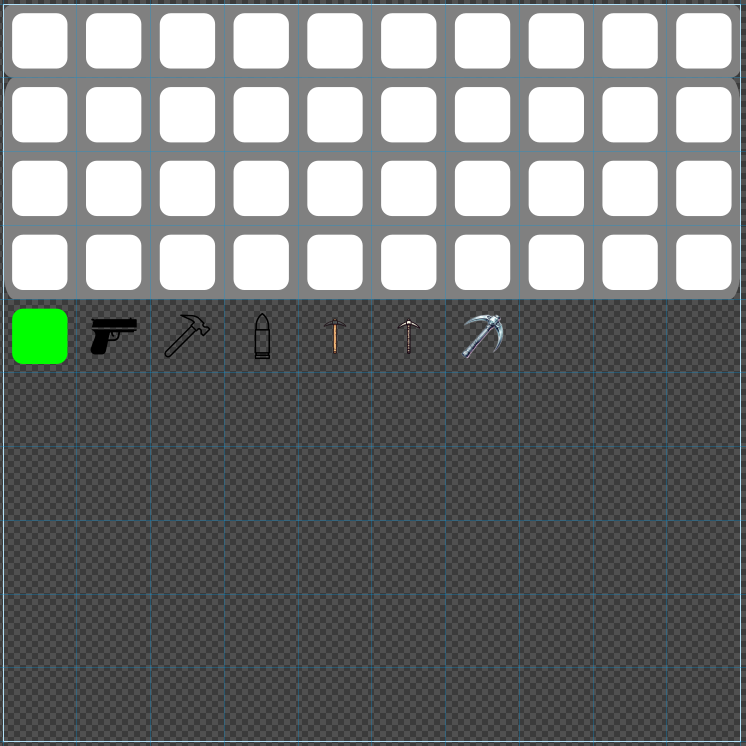
\includegraphics[width=0.8\textwidth]{chapters/system_architecture/sections/two_dimensional_graphics/resources/SpriteSheet.png}
        \caption{Inventory Sprite Sheet}
        \label{fig:inventory}
    \end{minipage}\hfill
    \begin{minipage}{0.45\textwidth}
    \begin{lstlisting}[language=json,firstline=1]
    {
        "width": 10,
        "height": 10,
        "items": [
            {
            "name": "hotbar",
            "x": 0,
            "y": 0,
            "width": 10,
            "height": 1
            },
        ]
    }
    \end{lstlisting}

    \caption{Inventory Sprite Sheet JSON}
    \label{lst:inventory_sprite_sheet_json}
    \end{minipage}
\end{figure}
\subsection{Heads Up Display} \label{sec:hud}
The HUD encapsulates all the 2d elements that are drawn on top of the 3d scene while the game is runnings.
This includes:
\begin{itemize}
    \item Crosshair
    \item FPS counter
    \item Player position
    \item Inventory
\end{itemize}

The Crosshair is a simple cross in the middle of the screen.
It is used to help the player aim.
It consists of 2 lines and does not use any textures.

The FPS counter is a simple text that shows the current frame rate.
It is drawn in the top right corner of the screen.
It uses the symbols texture.

The player position is a simple text that shows the current position of the player.
It is drawn in the top left corner of the screen.
It uses the symbols texture.

The inventory is a collection of images that represent the items the player has.
It is drawn at the bottom of the screen.
It uses both the items texture containing the HUD items and the texture containing the alphabet.
The images of the items are drawn first and then the text is drawn on top of them.
It is done in this order to optimize the performance by minimizing the number of times a texture is set to 2.

All the elements of the HUD have their own positions and sizes.
Each element is either placed in some position on the screen or is placed relative to some other element.
\subsection{Menu} \label{sec:menu}
Menu is a lot more complicated than the HUD which is described in \autoref{sec:hud}.
Because of that we decided to create a framework for creating menus.
This framework was heavily inspired by Flutter.
It uses the same concepts and terminology.
The overall idea is that everything is a widget.
A widget is a class that has a \texttt{Render} method as well as a \texttt{GetSize} method.
The \texttt{Render} method takes a context which includes information about the position and size on the screen that the widget can render to.
Some widgets also have children so the overall structure of the menu is a tree of widgets.

An example of a widget is shown in \autoref{fig:example_widget}.
This widget renders the main menu of the game.
The rendering logic of this widget can be seen in \autoref{fig:widget_logic}.
The idea is as follows.
The root widget calls the render method of it's child which is the \texttt{Background} widget.
The \texttt{Background} widget renders a background color.
Then the \texttt{Background} widget calls the render method of it's child which is the \texttt{Column} widget.
This widget renders it's children in a column but to do that it first needs to know the size of each of its children.
Based on that information it will call a render method of each child with the appropriate context.
Each child asks it's children for their size recursively until it reaches a leaf widget.
The process stops at the leaf and the render method is called on the children of the column widget.

This is a simplified version of the rendering logic as each widget has multiple options and rules that change how it or it's children are rendered.
For example, the \texttt{Column} widget has a \texttt{alignment} property which changes how the children are aligned.
The \texttt{Button} widget in the \autoref{fig:widget_logic} itself is a tree of widgets.

This approach of rendering the menu is very flexible and allows for a lot of customization.
It improves on the method used to render the HUD described in \autoref{sec:hud}.
This approach is not common in game development.
Usually menus are created by putting elements on the screen at specific positions. % TODO: cite something
In this part we believe that our approach is better than the traditional one and improves on approaches used in most popular game engines like Unity or Godot.

\begin{figure}[H]
    \centering
    \begin{minipage}{0.45\textwidth}
        \centering
        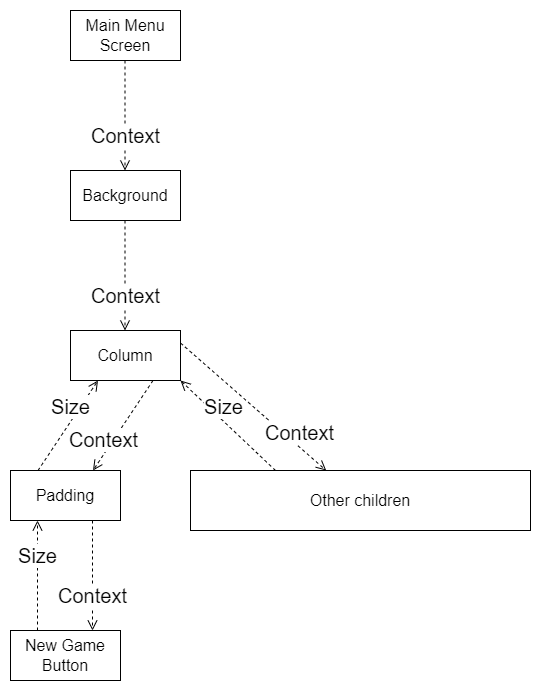
\includegraphics[width=0.8\textwidth]{chapters/system_architecture/sections/two_dimensional_graphics/resources/widget_logic.drawio.png}
        \caption{Widget rendering logic.}
        \label{fig:widget_logic}
    \end{minipage}\hfill
    \begin{minipage}{0.45\textwidth}
        \centering
        \includegraphics[width=0.8\textwidth]{chapters/system_architecture/sections/two_dimensional_graphics/resources/main-menu.png}
        \caption{Main menu.}
        \label{fig:example_widget}
    \end{minipage}
\end{figure}
\chapter{Main components}
\todo{write something about the components design overview or whatever}

\section{Animator}

The \texttt{Animator} class is responsible for animating the models loaded by \texttt{ModelLoader}.
It takes animation keyframes and interpolates them using Quaternion Slerp and Vector3 Lerp which are provided by AssimpNet.
It then uses the interpolated keyframes to calculate the transformation matrices for each bone in the model which are later passed to the shader.
\section{Model Loader}\label{model_loader}

The model loader is responsible for loading models from the file system.
It loads COLLADA files using AssipmNet to convert them to model class objects.
Each vertex in the mesh of the model must be dependent on at most 4 bones.
It creates VAOs for each mesh of the model, stores them in the Model class object, loads a PNG file, and stores it in a Texture class object.
\todo{I think we could write more about the modeling process itself (not necessarily here).
    Give some screenshots from Blender as well.
    It was a lot of work after all}

\section{Printer}

The \texttt{Printer} class is responsible for printing text on the screen.
It has a static constructor in which it creates a texture with the alphabet.
To achieve that it uses the SkiaSharp library.
After the texture is created \texttt{Printer} creates an array of Rectangles that describe the position of each letter on the texture.
These rectangles are passed to the shader when the text is printed.
This way only one texture is passed to the shader and the shader uses the rectangles to get the correct letter from the texture which improves performance.
The class also provides a method for printing a letter which is used in another method to print whole strings.
There are also methods for printing strings with the specified corner at the specified position.
\section{Sprite Renderer}\label{sprite_renderer}
\todo{this has to be rewritten because it says the same things as textures.tex}
The \texttt{SpriteRenderer} class is responsible for rendering 2D sprites.
It takes a PNG file and a JSON file as input and creates a texture and an array of rectangles that describe the position of each sprite on the texture.
It then uses the texture and the rectangles to render the sprites by passing the rectangle coordinates to the shader.
It only sets the texture once to boost performance.

An exemplary JSON file describing the position of the sprites on the texture is shown below:

\begin{verbatim}
    {
      "width": 10,
      "height": 10,
      "items": [
        {
          "name": "someItem",
          "x": 2,
          "y": 3,
          "width": 2,
          "height": 1
        },
        \dots
      ]
    }
\end{verbatim}


The width and height describe the size of the sprite sheet.
The \texttt{x,y} coordinates describe the position of the sprite on the sprite sheet.
The width and height describe the size of the sprite.
The name of the item is used to identify the sprite.

\todo{Screenshots? FPS, position, ...}
\section{Menu}
The \texttt{Menu} class is responsible for rendering the menu and handling user input.
It makes use of \texttt{SpriteRenderer} to render buttons and graphics.
It makes use of the \texttt{Printer} class to render text.
The menu is described in more detail in \autoref{subsec:menu}.

\section{Chunk Generator} \label{chunk_generator}
The Chunk Generator component is responsible for procedural terrain generation.
The generation process is encapsulated inside the \texttt{ChunkFactory} class.

A chunk is generated in two main steps:
\begin{enumerate}
    \item A scalar field of a given size is created.
          The values of the scalar field are generated based on the values of Perlin noise.
          This step is performed by the \texttt{ScalarFieldGenerator} class.
    \item The marching cubes algorithm is used to create a mesh;
          positions and normal vectors of the mesh's vertices are obtained in this step using the \texttt{MeshGenerator} class.
\end{enumerate}
\section{Chunk management system} \label{sec:chunk-worker}
The majority of the game logic is handled by a single thread.
The only two exceptions are the physics engine (external library) and the chunk management system.
The chunk management system is split between two threads: the main thread (the thread that the rest of the application is running on) and the \textit{chunk worker's} thread.
The worker's thread is concerned with operations that are either CPU-intensive or could take a long time to execute.
More specifically, the chunk worker is performing the following operations:
\begin{enumerate}
    \item loading saved chunks from disk and generating new chunks,
    \item saving chunks to disk,
    \item updating chunks.
\end{enumerate}
The system is built around the producer-consumer pattern, i.e. the main thread communicates with the worker's thread (and \textit{vice versa}) using queues.
It's important to note that depending on the stage of an operation either thread can be the \textit{producer} or the \textit{consumer}.
We will now describe the workflow for each of the operations mentioned before.

\subsection{Loading and generating chunks} \label{subsec:loading-and-generating}
On each render frame, the main thread calls the \texttt{UpdateCurrentPosition} method.
This method, based on the camera's current position and the render distance, determines which chunks should be loaded into the game.
If a chunk isn't already loaded or isn't queued for loading, the position of the chunk is enqueued into the \texttt{chunksToLoad} queue.

The worker thread in the \texttt{LoadChunks} function dequeues the positions of the chunks to be loaded from the disk.
If a chunk is not saved on the disk, it is generated.
The loaded/generated chunk is then enqueued into the \texttt{loaded} queue.

The main thread through the \texttt{ResolveLoaded} function dequeues a chunk and performs the following actions:
\begin{enumerate}
    \item creates a vertex array object for the chunk's mesh,
    \item creates a collision surface for the chunk,
    \item adds the chunk to the list of scene's chunks for rendering.
\end{enumerate}

It's worth noting that the operations in \texttt{ResolveLoaded} function have to be performed on the main thread because they interact with OpenGL and the physics engine APIs.
\subsection{Saving chunks}
Saving chunks is handled by a process similar to the one discussed in \autoref{subsec:loading-and-generating}.
On each frame, the main thread in the \texttt{DeleteChunks} function determines which chunks are too far from the player and thus should be removed from the game and saved to disk.
Positions of these chunks are enqueued into the \texttt{chunksToSave} queue, and their resources are freed.
More precisely, the removal takes place only if the number of chunks in the game exceeds a certain limit.
This is so that chunks are not deleted and loaded again constantly when the player moves back and forth between chunks.

The worker thread dequeues chunks' positions from the \texttt{chunksToSave} queue and saves the scalar field associated with a given chunk on the disk.
\subsection{Updating chunks}
Terrain modification consists of two main steps:
\begin{enumerate}
    \item the scalar field for the modified chunk has to be altered, which involves iterating over a 3-dimensional array of numbers and modifying the values stored in that array using some function,
    \item a new mesh has to be generated based on the new values of the scalar field.
\end{enumerate}
Since the modifications happen 60 times a second and the number of operations they require is rather big (of the order of the chunk size, i.e. $16^3$) it's unfeasible to do them on the main thread without severe lags.
Thus most of the work related to terrain modification is delegated to the worker thread.

The workflow for terrain modification can be described as follows.
The main thread in the \texttt{Pickaxe.ModifyTerrain} method determines which chunks are going to be affected by the terrain modification, and adds them to a buffer \texttt{buffer}.
Once all the chunks are in \texttt{buffer}, we set the \texttt{IsProcessingBatch} flag to \texttt{true} (while set to true, no further terrain modifications will be registered) and enqueue each of them into the \texttt{modificationsToPerform} queue along with some additional information (passed in the form of an instance of \texttt{ModificationArgs} struct) necessary to perform the modification.
A very important piece of information is the \texttt{batchSize} which is the size of \texttt{buffer} (its importance will become apparent later).

The worker thread dequeues chunks from the \texttt{modificationsToPerform} queue.
It modifies the scalar field using the information passed in \texttt{ModificationArgs} and generates a new mesh based on the scalar field.
Once new vertices for the mesh are calculated, it enqueues the chunk together with \texttt{batchSize} (retrieved from \texttt{modificationArgs}) into the \texttt{updatedChunks} queue.

In the \texttt{ResolveUpdated} function the main thread dequeues the \texttt{(chunk, batchSize)} pair from the \texttt{updatedChunks} queue and adds \texttt{chunk} to the \texttt{currentBatch} list.
Once the number of chunks in \texttt{currentBatch} is equal to \texttt{batchSize} of the dequeued chunk, it means that the main thread has "received back" all of the chunks from a single modification call.
The main thread then updates the GPU buffers with the new vertices of the chunk's mesh and updates the shape of the collision surface in the physics engine for each chunk from \texttt{currentBatch}.
Once the whole \texttt{currentBatch} is updated, the \texttt{IsProcessingBatch} flag is set back to false.

The whole process is depicted in \autoref{fig:chunk-worker}.
\begin{figure}[h] % https://drive.google.com/file/d/1TzJouYAys_fz1GkhppZsqoh9yFn62twL/view?usp=sharing
    \centering
    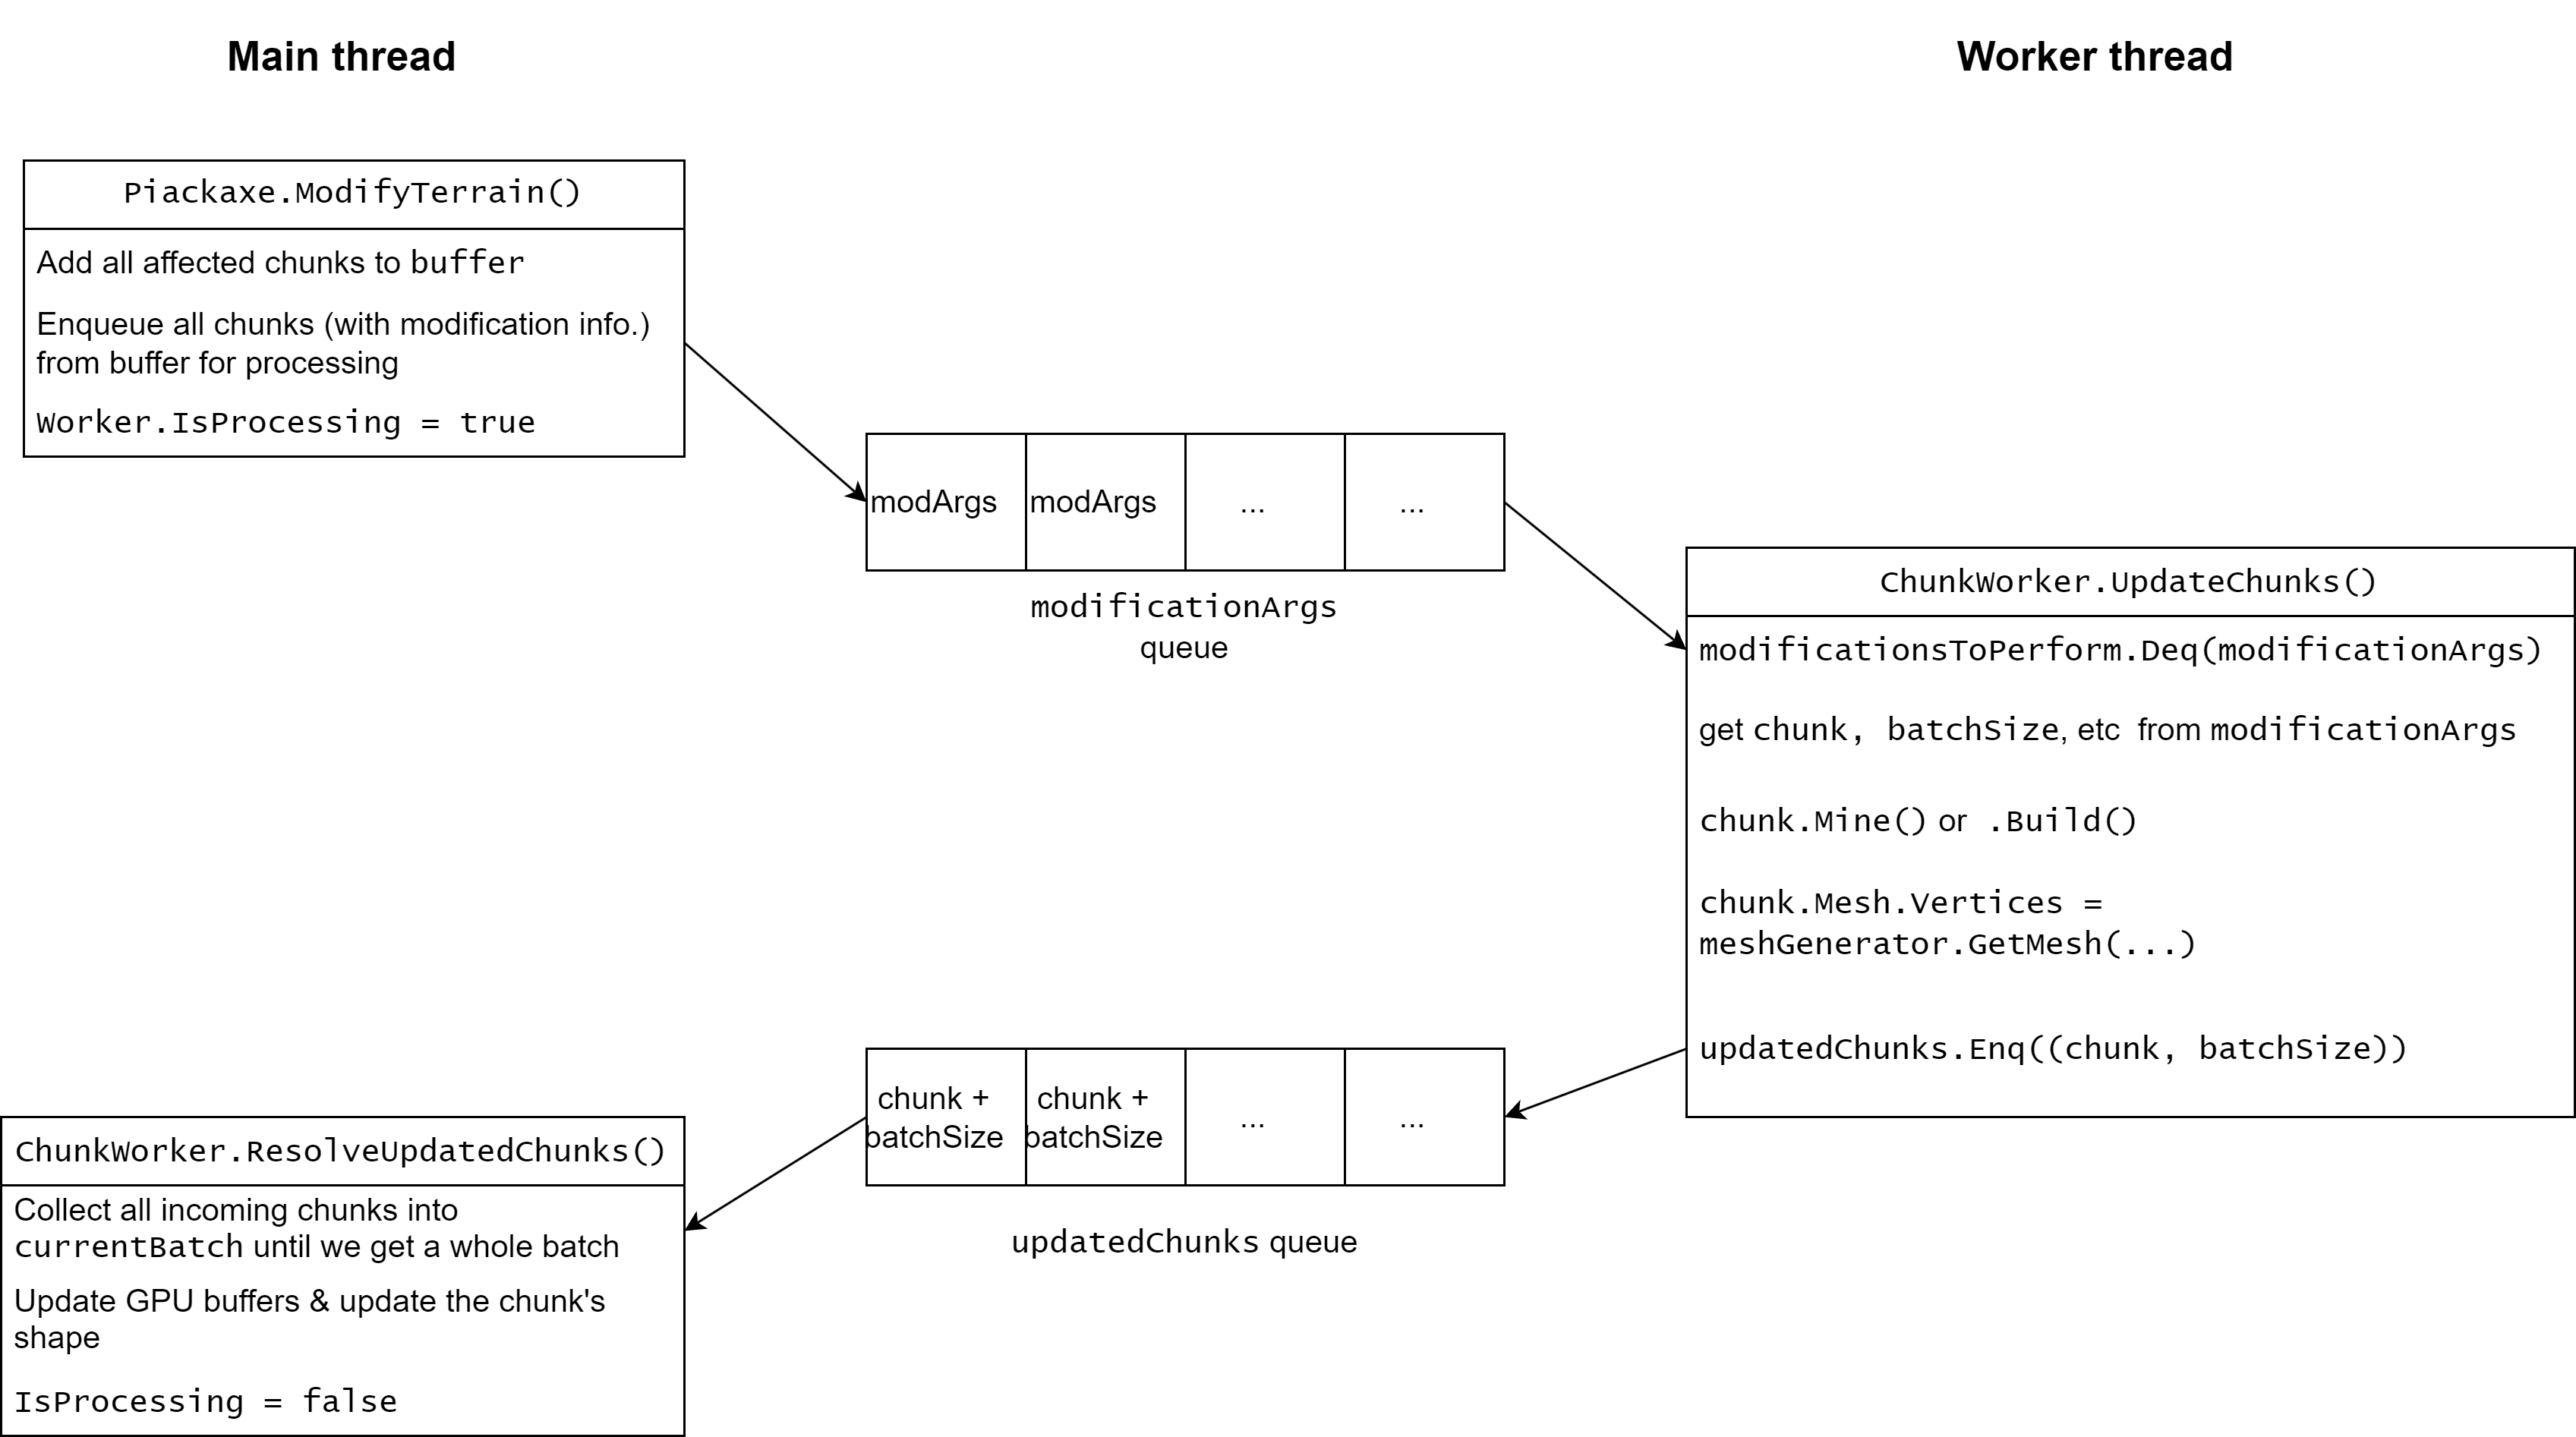
\includegraphics[width=1\textwidth]{chapters/main_components/sections/chunk_worker/resources/chunkWorker.drawio.png}
    \caption{Terrain modification in the chunk management system}
    \label{fig:chunk-worker}
\end{figure}

The reason for processing chunks in batches rather than individually is simple.
If we modify chunks one by one it may be the case that when the terrain is rendered, one chunk has already been modified, while its neighbor has not, resulting in a visible gap between the two.
This problem can be seen in \autoref{fig:gaps-between-chunks-chunk-worker} which comes from an early stage of the game's development.
\begin{figure}[h]
    \centering
    \includegraphics[width=0.8\textwidth]{chapters/main_components/sections/chunk_worker/resources/gaps-between-chunks.png}
    \caption{Gaps between chunks appearing during terrain modification}
    \label{fig:gaps-between-chunks-chunk-worker}
\end{figure}

One drawback of this approach is that the main thread doesn't register new chunks for modification while the whole previously enqueued batch hasn't been processed.
This could cause the modification rate to be irregular should the main thread "drop" a lot of modifications.
To deal with this problem, the modification depends on the time elapsed between two modifications.

\section{Physics}
The Physics component is responsible for collision detection, ray casting, and physical modeling.
The main purpose of this component is to expose the various functionalities of the BepuPhysics2 library to the rest of the system.
The component also makes extensive use of the code from the BepuPhysics2 Demos project.

Each game object is represented by a \textit{body} (each body has an associated \textit{body handle}) in the physics engine.
This one-to-one mapping is stored in the \texttt{Scene} class in an object of \texttt{SimulationMembers} type.
\texttt{SimulationMembers} allows for adding and removing simulation members as well as accessing handles to bodies in the physics engine associated with a given game object.
Game objects are represented by either simple or composite shapes in the physical simulation.
Simple shapes used in the game include cylinders, capsules, and boxes.
Composite shapes arise by composing simple shapes.
\question{Should the car be described in more detail (how to specify the axis of rotation for the wheels, etc.)}

To facilitate debugging, the Physics component also provides a way to extract all shapes from the simulation (and decompose composite shapes) which then can be shown in debug mode, see \autoref{fig:bounding-shapes}.
When shown, the bounding shapes can be either green or red depending on whether the corresponding bodies are in the active or inactive state in the physics engine.
In \autoref{fig:bounding-shapes} it can be seen that the player has been hit by a projectile which caused the player's body to become active (or \textit{awakend} using the BepuPhysics parlance) as indicated by the green bounding shape.
The projectile that hit the player can also be seen to be active.
On the other hand, the projectiles that fell to the ground and had been still for some time became inactive as marked by the red bounding shapes.
\begin{figure}[h]
    \centering
    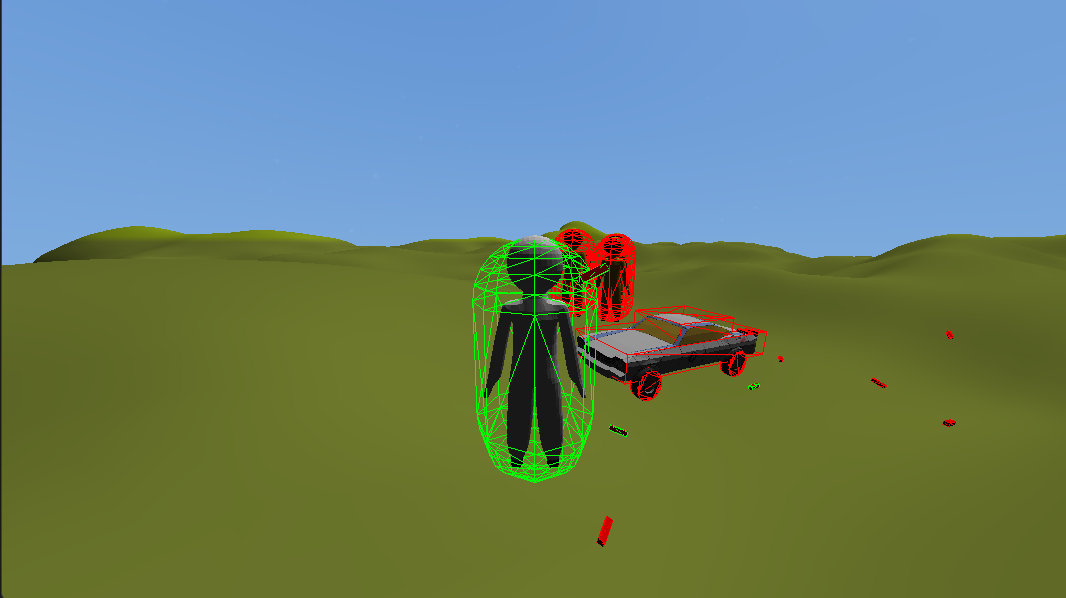
\includegraphics[width=0.8\textwidth]{chapters/main_components/sections/physics/resources/bounding-shapes.png}
    \caption{Game objects enclosed in bounding shapes for collision detection}
    \label{fig:bounding-shapes}
\end{figure}

The body that represents the terrain was created as a separate shape from the terrain mesh triangle-by-triangle.

Game objects can listen and respond to collisions by registering their contact callbacks via the API in \texttt{SimulationManager}.
Such objects implement the \texttt{IContactEventListener} interface whose implementations define the contact callbacks.
The only information about the collision is which two bodies collided and where.

Some game objects can cast rays.
An example of such an object is the player who uses a ray to define a place where terrain modification should take place.
Each ray in the physics engine has an ID number, direction, etc.
An object that wishes to cast rays has to therefore implement an interface (\texttt{IRayCaster}) that exposes all the necessary information.


\section{Scene}

The \texttt{Scene} class is responsible for storing all the objects in the game the player can interact with.
It is also responsible for disposing of them.
Here is the full list of objects stored in a \texttt{Scene} instance:

\begin{itemize}
  \item Chunks
  \item LightSources
  \item Projectiles
  \item Bots
  \item Cars
  \item Player
  \item Camera
  \item SimulationMembers
  \item SimulationManager
\end{itemize}


\section{Controllers}

There are eight controller classes in the project:

\begin{itemize}
  \item  \texttt{PlayerController}
  \item \texttt{BotsController}
  \item \texttt{ChunksController}
  \item \texttt{ProjectilesController}
  \item \texttt{VehiclesController}
  \item \texttt{LightSourcesController}
  \item \texttt{HudController}
  \item \texttt{BoundingShapesController}
\end{itemize}

All the controller classes serve the same purpose.
They exist to render objects and deal with object callbacks.
For example, \texttt{ProjectilesController} renders all existing projectiles and also removes the dead projectiles from the scene.
Each projectile has a \texttt{IsAlive} property which is read every time a render frame callback is called by the controller to check if the projectile is still alive.

\section{Context}

The Context component is responsible for input handling and performing actions on each frame.
There are two sources of user input considered in the video game: keyboard and mouse.
Keys and mouse buttons can be in one of three states: \textit{pressed}, \textit{down}, and \textit{up}.
Additionally, the mouse can also generate events when it's moved.

The \texttt{Context} class stores mappings between different types of input and actions that should be triggered by the given input.
Changes in the input state are tracked by OpenTK and the \texttt{Context} activates relevant actions as a response.
It is a convention that every class that registers new actions in the \texttt{Context} implements the \texttt{IInputSubscriber} interface.
Also, it is worth noting that, for better performance, the Context will only trigger actions associated with the input that has itself been previously registered.
\section{Transporter}
The Transporter component is vital for the spherical geometry mode of the game.
It is responsible for transporting game objects between spheres.
All transporters implement the \texttt{ITransporter} interface.

Each game object has a property \texttt{CurrentSphereId} that attains one of two values: 0 or 1 depending on which sphere the object is currently in (this property is a part of \texttt{ISimulationMember} interface).
Whenever an object moves, the Transporter determines whether it should be transported to the opposing sphere by calculating the object's distance from its current sphere's center.

The transportation process changes the object's position and velocity.
In the case of objects modeled as compound bodies, it is necessary to alter the positions and velocities of each of the components.
When a camera is attached to an object that gets transported, it also has to be updated accordingly.
More specifically, the Transporter transforms the camera's front vector and updates the information about the camera's current sphere.

The functionalities mentioned above are only relevant in the spherical geometry mode.
To make the system design consistent across all modes, there is also a \texttt{NullTransporter} implementation of the \texttt{ITransporter} interface which is used in hyperbolic and Euclidean geometry modes.
This is a dummy class with methods that don't do anything.
\chapter{User Manual}\label{ch:user_manual}
This section describes how to launch and later use the application.
The user controls were made with industry standards in mind, so the user should not have any problems with using them.
However, if the user does not have much experience with video games, this section will help them get started as it provides a detailed start-to-finish description of how to play the game.

\section{Launching the game}
The application starts in the main menu shown in \autoref{fig:main_menu}.
From here a new game can be started, a previous save can be loaded, or a save can be deleted.
The user can also view controls, and exit the game.
To start a game for the first time, the user has to click on the "New Game" button which will show the "New Game Screen".

When the game is running the user can press the \keys{\escwin} key to show the main menu or hide it.
While the game is running the main menu will also show a "Resume" button which will resume the game and hide the menu.

\begin{figure}[H]
    \centering
    \includegraphics[width=0.8\textwidth]{chapters/user_manual/resources/main-menu.png}
    \caption{Main menu}
    \label{fig:main_menu}
\end{figure}
\section{New Game Screen}
The game can be started from the New Game screen shown in \autoref{fig:new_game}.
To start a game, the user has to click on the "Input Game Name" input text box.
This will allow them to enter a name for the game.
If there is no game save with the same name, the text box will light up green.
If there is already a game save with the same name, the text box will light up red.
If the box is green, the user can press one of the buttons to start a new game in the chosen geometry.

\begin{figure}[!htb]
    \centering
    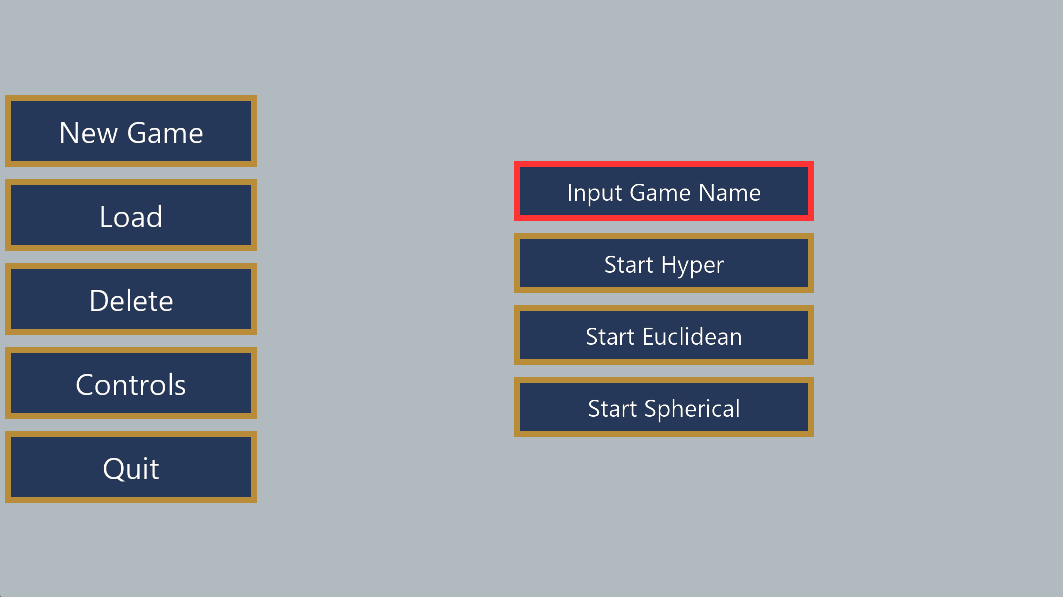
\includegraphics[width=0.8\textwidth]{chapters/user_manual/resources/new-game-no-input.png}
    \caption{New Game screen}
    \label{fig:new_game}
\end{figure}
\section{Load Game Screen}
The game can be loaded from the Load Game screen shown in \autoref{fig:load_game}.
This screen displays your 9 most recent saves.
The user can load a save by clicking a tile corresponding to the save.
To load a more recent save the user has to first delete more recent saves using the "Delete Game" described in \autoref{delete_save_screen}

\begin{figure}[h]
    \centering
    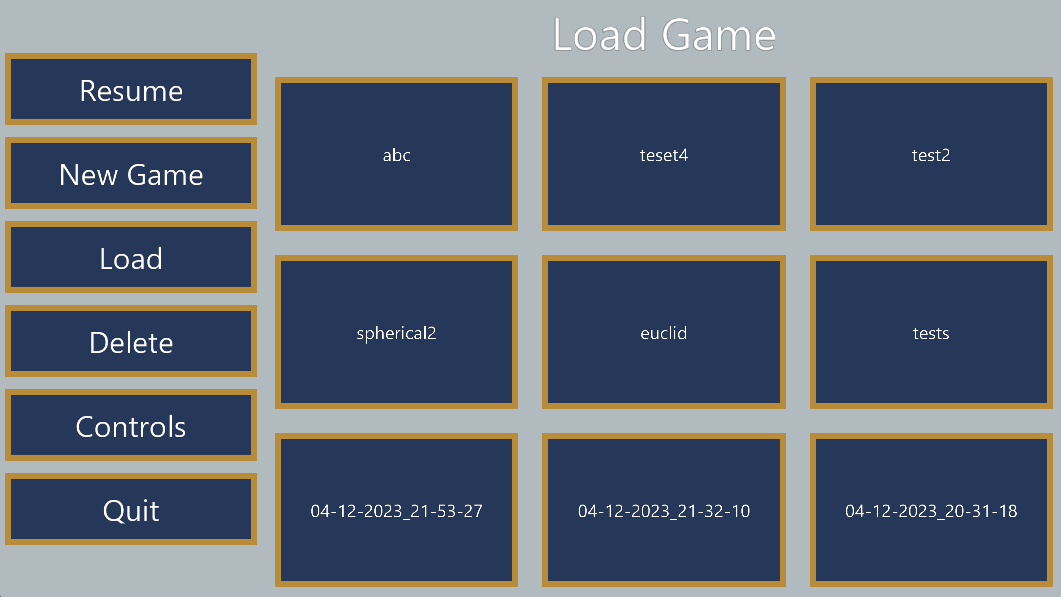
\includegraphics[width=0.8\textwidth]{chapters/user_manual/resources/load-game.png}
    \caption{Load Game screen}
    \label{fig:load_game}
\end{figure}
\subsubsection{Delete Save Screen} \label{delete_save_screen}
The "Delete Game" screen shown in \autoref{fig:delete_save} allows you to delete your saves.
It will display your 9 most recent saves.
To delete a save click on its name.
If a game is currently running you cannot delete its save.

\begin{figure}[H]
    \centering
    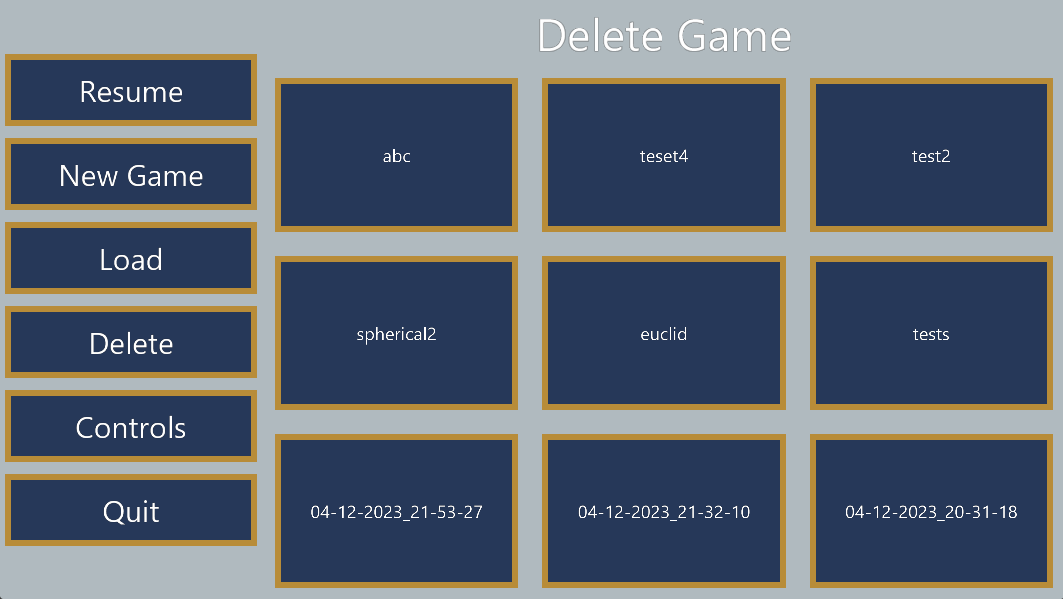
\includegraphics[width=0.8\textwidth]{chapters/user_manual/resources/delete-game.png}
    \caption{Delete Save screen}
    \label{fig:delete_save}
\end{figure}
\section{Controls}
The controls for the game are presented in \autoref{tab:game_key_functions}.
If the user forgets them, they can press the "Controls" button in the menu at any time to see them in the game, as shown in Figure \ref{fig:controls}.

\begin{table}[h]
    \centering
    \begin{tabular}{|m{3cm}|m{8cm}|}
        \hline
        \textbf{Key}              & \textbf{Function}                                              \\
        \hline
        \keys{W}                  & Move forward.                                                  \\
        \hline
        \keys{S}                  & Move back.                                                     \\
        \hline
        \keys{A}                  & Move left.                                                     \\
        \hline
        \keys{D}                  & Move right.                                                    \\
        \hline
        \keys{\shift}             & Sprint.                                                        \\
        \hline
        \keys{\SPACE}             & Jump.                                                          \\
        \hline
        \texttt{Left Mouse}       & Use item.                                                      \\
        \hline
        \texttt{Right Mouse}      & Use item's second ability.                                     \\
        \hline
        \keys{\escwin}            & Show/Hide menu.                                                \\
        \hline
        \keys{\tab}               & Switch camera between 1st and 3rd person.                      \\
        \hline
        \texttt{Scroll}           & Change curvature (works only in hyperbolic geometry).          \\
        \hline
        \keys{0} through \keys{9} & Select item.                                                   \\
        \hline
        \keys{C}                  & Enter car.                                                     \\
        \hline
        \keys{F}                  & Flip car (works only outside the car).                         \\
        \hline
        \keys{L}                  & Leave car.                                                     \\
        \hline
        \keys{Y}                  & Toggle flashlight/Toggle car reflectors (when inside the car). \\
        \hline
        \keys{F1}                 & Toggle cinematic mode.                                         \\
        \hline
        \keys{F3}                  & Toggle showing hitboxes.                                       \\
        \hline
    \end{tabular}
    \caption{Keyboard Key Functions for Game Controls}
    \label{tab:game_key_functions}
\end{table}

\begin{figure}[H]
    \centering
    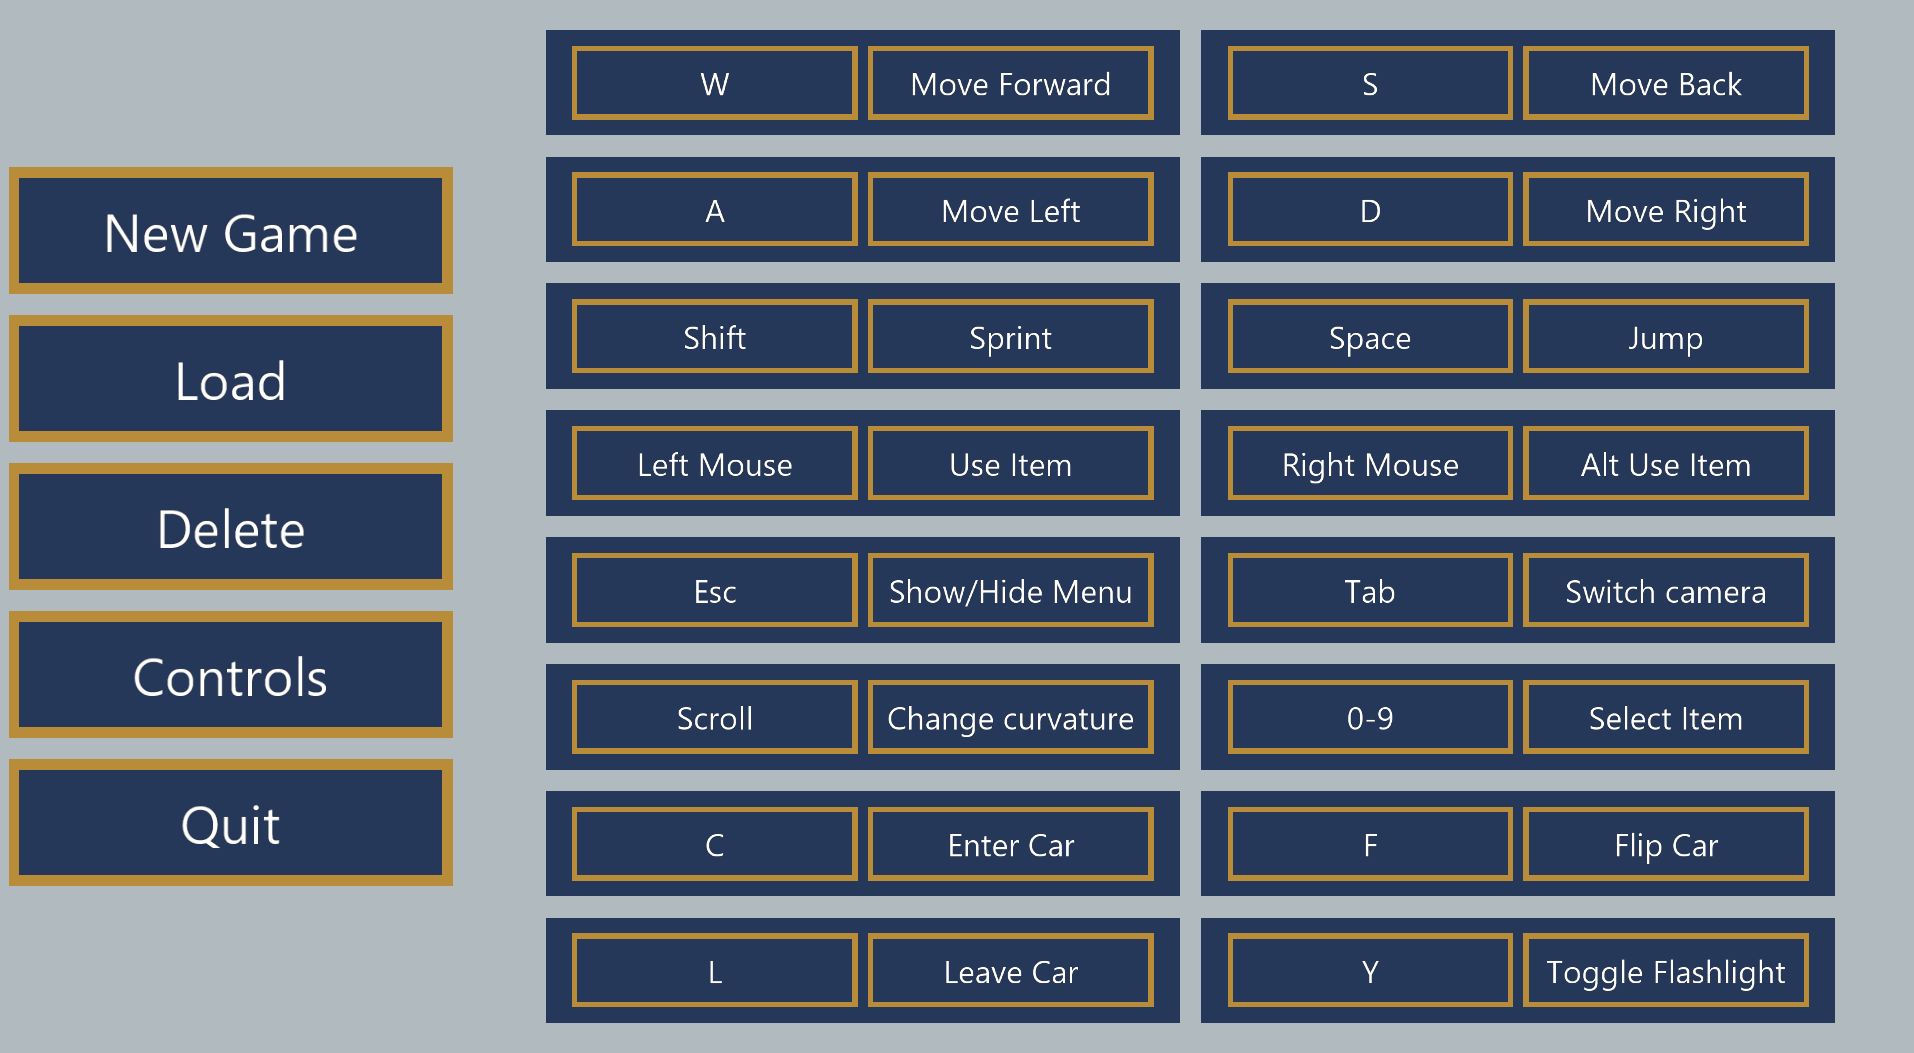
\includegraphics[width=0.8\textwidth]{chapters/user_manual/resources/controls.png}
    \caption{Controls screen}
    \label{fig:controls}
\end{figure}
\section{Items}
Items are a big part of the game.
Different items in the game have different uses.
Description of all the in-game items can be found in \autoref{tab:mytable}.
To use the items the player has to first select the desired item using number keys \keys{0} through \keys{9}.
The selected item will be highlighted in the inventory as shown in \autoref{fig:inventory}, in which the selected item is the gun.
The player can use the item by pressing the left mouse button (\texttt{LMB}) or the right mouse button (\texttt{RMB}).
The effect of the item depends on the item itself and the mouse button used.

\begin{table}[h]
    \centering
    \begin{tabular}{|c|p{5cm}|p{5cm}|}
        \hline
        Item                                                                         & \texttt{LMB} Effect                                                                   & \texttt{RMB} Effect \\
        \hline
        
\includegraphics[width=1cm]{chapters/user_manual/resources/bullet.png}       & No effect                                                                             & No effect           \\
        \hline
        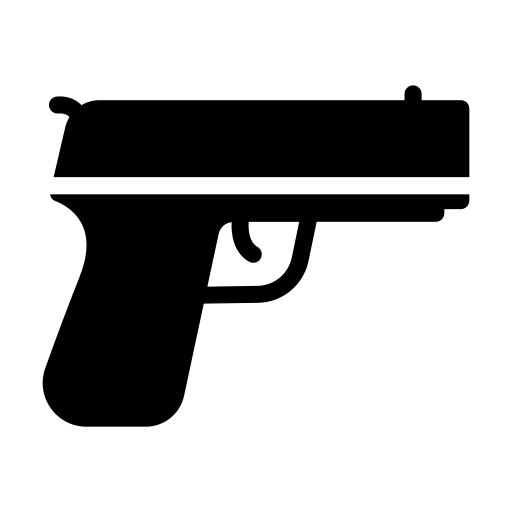
\includegraphics[width=1cm]{chapters/user_manual/resources/pistol.png}       & Fires a bullet if there is one in the inventory. Removes a bullet from the inventory. & No effect           \\
        \hline
        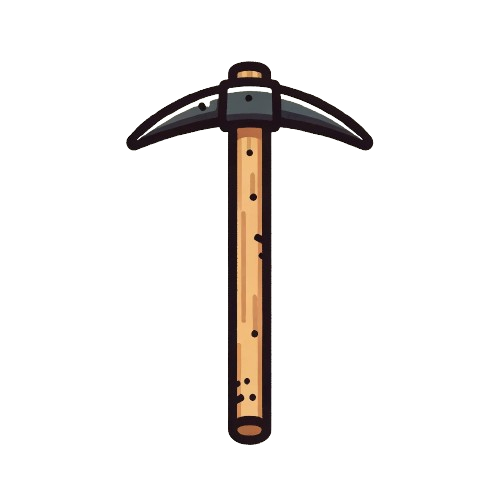
\includegraphics[width=1cm]{chapters/user_manual/resources/pickaxe-slow.png} & Mines slowly.                                                                         & Builds slowly.      \\
        \hline
        
\includegraphics[width=1cm]{chapters/user_manual/resources/pickaxe-mid.png}  & Mines.                                                                                & Builds.             \\
        \hline
        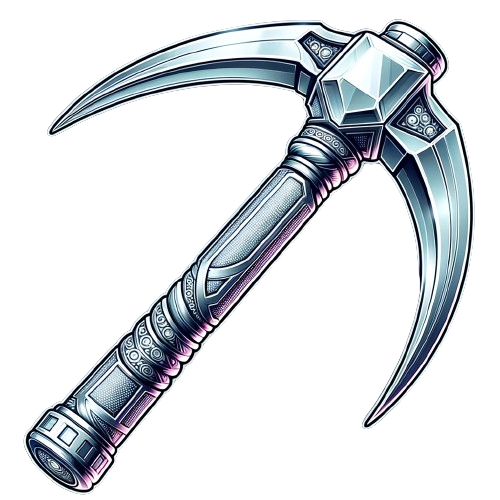
\includegraphics[width=1cm]{chapters/user_manual/resources/pickaxe-fast.png} & Mines quickly.                                                                        & Builds quickly.     \\
        \hline
    \end{tabular}
    \caption{Table of in game items}
    \label{tab:mytable}
\end{table}

\begin{figure}[H]
    \centering
    
\includegraphics[width=0.8\textwidth]{chapters/user_manual/resources/inventory.png}
    \caption{Inventory}
    \label{fig:inventory}
\end{figure}
\section{Gameplay}\label{sec:gameplay}
After the game is started, the user can finally start playing.
At the start, the screen will look like in \autoref{fig:gameplay}.
The user can see their position in the top left corner, the current frames per second in the top right corner, and the inventory in the bottom of the screen.
In the middle of the screen, there is a crosshair that shows where the user is aiming.
The user can also see their character model.
By using the controls described in \autoref{sec:controls}, the user can start moving around and exploring the world.


\begin{figure}[h]
    \centering
    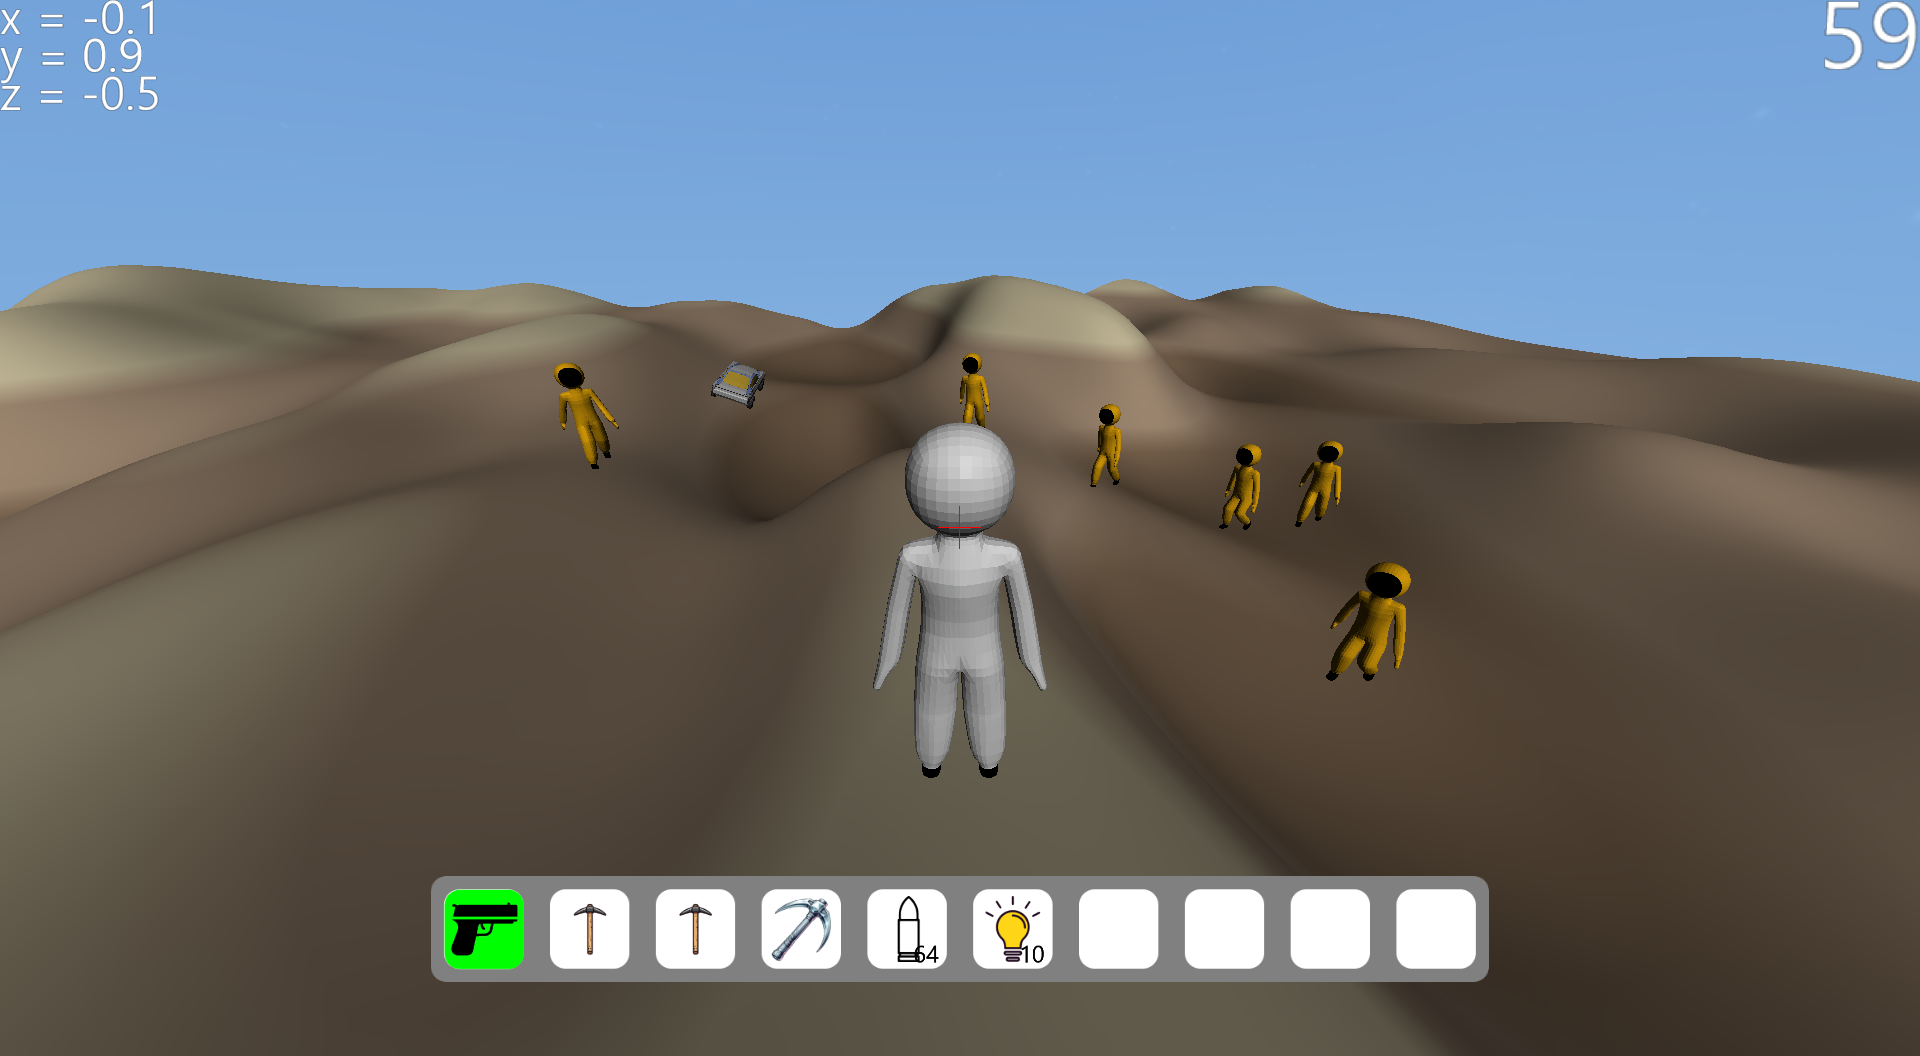
\includegraphics[width=0.8\textwidth]{chapters/user_manual/resources/gameplay.png}
    \caption{Controls screen}
    \label{fig:gameplay}
\end{figure}
\chapter{Functionalities}
\todo{This chapter should have a different folder name and the tex file should also be renamed.
    Maybe we could split the thesis into chapters like Theoretical foundations, System architecture, Functionalities/Features/??? (move the terrain stuff here as well), ...}
\section{Environment}
Even though the game can be played in non-Euclidean spaces which makes it inherently unrealistic, we decided to add some elements that would make the scenes portrayed in the game feel familiar.
One such element is the Earth-like terrain, described in detail in the previous sections.
Another property of the real world that we wanted to capture in the game was the daytime cycle.
In the game, the full cycle is 10 minutes long, with 5 minutes long daytime and 5 minutes long nighttime.
We also added transitions between day and night to give the Earth-like experience of sunrise and sunset.
The scene during various times of the day is shown in \autoref{fig:cycle}.

\begin{figure*}[h]
    \centering
    \begin{subfigure}[b]{0.475\textwidth}
        \centering
        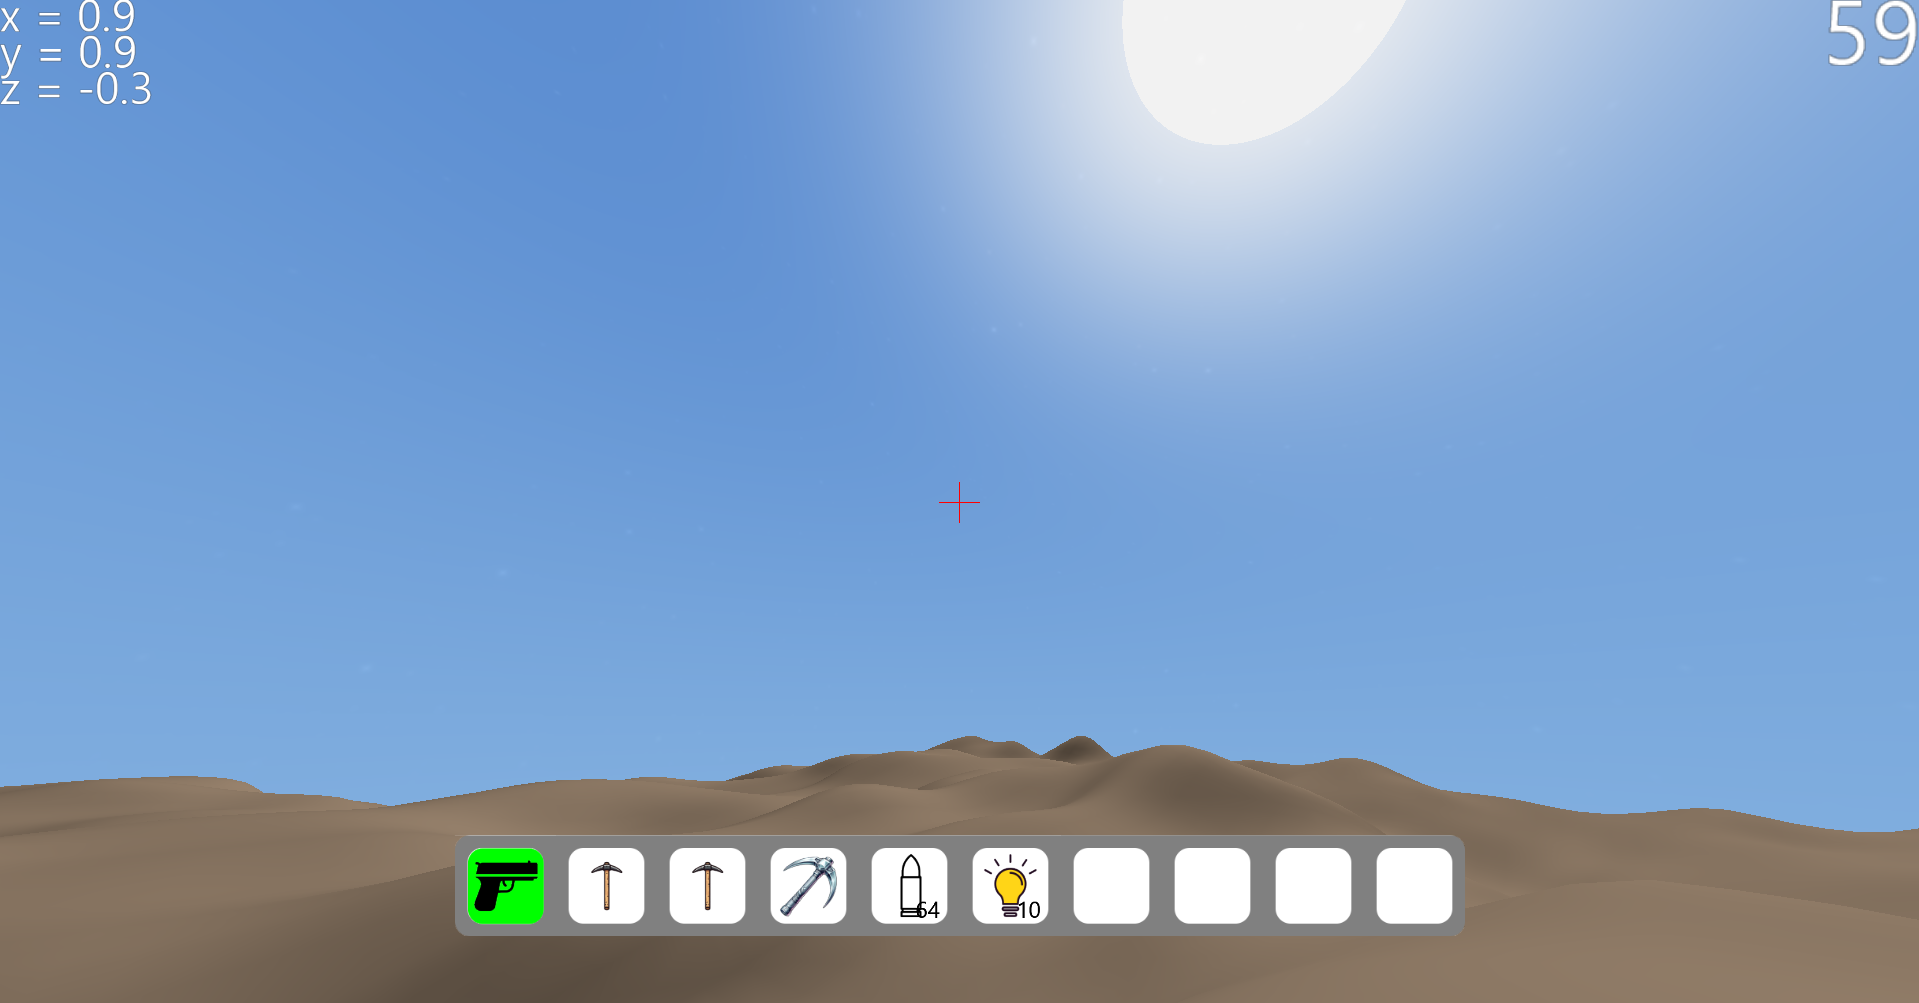
\includegraphics[width=\textwidth]{chapters/lighting/sections/environment/resources/day.png}
        \caption[]%
        {{\small Day}}
        \label{fig:cycle-day}
    \end{subfigure}
    \hfill
    \begin{subfigure}[b]{0.475\textwidth}
        \centering
        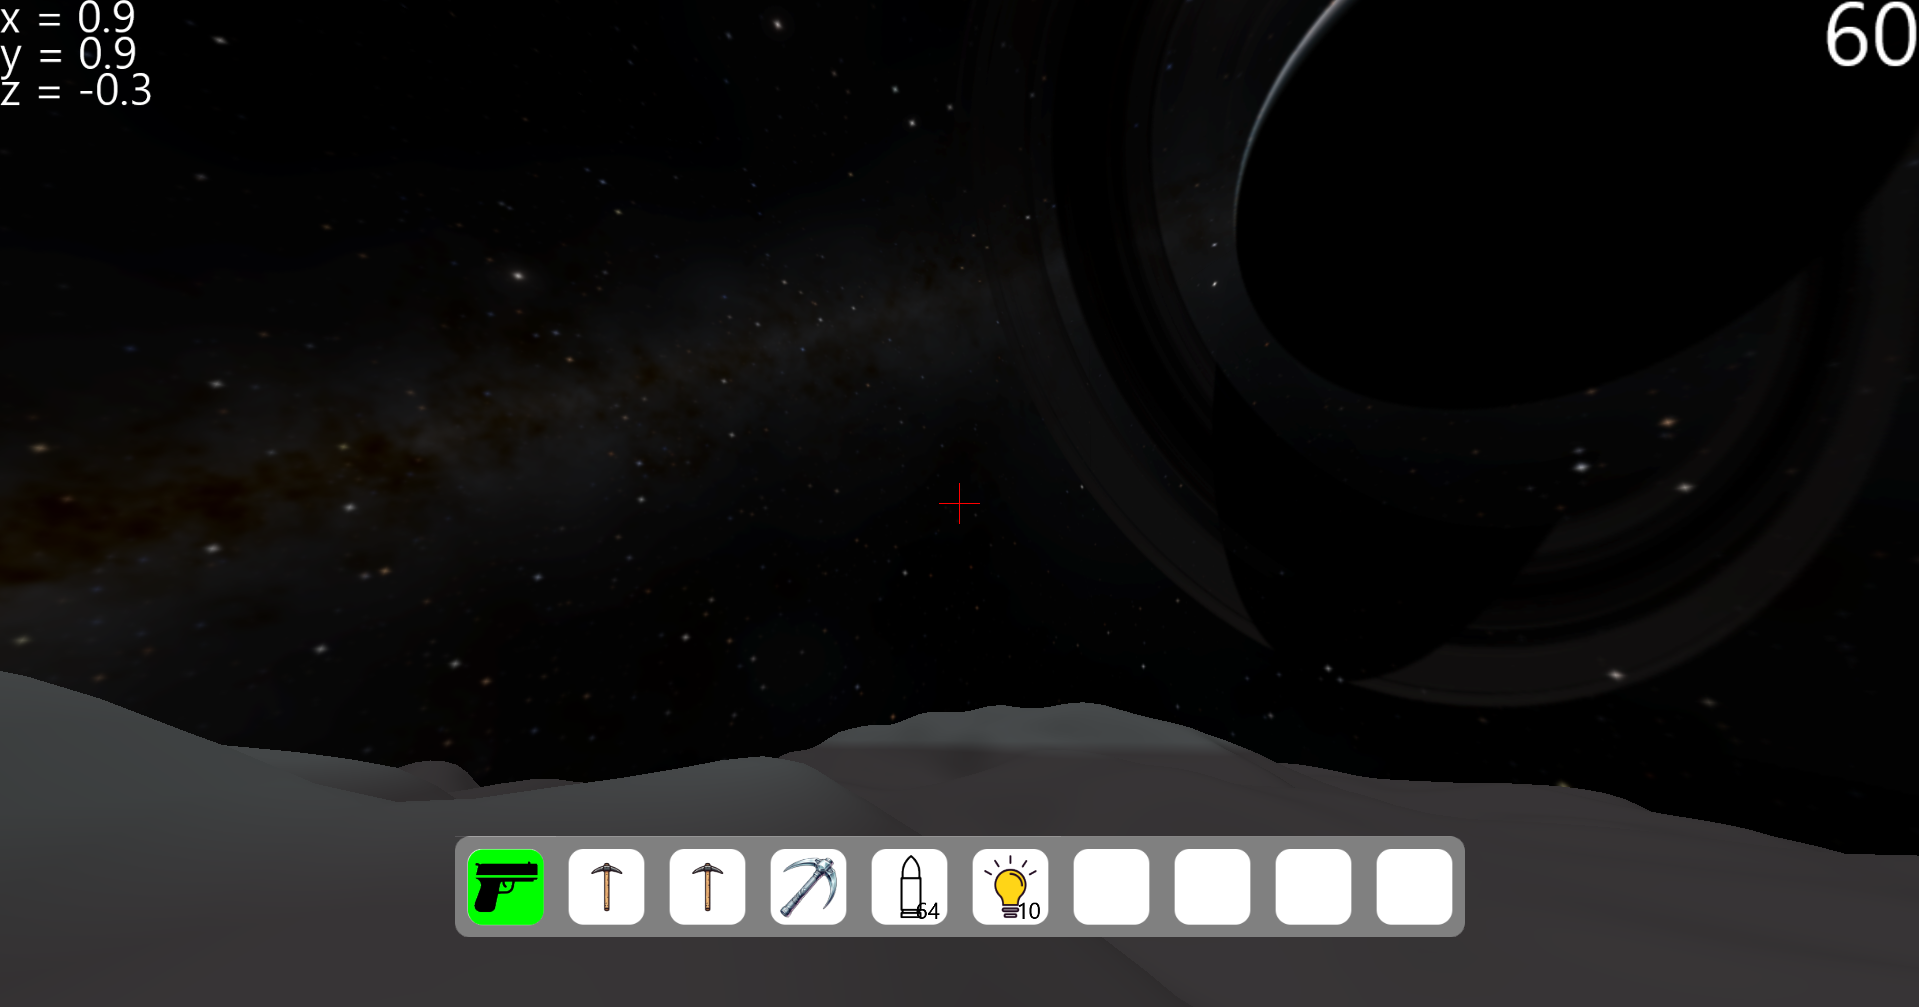
\includegraphics[width=\textwidth]{chapters/lighting/sections/environment/resources/night.png}
        \caption[]%
        {{\small Night}}
        \label{fig:cycle-night}
    \end{subfigure}
    \vskip\baselineskip
    \begin{subfigure}[b]{0.475\textwidth}
        \centering
        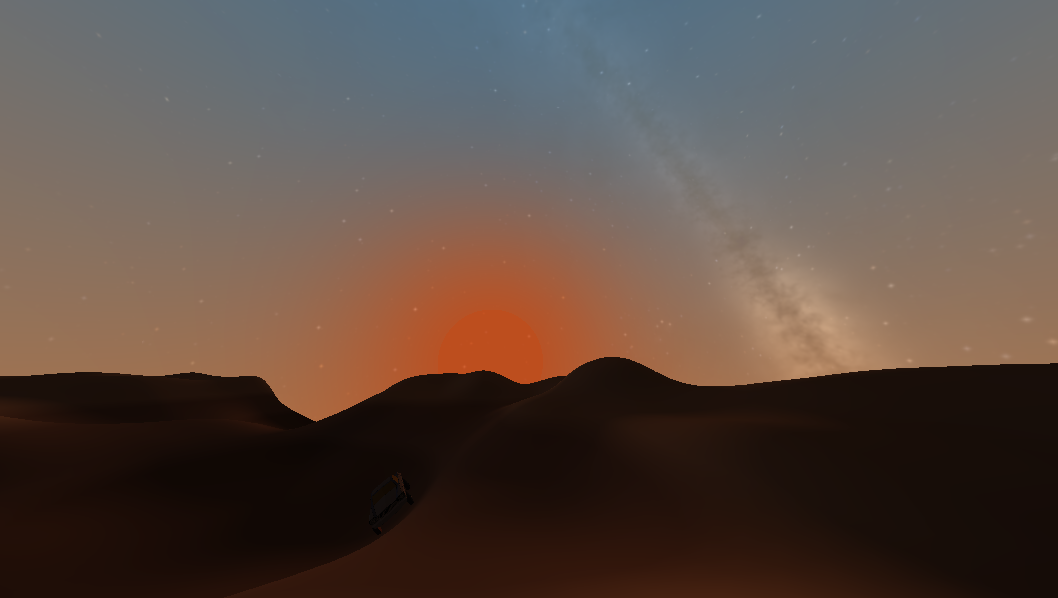
\includegraphics[width=\textwidth]{chapters/lighting/sections/environment/resources/sunrise.png}
        \caption[]%
        {{\small Sunrise}}
        \label{fig:cycle-sunrise}
    \end{subfigure}
    \hfill
    \begin{subfigure}[b]{0.475\textwidth}
        \centering
        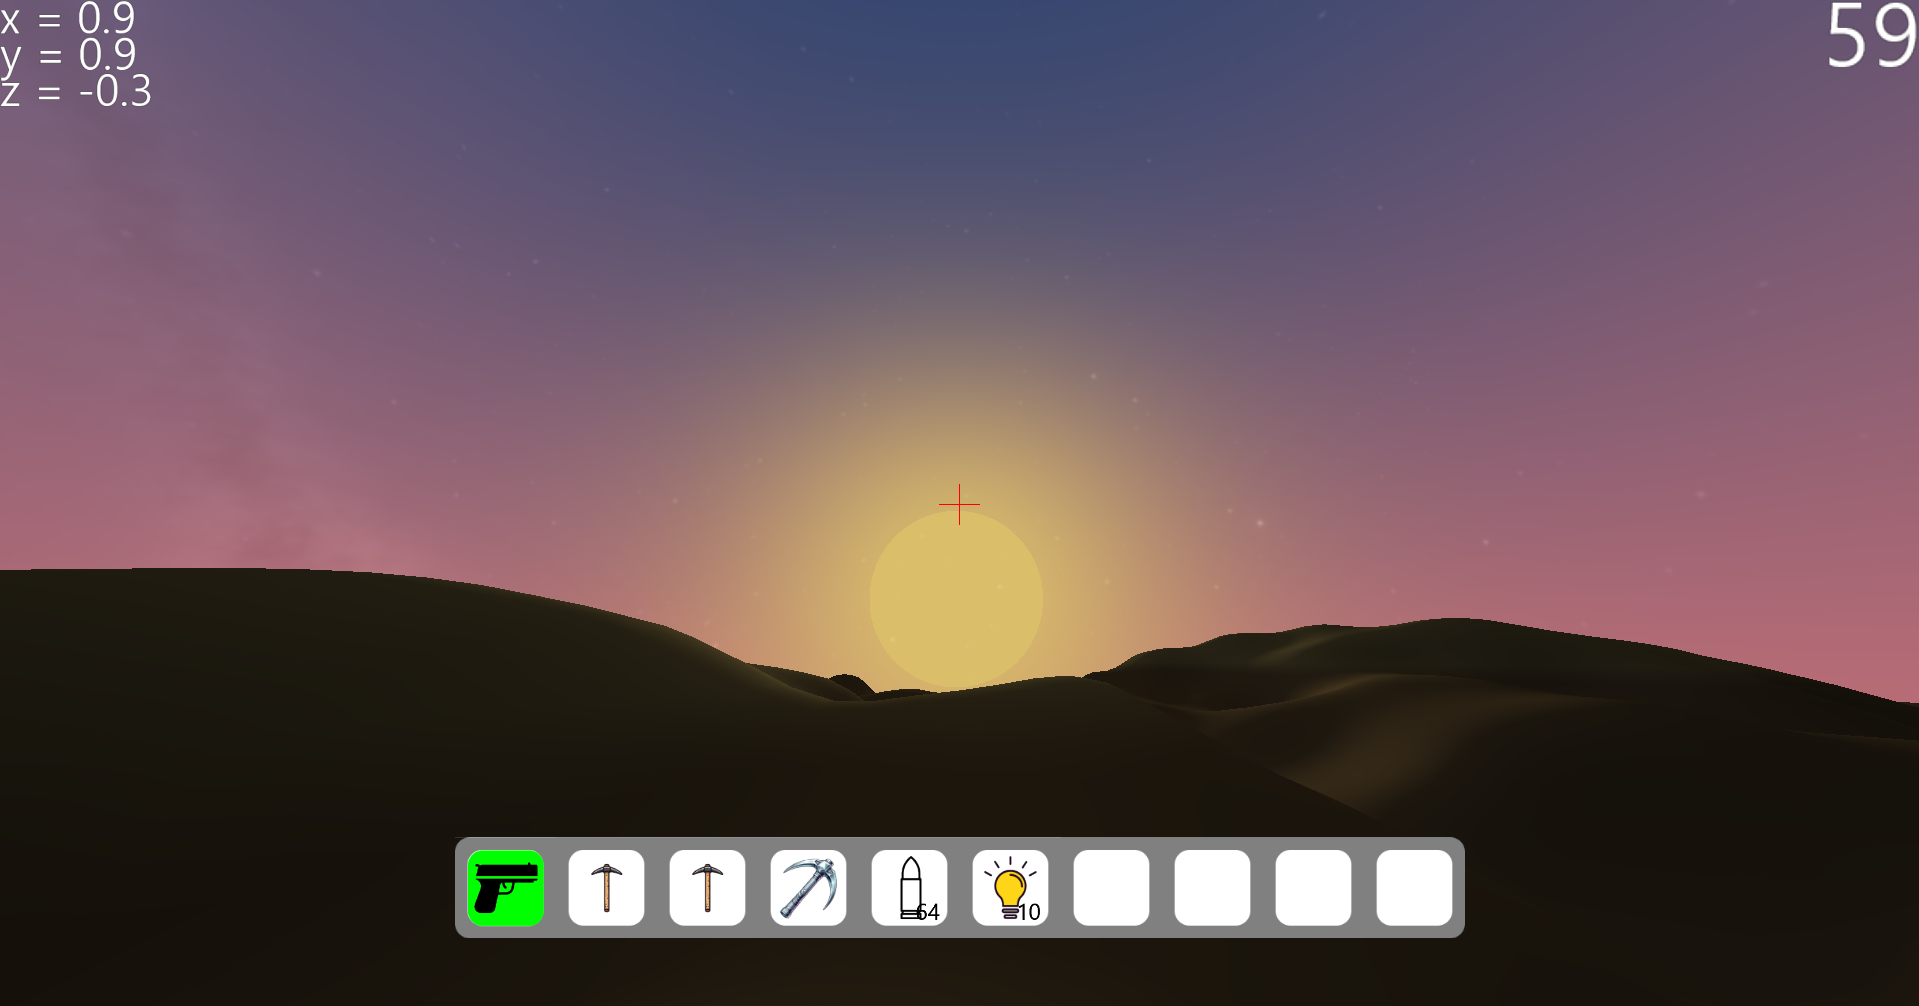
\includegraphics[width=\textwidth]{chapters/lighting/sections/environment/resources/sunset.png}
        \caption[]%
        {{\small Sunset}}
        \label{fig:cycle-sunset}
    \end{subfigure}
    \caption[]
    {\small Day night cycle in the game}
    \label{fig:cycle}
\end{figure*}

The implementation of the day-night cycle relies on two components: directional lighting (described in \autoref{subsec:directional-lighting}) which corresponds to the light coming from the sun and a \textit{skybox} representing the sky.
Conceptually, a skybox is a cube made out of 6 images, one per each side, that encompasses the scene thus creating an illusion that the world is much bigger than it is in reality.
A skybox can be implemented in OpenGL using a special type of texture, a \textit{cubemap}, i.e. a texture that contains 6 individual 2D textures.
In the game, we're using images of the night sky obtained from an HDR file \url{https://www.reddit.com/r/blender/comments/3ebzwz/free_space_hdrs_1/} using an online utility program \url{https://matheowis.github.io/HDRI-to-CubeMap/}.
The images were then slightly edited to make the stars appear larger.
The vertices of the cube passed to the vertex shader are transformed using the model, view, and projection matrices.
The model matrix is responsible for rotating the skybox (similarily to how stars appear to move across the night sky as the Earth is rotating).
The view matrix has to be modified so that the skybox doesn't move along with the camera.
The part responsible for translation can be removed from the view matrix by replacing the last row the the view matrix with the vector $[0, 0, 0, 1]$ \cite{LearnOpenGL-Cubemaps}.

The day is split into \textit{phases}, each characterized by the color of the sky at the zenith, the sky's color at the horizon, the color of the sun, and \textit{stars' visibility factor}.
In the fragment shader, we determine the color of each fragment.
This is done by first obtaining the zenith and horizon colors by interpolating between the corresponding colors for the previous and next phase based on the current time.
In the same manner, we obtain the current stars' visibility factor.
Then, we obtain a sky color for a given fragment by interpolating between the zenith and horizon colors based on the height of the fragment\footnote{The "position" of a fragment in this context is given by world space coordinates, normalized so that we're treating the points as located on a sphere (\textit{skydome}). The height is then simply the $y$ coordinate of the fragment's position.}.
The sun's position is given by a vector $s$ that rotates at the same rate as the skybox.
Calculating a dot product $d$ of $s$ with the current fragment's position allows us to easily draw the sun and the sun glare by mixing the sky's color with the sun's color in proportions depending on $d$.
As the last step, we mix the pure-day-time color of the sky with the pure-night-time texture of the stars in proportions given by the stars' visibility factor.

The day night cycle hasn't been implemented for the spherical space, as the terrain in the spherical space fully "encloses" the scene leaving no way of seeing anything "outside".
\section{Lighting}
Lighting is an important aspect of the game, it makes the game more immersive and has a major impact on how the player perceives the game.
Artificial light sources present in the game are also indispensable when exploring the world during the in-game night.
In the game, we use three types of light casters: \textit{directional lights}, \textit{point lights}, and \textit{spotlights}.
As the lighting model, we used the \textit{Phong lighting model}.
In this model, light is considered to have 3 components:
\begin{itemize}
    \item ambient lighting $I_a$ (with coefficient $k_a$),
    \item diffuse lighting $I_d$ (with coefficient $k_d$),
    \item specular lighting $I_s$ (with coefficient $k_s$ and material shiness constant $\alpha$).
\end{itemize}
In the case of $N$ light sources in the scene, the total illumination is calculated using the formula
\begin{equation}
    L = k_a I_a + \sum_{i = 1}^N {k_d I_{i, d} \max(0, \langle n, l_i, \rangle) + k_s I_{i, s} \max(0, \langle r_i, v \rangle^\alpha )},
\end{equation}
where $n$ is the normal vector of the fragment, $l$ is the vector pointing from the fragment to the light source, $r$ is the reflection of $l$ on $n$, and $v$ is the vector pointing towards the viewer (all of the aforementioned vectors are assumed to be normalized).
It's important to note that $\langle \cdot, \cdot\rangle$ is the inner product as defined by \autoref{eq:gen-inner-prod}.
The reflected light vector $r$ is calculated using the usual formula
\begin{equation*}
    r = 2 \langle l, n \rangle n - l.
\end{equation*}

\subsection{Directional lighting} \label{subsec:directional-lighting}
During the in-game daytime, the directional light is used to represent the light cast by the sun.
The light direction $l$ is the vector pointing toward the sun.
During the night the directional light is much dimmer but still present.
In this case, the light direction $l$ is pointing toward an imaginary light source ("the stars") which is rotating along with the sky.
\autoref{fig:directional-light} shows the terrain and other game objects illuminated by the directional light of orange color.
\begin{figure}[h]
    \centering
    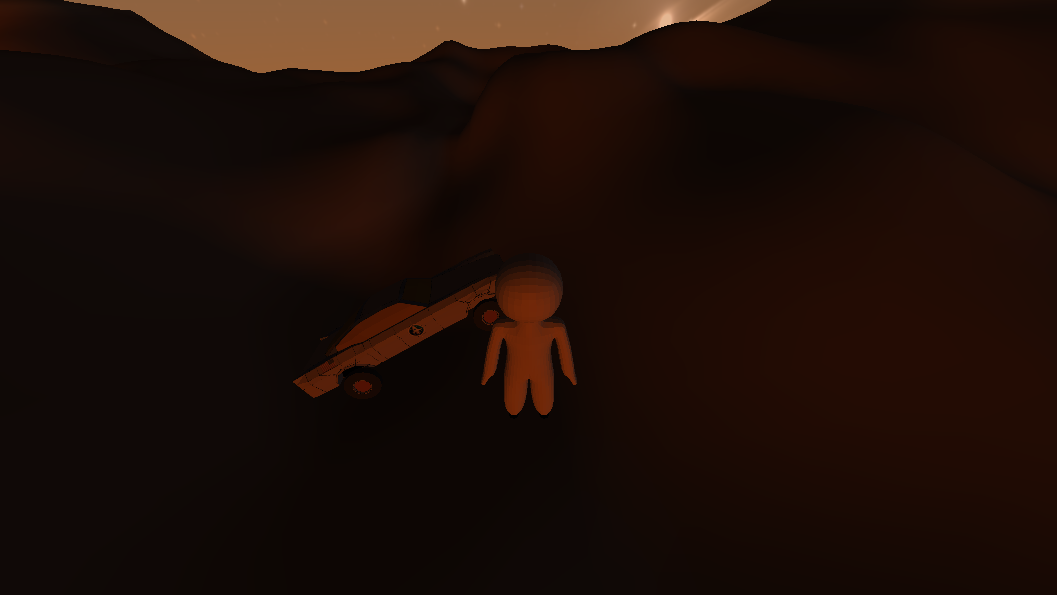
\includegraphics[width=0.8\textwidth]{chapters/lighting/sections/lighting/resources/directional-light.png}
    \caption{Directional light}
    \label{fig:directional-light}
\end{figure}
\subsection{Point lights}
In the game, spotlights are represented by white spherical lamps.

In Euclidean geometry, assuming that a point light is placed at a point $p$ and that the current fragment's position is given by $f$, we can calculate the light direction vector $l$ simply as
\begin{equation*}
    l = \frac{p - f}{d_E(p, f)},
\end{equation*}
where $d_E$ is the usual Euclidean distance, i.e.
\begin{equation} \label{eq:dist-euclidean}
    d_E(a, b) = \sqrt{\langle a - b, a - b\rangle_E}.
\end{equation}
For non-Euclidean geometries, we use modified formulas given by \cite{Szirmay-Kalos2022}, namely
\begin{equation}
    l = \frac{p - f \cos(d_S(p, f))}{\sin(d_S(p, f))}
\end{equation}
for spherical geometry and
\begin{equation}
    l = \frac{p - f\cosh(d_H(p, f))}{\sinh(d_H(p, f))}
\end{equation}
for hyperbolic geometry.
The spherical and hyperbolic distances $d_S$ and $d_H$ are given by
\begin{equation} \label{eq:dist-spherical}
    d_S(a, b) = \cos^{-1}(|\langle a, b \rangle_E|)
\end{equation}
and
\begin{equation} \label{eq:dist-hyperbolic}
    d_H(a, b) = \cosh^{-1}(-\langle a, b \rangle_L)
\end{equation}
respectively.

The important difference between a point light and a directional light is the \textit{attenuation} $a$.
Attenuation represents how the light's strength diminishes over distance.
It can be expressed as a reciprocal of a quadratic function:
\begin{equation}
    a = \frac{1}{K_c + K_l d + K_q d^2},
\end{equation}
where $d$ is the distance of the fragment from the source that can be calculated using one of the formulas \ref{eq:dist-euclidean}, \ref{eq:dist-spherical}, or \ref{eq:dist-hyperbolic} depending on the geometry.
Multiplying the light by the attenuation factor gives the desired effect of a realistic point light source such as a lamp, see \textcolor{red}{add figure}.
\subsection{Spotlights}
In the game, spotlights are used to represent the player's flashlight and the car's head- and tail lights.

Spotlights are modeled in the same way as point lights, with only one exception.
In the case of spotlights, we want to capture the fact that the light forms a cone.
To do that we calculate the \textit{intensity coefficient} given by
\begin{equation*}
    \mathrm{IC} = \frac{\langle l, -d \rangle - R}{r - R},
\end{equation*}
where $d$ is the vector along which the spotlight is directed, and $R$ and $r$ are the parameters defining the light cone \cite{LearnOpenGL-Light-casters}.
The intensity coefficient is then used to multiply each component of the light, giving the result shown in \textcolor{red}{add figure}.
\chapter{Results}
\todo{Add some introduction.}
The project that was created as the practical part of the thesis is the \textit{Hyper} video game available at \url{https://github.com/Non-Euclidean-World/Hyper}.

\section{Performance}
The performance and resource utilization of the game has been tested using Visual Studio's performance profiler\footnote{\url{https://learn.microsoft.com/en-us/visualstudio/profiling/?view=vs-2022}}.
The analysis was focused on three aspects:
\begin{enumerate}
    \item File I/O,
    \item CPU usage,
    \item memory usage.
\end{enumerate}
The data was collected on a machine running on x64-based Windows 11 with Intel(R) Core(TM) i7-9750H CPU, 32 GB of RAM, and NVIDIA GeForce GTX 1650 GPU.
During the first minute of the data collection, the player was running constantly, approximately in one direction, while modifying the terrain at the same time.
Starting at the 1-minute mark, the player turned around and started running in the opposite direction, still modifying the terrain, and also shooting at the bots from time to time.
The results of the profiling are shown in \autoref{fig:diag-session}.
\begin{figure}[h]
    \centering
    \includegraphics[width=1\textwidth]{chapters/results/sections/performance/resources/diag-session.png}
    \caption{Resource utilization of the game}
    \label{fig:diag-session}
\end{figure}

The "File Reads" graph shows the amount of data read in MB.
The initial spike in the file reads corresponds to the game reading the shader files and PNG files with textures.
It can be seen that starting at the 1-minute mark, there are frequent file reads.
This is because the chunks that were generated (and subsequently removed from the game and saved) during the initial run in one direction are now being revisited by the player and read from the disk.

The "Process Memory" graph shows that the memory usage remains approximately constant at around 350 MB.

The "CPU" graph shows that the CPU utilization peaks at around 10\%.

The total amount of disk space required to store the game saves for this session was 100 MB.
\section{Gameplay}
\textit{Hyper} was designed as an \textit{open world} game.
In a game of this type, the player is not constrained to achieving a specific goal and has a large degree of freedom to explore, interact with, or modify the game environment \cite{Open-World-MW}.
In this section, we'll show the various aspects of this concept in our game.

\subsection{Terrain editing}
The player has three "terrain modifiers", represented with pickaxe symbols, at their disposal.
Using the terrain modifier, the player can edit the game's landscape by building new structures or digging in the ground.
As an example of the "creation capabilities", we show in \autoref{fig:hyper-logo} how the letters making up the game's name could be created inside the game.
\begin{figure}[!htb]
    \centering
    \includegraphics[width=0.8\textwidth]{chapters/results/sections/gameplay/resources/hyper-logo-night-2.png}
    \caption{The letters of the word "Hyper" created in the game}
    \label{fig:hyper-logo}
\end{figure}

As mentioned before the terrain modifiers can also be used for carving in the terrain.
To illustrate that, in \autoref{fig:tunnel-under-hill} we show a tunnel that was dug through a hill.
\begin{figure}[!htb]
    \centering
    \includegraphics[width=0.8\textwidth]{chapters/results/sections/gameplay/resources/tunnel-with-car.png}
    \caption{Tunnel dug under a hill}
    \label{fig:tunnel-under-hill}
\end{figure}

\subsection{Exploring the game world}
The game starts in one of the various "landscapes" such as a desert, a forest, etc. each characterized by different terrain generation parameters and colors.

To make exploring the game world easier, the player can get into a car that moves considerably faster than the player.
\autoref{fig:car-in-hyperbolic} shows the car driving in hyperbolic space.
\begin{figure}[!htb]
    \centering
    \includegraphics[width=0.8\textwidth]{chapters/results/sections/gameplay/resources/car-in-hyperbolic.png}
    \caption{Riding a car in hyperbolic space}
    \label{fig:car-in-hyperbolic}
\end{figure}
Even though the car is much faster than the player it can roll over when traversing a particularly bumpy terrain.
For this reason, we included an option to flip the car back on its wheels when that happens.
\subsection{Interacting with the world's inhabitants}
To make the world more interactive we decided to populate it with NPCs also called bots.
Bots can be either hostile toward the player or neutral.
Hostile bots shoot projectiles and walk toward the player once they get into the player's proximity.
A group of bots shooting projectiles at the player in spherical space is shown in \autoref{fig:firing-squad}.
\begin{figure}[!htb]
    \centering
    \includegraphics[width=0.8\textwidth]{chapters/results/sections/gameplay/resources/firing-squad.png}
    \caption{Fighting with bots}
    \label{fig:firing-squad}
\end{figure}
The neutral bots are unbothered by the player's presence and just walk around.
This can change, however.
Once the player shoots at a neutral bot, it'll become hostile.
\subsection{Physics}\label{subsec:physics}
BepuPhysics2 proved to be an excellent choice for a video game physics engine.
Our tests, such as the one depicted in \autoref{fig:bepu-lots-of-stuff} show that it's able to handle large workloads.
In this particular test, we spawned 100 bots, each firing projectiles at the player.
Despite this workload on the physics engine, the application still managed to work without lags.
\begin{figure}[h]
    \centering
    \includegraphics[width=0.8\textwidth]{chapters/results/sections/gameplay/resources/lots-of-stuff.png}
    \caption{BepuPhysics library taken to the extremee}
    \label{fig:bepu-lots-of-stuff}
\end{figure}
\section{Depicting non-Euclidean spaces}
One of the main features of the game is the ability to explore non-Euclidean spaces.
To assess our depictions of non-Euclidean spaces, we decided to compare them with the ones from the game \textit{Hyperbolica}\footnote{\url{https://codeparade.itch.io/hyperbolica}} by \textit{CodeParade}.
It should be noted that the approach used in our game, although relatively simple makes it impossible to capture some of the interesting properties of non-Euclidean geometry, like tiling the plane with right-angled regular pentagons in hyperbolic space.

\subsection{Hyperbolic space}
From the visual standpoint, the hyperbolic space can be identified by the fact that the otherwise flat terrain appears "curved downward".
This may create an illusion that the terrain is wrapped around a giant sphere.
However, by exploring the hyperbolic space, we can quickly notice that it is infinite, just like the Euclidean space.
\autoref{fig:hyperbolic-space-games} shows the comparison of the depictions of hyperbolic space between our game and \textit{Hyperbolica}.
\begin{figure*}[h]
    \centering
    \begin{subfigure}[b]{0.475\textwidth}
        \centering
        \includegraphics[width=\textwidth]{chapters/results/sections/non_euclidean/resources/hyperbolic-in-hyper.png}
        \caption[]%
        {{\small \textit{Hyper}}}
        \label{fig:hyperbolic-space-games-hyper}
    \end{subfigure}
    \hfill
    \begin{subfigure}[b]{0.475\textwidth}
        \centering
        \includegraphics[width=\textwidth]{chapters/results/sections/non_euclidean/resources/hyperbolica-hyperbolic.png}
        \caption[]%
        {{\small \textit{Hyperbolica \cite{Hyperbolica-Hyperbolic}}}}
        \label{fig:hyperbolic-space-games-hyperbolica}
    \end{subfigure}
    \caption[]
    {\small Hyperbolic space}
    \label{fig:hyperbolic-space-games}
\end{figure*}

As mentioned in \autoref{subsubsec:practical-considerations-hyperbolic-space} in our approach the camera's position (as passed to the view matrix) is fixed.
Changing the point where it is located allows us to change the curvature of the terrain.
\autoref{fig:hyperbolic-space-curvatures} shows the scene in hyperbolic space where the camera is positioned close to the origin (cf. \autoref{fig:hyperbolic-space-small-curvature}) resulting in small curvature as compared to the scene when the camera is moved farther from the origin (cf. \autoref{fig:hyperbolic-space-big-curvature}).
\begin{figure*}[h]
    \centering
    \begin{subfigure}[b]{0.475\textwidth}
        \centering
        \includegraphics[width=\textwidth]{chapters/results/sections/non_euclidean/resources/hyperbolic-small-curvature.png}
        \caption[]%
        {{\small Camera close to the origin}}
        \label{fig:hyperbolic-space-small-curvature}
    \end{subfigure}
    \hfill
    \begin{subfigure}[b]{0.475\textwidth}
        \centering
        \includegraphics[width=\textwidth]{chapters/results/sections/non_euclidean/resources/hyperbolic-large-curvature.png}
        \caption[]%
        {{\small Camera far from the origin}}
        \label{fig:hyperbolic-space-big-curvature}
    \end{subfigure}
    \caption[]
    {\small Hyperbolic space, different curvatures due to camera's position}
    \label{fig:hyperbolic-space-curvatures}
\end{figure*}

\question{Do we have to mention that our non-Euclidean spaces are "fake" in the sense that you don't have 5-sided right pentagons.}
\subsection{Spherical space}
Playing the video game in spherical space gives the impression that the terrain is wallpapered onto the inside of a giant sphere.
Unlike the hyperbolic space, the spherical space is finite.
Comparison in \autoref{fig:spherical-space-games} shows that our implementation provides visual effects to a certain degree similar to those in \textit{Hyperbolica}.
\begin{figure*}[h]
    \centering
    \begin{subfigure}[b]{0.475\textwidth}
        \centering
        \includegraphics[width=\textwidth]{chapters/results/sections/non_euclidean/resources/spherical-in-hyper.png}
        \caption[]%
        {{\small \textit{Hyper}}}
        \label{fig:spherical-space-games-hyper}
    \end{subfigure}
    \hfill
    \begin{subfigure}[b]{0.5\textwidth}
        \centering
        \includegraphics[width=\textwidth]{chapters/results/sections/non_euclidean/resources/hyperbolica-1.png}
        \caption[]%
        {{\small \textit{Hyperbolica \cite{Hyperbolica-Spherical}}}}
        \label{fig:spherical-space-games-hyperbolica}
    \end{subfigure}
    \caption[]
    {\small Spherical space}
    \label{fig:spherical-space-games}
\end{figure*}

\todo{Add chapter with results (what we accomplished, what we failed to accomplish, plans for future development, etc.)}

% ------------------------------- BIBLIOGRAPHY ---------------------------
% LEXICOGRAPHICAL ORDER BY AUTHORS' LAST NAMES
% FOR AMBITIOUS ONES - USE BIBTEX


\printbibliography
\pagenumbering{gobble}
\thispagestyle{empty}



% ----------------------- LIST OF SYMBOLS AND ABBREVIATIONS ------------------
\chapter*{List of symbols and abbreviations}

\begin{tabular}{cl}
  nzw.           & nadzwyczajny  \\
  *              & star operator \\
  $\widetilde{}$ & tilde
\end{tabular}
\\
If you don't need it, delete it.
\thispagestyle{empty}


% ----------------------------  LIST OF FIGURES --------------------------------
\listoffigures
\thispagestyle{empty}
If you don't need it, delete it.


% -----------------------------  LIST OF TABLES --------------------------------
\listoftables
\thispagestyle{empty}
If you don't need it, delete it.

% -----------------------------  LIST OF APPENDICES ---------------------------
\chapter*{List of appendices}
\begin{enumerate}
  \item Appendix 1
  \item Appendix 2
  \item In case of no appendices, delete this part.
\end{enumerate}
\thispagestyle{empty}


\end{document}
